\subsection{Global parameters}
\label{parameters:global}


\begin{itemize}
\item {\it Parameter name:} {\tt Additional shared libraries}
\phantomsection\label{parameters:Additional shared libraries}


\index[prmindex]{Additional shared libraries}
\index[prmindexfull]{Additional shared libraries}
{\it Value:} 


{\it Default:} 


{\it Description:} A list of names of additional shared libraries that should be loaded upon starting up the program. The names of these files can contain absolute or relative paths (relative to the directory in which you call ASPECT). In fact, file names that are do not contain any directory information (i.e., only the name of a file such as <myplugin.so> will not be found if they are not located in one of the directories listed in the \texttt{LD_LIBRARY_PATH} environment variable. In order to load a library in the current directory, use <./myplugin.so> instead.

The typical use of this parameter is so that you can implement additional plugins in your own directories, rather than in the ASPECT source directories. You can then simply compile these plugins into a shared library without having to re-compile all of ASPECT. See the section of the manual discussing writing extensions for more information on how to compile additional files into a shared library.


{\it Possible values:} [List list of <[FileName (Type: input)]> of length 0...4294967295 (inclusive)]
\item {\it Parameter name:} {\tt Adiabatic surface temperature}
\phantomsection\label{parameters:Adiabatic surface temperature}


\index[prmindex]{Adiabatic surface temperature}
\index[prmindexfull]{Adiabatic surface temperature}
{\it Value:} 0


{\it Default:} 0


{\it Description:} In order to make the problem in the first time step easier to solve, we need a reasonable guess for the temperature and pressure. To obtain it, we use an adiabatic pressure and temperature field. This parameter describes what the `adiabatic' temperature would be at the surface of the domain (i.e. at depth zero). Note that this value need not coincide with the boundary condition posed at this point. Rather, the boundary condition may differ significantly from the adiabatic value, and then typically induce a thermal boundary layer.

For more information, see the section in the manual that discusses the general mathematical model.


{\it Possible values:} [Double -1.79769e+308...1.79769e+308 (inclusive)]
\item {\it Parameter name:} {\tt CFL number}
\phantomsection\label{parameters:CFL number}


\index[prmindex]{CFL number}
\index[prmindexfull]{CFL number}
{\it Value:} 1.0


{\it Default:} 1.0


{\it Description:} In computations, the time step $k$ is chosen according to $k = c \min_K \frac {h_K} {\|u\|_{\infty,K} p_T}$ where $h_K$ is the diameter of cell $K$, and the denominator is the maximal magnitude of the velocity on cell $K$ times the polynomial degree $p_T$ of the temperature discretization. The dimensionless constant $c$ is called the CFL number in this program. For time discretizations that have explicit components, $c$ must be less than a constant that depends on the details of the time discretization and that is no larger than one. On the other hand, for implicit discretizations such as the one chosen here, one can choose the time step as large as one wants (in particular, one can choose $c>1$) though a CFL number significantly larger than one will yield rather diffusive solutions. Units: None.


{\it Possible values:} [Double 0...1.79769e+308 (inclusive)]
\item {\it Parameter name:} {\tt Composition solver tolerance}
\phantomsection\label{parameters:Composition solver tolerance}


\index[prmindex]{Composition solver tolerance}
\index[prmindexfull]{Composition solver tolerance}
{\it Value:} 1e-12


{\it Default:} 1e-12


{\it Description:} The relative tolerance up to which the linear system for the composition system gets solved. See 'linear solver tolerance' for more details.


{\it Possible values:} [Double 0...1 (inclusive)]
\item {\it Parameter name:} {\tt Dimension}
\phantomsection\label{parameters:Dimension}


\index[prmindex]{Dimension}
\index[prmindexfull]{Dimension}
{\it Value:} 3


{\it Default:} 2


{\it Description:} The number of space dimensions you want to run this program in. ASPECT can run in 2 and 3 space dimensions.


{\it Possible values:} [Integer range 2...4 (inclusive)]
\item {\it Parameter name:} {\tt End time}
\phantomsection\label{parameters:End time}


\index[prmindex]{End time}
\index[prmindexfull]{End time}
{\it Value:} 0


{\it Default:} 5.69e+300


{\it Description:} The end time of the simulation. The default value is a number so that when converted from years to seconds it is approximately equal to the largest number representable in floating point arithmetic. For all practical purposes, this equals infinity. Units: Years if the 'Use years in output instead of seconds' parameter is set; seconds otherwise.


{\it Possible values:} [Double -1.79769e+308...1.79769e+308 (inclusive)]
\item {\it Parameter name:} {\tt Linear solver tolerance}
\phantomsection\label{parameters:Linear solver tolerance}


\index[prmindex]{Linear solver tolerance}
\index[prmindexfull]{Linear solver tolerance}
{\it Value:} 1e-4


{\it Default:} 1e-7


{\it Description:} A relative tolerance up to which the linear Stokes systems in each time or nonlinear step should be solved. The absolute tolerance will then be $\| M x_0 - F \| \cdot \text{tol}$, where $x_0 = (0,p_0)$ is the initial guess of the pressure, $M$ is the system matrix, F is the right-hand side, and tol is the parameter specified here. We include the initial guess of the pressure to remove the dependency of the tolerance on the static pressure. A given tolerance value of 1 would mean that a zero solution vector is an acceptable solution since in that case the norm of the residual of the linear system equals the norm of the right hand side. A given tolerance of 0 would mean that the linear system has to be solved exactly, since this is the only way to obtain a zero residual.

In practice, you should choose the value of this parameter to be so that if you make it smaller the results of your simulation do not change any more (qualitatively) whereas if you make it larger, they do. For most cases, the default value should be sufficient. In fact, a tolerance of 1e-4 might be accurate enough.


{\it Possible values:} [Double 0...1 (inclusive)]
\item {\it Parameter name:} {\tt Max nonlinear iterations}
\phantomsection\label{parameters:Max nonlinear iterations}


\index[prmindex]{Max nonlinear iterations}
\index[prmindexfull]{Max nonlinear iterations}
{\it Value:} 6


{\it Default:} 10


{\it Description:} The maximal number of nonlinear iterations to be performed.


{\it Possible values:} [Integer range 0...2147483647 (inclusive)]
\item {\it Parameter name:} {\tt Maximum time step}
\phantomsection\label{parameters:Maximum time step}


\index[prmindex]{Maximum time step}
\index[prmindexfull]{Maximum time step}
{\it Value:} 5.69e+300


{\it Default:} 5.69e+300


{\it Description:} Set a maximum time step size for the solver to use. Generally the time step based on the CFL number should be sufficient, but for complicated models or benchmarking it may be useful to limit the time step to some value. The default value is a value so that when converted from years into seconds it equals the largest number representable by a floating point number, implying an unlimited time step.Units: Years or seconds, depending on the ``Use years in output instead of seconds'' parameter.


{\it Possible values:} [Double 0...1.79769e+308 (inclusive)]
\item {\it Parameter name:} {\tt Nonlinear solver scheme}
\phantomsection\label{parameters:Nonlinear solver scheme}


\index[prmindex]{Nonlinear solver scheme}
\index[prmindexfull]{Nonlinear solver scheme}
{\it Value:} iterated Stokes


{\it Default:} IMPES


{\it Description:} The kind of scheme used to resolve the nonlinearity in the system. 'IMPES' is the classical IMplicit Pressure Explicit Saturation scheme in which ones solves the temperatures and Stokes equations exactly once per time step, one after the other. The 'iterated IMPES' scheme iterates this decoupled approach by alternating the solution of the temperature and Stokes systems. The 'iterated Stokes' scheme solves the temperature equation once at the beginning of each time step and then iterates out the solution of the Stokes equation. The 'Stokes only' scheme only solves the Stokes system and ignores compositions and the temperature equation (careful, the material model must not depend on the temperature; mostly useful for Stokes benchmarks). The 'Advection only'scheme only solves the temperature and other advection systems and instead of solving for the Stokes system, a prescribed velocity and pressure is used


{\it Possible values:} [Selection IMPES|iterated IMPES|iterated Stokes|Stokes only|Advection only ]
\item {\it Parameter name:} {\tt Nonlinear solver tolerance}
\phantomsection\label{parameters:Nonlinear solver tolerance}


\index[prmindex]{Nonlinear solver tolerance}
\index[prmindexfull]{Nonlinear solver tolerance}
{\it Value:} 1e-4


{\it Default:} 1e-5


{\it Description:} A relative tolerance up to which the nonlinear solver will iterate. This parameter is only relevant if Nonlinear solver scheme is set to 'iterated Stokes' or 'iterated IMPES'.


{\it Possible values:} [Double 0...1 (inclusive)]
\item {\it Parameter name:} {\tt Number of cheap Stokes solver steps}
\phantomsection\label{parameters:Number of cheap Stokes solver steps}


\index[prmindex]{Number of cheap Stokes solver steps}
\index[prmindexfull]{Number of cheap Stokes solver steps}
{\it Value:} 0


{\it Default:} 30


{\it Description:} As explained in the ASPECT paper (Kronbichler, Heister, and Bangerth, GJI 2012) we first try to solve the Stokes system in every time step using a GMRES iteration with a poor but cheap preconditioner. By default, we try whether we can converge the GMRES solver in 30 such iterations before deciding that we need a better preconditioner. This is sufficient for simple problems with constant viscosity and we never need the second phase with the more expensive preconditioner. On the other hand, for more complex problems, and in particular for problems with strongly varying viscosity, the 30 cheap iterations don't actually do very much good and one might skip this part right away. In that case, this parameter can be set to zero, i.e., we immediately start with the better but more expensive preconditioner.


{\it Possible values:} [Integer range 0...2147483647 (inclusive)]
\item {\it Parameter name:} {\tt Output directory}
\phantomsection\label{parameters:Output directory}


\index[prmindex]{Output directory}
\index[prmindexfull]{Output directory}
{\it Value:} africa_litho1.0_crust1.0_g3_harmAvg


{\it Default:} output


{\it Description:} The name of the directory into which all output files should be placed. This may be an absolute or a relative path.


{\it Possible values:} [DirectoryName]
\item {\it Parameter name:} {\tt Pressure normalization}
\phantomsection\label{parameters:Pressure normalization}


\index[prmindex]{Pressure normalization}
\index[prmindexfull]{Pressure normalization}
{\it Value:} surface


{\it Default:} surface


{\it Description:} If and how to normalize the pressure after the solution step. This is necessary because depending on boundary conditions, in many cases the pressure is only determined by the model up to a constant. On the other hand, we often would like to have a well-determined pressure, for example for table lookups of material properties in models or for comparing solutions. If the given value is `surface', then normalization at the end of each time steps adds a constant value to the pressure in such a way that the average pressure at the surface of the domain is zero; the surface of the domain is determined by asking the geometry model whether a particular face of the geometry has a zero or small `depth'. If the value of this parameter is `volume' then the pressure is normalized so that the domain average is zero. If `no' is given, the no pressure normalization is performed.


{\it Possible values:} [Selection surface|volume|no ]
\item {\it Parameter name:} {\tt Resume computation}
\phantomsection\label{parameters:Resume computation}


\index[prmindex]{Resume computation}
\index[prmindexfull]{Resume computation}
{\it Value:} false


{\it Default:} false


{\it Description:} A flag indicating whether the computation should be resumed from a previously saved state (if true) or start from scratch (if false).


{\it Possible values:} [Bool]
\item {\it Parameter name:} {\tt Start time}
\phantomsection\label{parameters:Start time}


\index[prmindex]{Start time}
\index[prmindexfull]{Start time}
{\it Value:} 0


{\it Default:} 0


{\it Description:} The start time of the simulation. Units: Years if the 'Use years in output instead of seconds' parameter is set; seconds otherwise.


{\it Possible values:} [Double -1.79769e+308...1.79769e+308 (inclusive)]
\item {\it Parameter name:} {\tt Surface pressure}
\phantomsection\label{parameters:Surface pressure}


\index[prmindex]{Surface pressure}
\index[prmindexfull]{Surface pressure}
{\it Value:} 0


{\it Default:} 0


{\it Description:} The mathematical equations that describe thermal convection only determine the pressure up to an arbitrary constant. On the other hand, for comparison and for looking up material parameters it is important that the pressure be normalized somehow. We do this by enforcing a particular average pressure value at the surface of the domain, where the geometry model determines where the surface is. This parameter describes what this average surface pressure value is supposed to be. By default, it is set to zero, but one may want to choose a different value for example for simulating only the volume of the mantle below the lithosphere, in which case the surface pressure should be the lithostatic pressure at the bottom of the lithosphere.

For more information, see the section in the manual that discusses the general mathematical model.


{\it Possible values:} [Double -1.79769e+308...1.79769e+308 (inclusive)]
\item {\it Parameter name:} {\tt Temperature solver tolerance}
\phantomsection\label{parameters:Temperature solver tolerance}


\index[prmindex]{Temperature solver tolerance}
\index[prmindexfull]{Temperature solver tolerance}
{\it Value:} 1e-4


{\it Default:} 1e-12


{\it Description:} The relative tolerance up to which the linear system for the temperature system gets solved. See 'linear solver tolerance' for more details.


{\it Possible values:} [Double 0...1 (inclusive)]
\item {\it Parameter name:} {\tt Timing output frequency}
\phantomsection\label{parameters:Timing output frequency}


\index[prmindex]{Timing output frequency}
\index[prmindexfull]{Timing output frequency}
{\it Value:} 100


{\it Default:} 100


{\it Description:} How frequently in timesteps to output timing information. This is generally adjusted only for debugging and timing purposes. If the value is set to zero it will also output timing information at the initiation timesteps.


{\it Possible values:} [Integer range 0...2147483647 (inclusive)]
\item {\it Parameter name:} {\tt Use conduction timestep}
\phantomsection\label{parameters:Use conduction timestep}


\index[prmindex]{Use conduction timestep}
\index[prmindexfull]{Use conduction timestep}
{\it Value:} false


{\it Default:} false


{\it Description:} Mantle convection simulations are often focused on convection dominated systems. However, these codes can also be used to investigate systems where heat conduction plays a dominant role. This parameter indicates whether the simulator should also use heat conduction in determining the length of each time step.


{\it Possible values:} [Bool]
\item {\it Parameter name:} {\tt Use direct solver for Stokes system}
\phantomsection\label{parameters:Use direct solver for Stokes system}


\index[prmindex]{Use direct solver for Stokes system}
\index[prmindexfull]{Use direct solver for Stokes system}
{\it Value:} false


{\it Default:} false


{\it Description:} If set to true the linear system for the Stokes equation will be solved using Trilinos klu, otherwise an iterative Schur complement solver is used. The direct solver is only efficient for small problems.


{\it Possible values:} [Bool]
\item {\it Parameter name:} {\tt Use years in output instead of seconds}
\phantomsection\label{parameters:Use years in output instead of seconds}


\index[prmindex]{Use years in output instead of seconds}
\index[prmindexfull]{Use years in output instead of seconds}
{\it Value:} true


{\it Default:} true


{\it Description:} When computing results for mantle convection simulations, it is often difficult to judge the order of magnitude of results when they are stated in MKS units involving seconds. Rather, some kinds of results such as velocities are often stated in terms of meters per year (or, sometimes, centimeters per year). On the other hand, for non-dimensional computations, one wants results in their natural unit system as used inside the code. If this flag is set to 'true' conversion to years happens; if it is 'false', no such conversion happens. Note that when 'true', some input such as prescribed velocities should also use years instead of seconds.


{\it Possible values:} [Bool]
\end{itemize}



\subsection{Parameters in section \tt Adiabatic conditions model}
\label{parameters:Adiabatic_20conditions_20model}

\begin{itemize}
\item {\it Parameter name:} {\tt Model name}
\phantomsection\label{parameters:Adiabatic conditions model/Model name}


\index[prmindex]{Model name}
\index[prmindexfull]{Adiabatic conditions model!Model name}
{\it Value:} initial profile


{\it Default:} initial profile


{\it Description:} Select one of the following models:

`initial profile': A model in which the adiabatic profile is calculated once at the start of the model run. The gravity is assumed to be in depth direction and the composition is evaluated at reference points, no lateral averaging is performed. All material parameters are used from the material model plugin.


{\it Possible values:} [Selection initial profile ]
\end{itemize}

\subsection{Parameters in section \tt Boundary composition model}
\label{parameters:Boundary_20composition_20model}

\begin{itemize}
\item {\it Parameter name:} {\tt Model name}
\phantomsection\label{parameters:Boundary composition model/Model name}


\index[prmindex]{Model name}
\index[prmindexfull]{Boundary composition model!Model name}
{\it Value:} 


{\it Default:} 


{\it Description:} Select one of the following models:

`ascii data': Implementation of a model in which the boundary composition is derived from files containing data in ascii format. Note the required format of the input data: The first lines may contain any number of commentsif they begin with '#', but one of these lines needs tocontain the number of grid points in each dimension asfor example '# POINTS: 3 3'.The order of the data columns has to be 'x', 'composition1', 'composition2', etc. in a 2d model and 'x', 'y', 'composition1', 'composition2', etc., in a 3d model, according to the number of compositional fields, which means that there has to be a single column for every composition in the model.Note that the data in the input files need to be sorted in a specific order: the first coordinate needs to ascend first, followed by the second in order to assign the correct data to the prescribed coordinates.If you use a spherical model, then the data will still be handled as cartesian,however the assumed grid changes. 'x' will be replaced by the radial distance of the point to the bottom of the model, 'y' by the azimuth angle and 'z' by the polar angle measured positive from the north pole. The grid will be assumed to be a latitude-longitude grid. Note that the order of spherical coordinates is 'r', 'phi', 'theta' and not 'r', 'theta', 'phi', since this allows for dimension independent expressions. 

`box': A model in which the composition is chosen constant on all the sides of a box.

`initial composition': A model in which the composition at the boundary is chosen to be the same as given in the initial conditions.

Because this class simply takes what the initial composition had described, this class can not know certain pieces of information such as the minimal and maximal composition on the boundary. For operations that require this, for example in postprocessing, this boundary composition model must therefore be told what the minimal and maximal values on the boundary are. This is done using parameters set in section ``Boundary composition model/Initial composition''.

`spherical constant': A model in which the composition is chosen constant on the inner and outer boundaries of a spherical shell. Parameters are read from subsection 'Spherical constant'.


{\it Possible values:} [Selection ascii data|box|initial composition|spherical constant ]
\end{itemize}



\subsection{Parameters in section \tt Boundary composition model/Ascii data model}
\label{parameters:Boundary_20composition_20model/Ascii_20data_20model}

\begin{itemize}
\item {\it Parameter name:} {\tt Data directory}
\phantomsection\label{parameters:Boundary composition model/Ascii data model/Data directory}


\index[prmindex]{Data directory}
\index[prmindexfull]{Boundary composition model!Ascii data model!Data directory}
{\it Value:} $ASPECT_SOURCE_DIR/data/boundary-composition/ascii-data/test/


{\it Default:} $ASPECT_SOURCE_DIR/data/boundary-composition/ascii-data/test/


{\it Description:} The name of a directory that contains the model data. This path may either be absolute (if starting with a '/') or relative to the current directory. The path may also include the special text '$ASPECT_SOURCE_DIR' which will be interpreted as the path in which the ASPECT source files were located when ASPECT was compiled. This interpretation allows, for example, to reference files located in the 'data/' subdirectory of ASPECT. 


{\it Possible values:} [DirectoryName]
\item {\it Parameter name:} {\tt Data file name}
\phantomsection\label{parameters:Boundary composition model/Ascii data model/Data file name}


\index[prmindex]{Data file name}
\index[prmindexfull]{Boundary composition model!Ascii data model!Data file name}
{\it Value:} box_2d_%s.%d.txt


{\it Default:} box_2d_%s.%d.txt


{\it Description:} The file name of the material data. Provide file in format: (Velocity file name).\%s\%d where \%s is a string specifying the boundary of the model according to the names of the boundary indicators (of a box or a spherical shell).\%d is any sprintf integer qualifier, specifying the format of the current file number. 


{\it Possible values:} [Anything]
\item {\it Parameter name:} {\tt Data file time step}
\phantomsection\label{parameters:Boundary composition model/Ascii data model/Data file time step}


\index[prmindex]{Data file time step}
\index[prmindexfull]{Boundary composition model!Ascii data model!Data file time step}
{\it Value:} 1e6


{\it Default:} 1e6


{\it Description:} Time step between following velocity files. Depending on the setting of the global 'Use years in output instead of seconds' flag in the input file, this number is either interpreted as seconds or as years. The default is one million, i.e., either one million seconds or one million years.


{\it Possible values:} [Double 0...1.79769e+308 (inclusive)]
\item {\it Parameter name:} {\tt Decreasing file order}
\phantomsection\label{parameters:Boundary composition model/Ascii data model/Decreasing file order}


\index[prmindex]{Decreasing file order}
\index[prmindexfull]{Boundary composition model!Ascii data model!Decreasing file order}
{\it Value:} false


{\it Default:} false


{\it Description:} In some cases the boundary files are not numbered in increasing but in decreasing order (e.g. 'Ma BP'). If this flag is set to 'True' the plugin will first load the file with the number 'First velocity file number' and decrease the file number during the model run.


{\it Possible values:} [Bool]
\item {\it Parameter name:} {\tt First data file model time}
\phantomsection\label{parameters:Boundary composition model/Ascii data model/First data file model time}


\index[prmindex]{First data file model time}
\index[prmindexfull]{Boundary composition model!Ascii data model!First data file model time}
{\it Value:} 0


{\it Default:} 0


{\it Description:} Time from which on the velocity file with number 'First velocity file number' is used as boundary condition. Previous to this time, a no-slip boundary condition is assumed. Depending on the setting of the global 'Use years in output instead of seconds' flag in the input file, this number is either interpreted as seconds or as years.


{\it Possible values:} [Double 0...1.79769e+308 (inclusive)]
\item {\it Parameter name:} {\tt First data file number}
\phantomsection\label{parameters:Boundary composition model/Ascii data model/First data file number}


\index[prmindex]{First data file number}
\index[prmindexfull]{Boundary composition model!Ascii data model!First data file number}
{\it Value:} 0


{\it Default:} 0


{\it Description:} Number of the first velocity file to be loaded when the model time is larger than 'First velocity file model time'.


{\it Possible values:} [Integer range -2147483648...2147483647 (inclusive)]
\item {\it Parameter name:} {\tt Scale factor}
\phantomsection\label{parameters:Boundary composition model/Ascii data model/Scale factor}


\index[prmindex]{Scale factor}
\index[prmindexfull]{Boundary composition model!Ascii data model!Scale factor}
{\it Value:} 1


{\it Default:} 1


{\it Description:} Scalar factor, which is applied to the boundary velocity. You might want to use this to scale the velocities to a reference model (e.g. with free-slip boundary) or another plate reconstruction. Another way to use this factor is to convert units of the input files. The unit is assumed to bem/s or m/yr depending on the 'Use years in output instead of seconds' flag. If you provide velocities in cm/yr set this factor to 0.01.


{\it Possible values:} [Double 0...1.79769e+308 (inclusive)]
\end{itemize}

\subsection{Parameters in section \tt Boundary composition model/Box}
\label{parameters:Boundary_20composition_20model/Box}

\begin{itemize}
\item {\it Parameter name:} {\tt Back composition}
\phantomsection\label{parameters:Boundary composition model/Box/Back composition}


\index[prmindex]{Back composition}
\index[prmindexfull]{Boundary composition model!Box!Back composition}
{\it Value:} 


{\it Default:} 


{\it Description:} A comma separated list of composition boundary values at the back boundary (at maximal y-value). This list must have as many entries as there are compositional fields. Units: none.


{\it Possible values:} [List list of <[Double -1.79769e+308...1.79769e+308 (inclusive)]> of length 0...4294967295 (inclusive)]
\item {\it Parameter name:} {\tt Bottom composition}
\phantomsection\label{parameters:Boundary composition model/Box/Bottom composition}


\index[prmindex]{Bottom composition}
\index[prmindexfull]{Boundary composition model!Box!Bottom composition}
{\it Value:} 


{\it Default:} 


{\it Description:} A comma separated list of composition boundary values at the bottom boundary (at minimal y-value in 2d, or minimal z-value in 3d). This list must have as many entries as there are compositional fields. Units: none.


{\it Possible values:} [List list of <[Double -1.79769e+308...1.79769e+308 (inclusive)]> of length 0...4294967295 (inclusive)]
\item {\it Parameter name:} {\tt Front composition}
\phantomsection\label{parameters:Boundary composition model/Box/Front composition}


\index[prmindex]{Front composition}
\index[prmindexfull]{Boundary composition model!Box!Front composition}
{\it Value:} 


{\it Default:} 


{\it Description:} A comma separated list of composition boundary values at the front boundary (at momimal y-value). This list must have as many entries as there are compositional fields. Units: none.


{\it Possible values:} [List list of <[Double -1.79769e+308...1.79769e+308 (inclusive)]> of length 0...4294967295 (inclusive)]
\item {\it Parameter name:} {\tt Left composition}
\phantomsection\label{parameters:Boundary composition model/Box/Left composition}


\index[prmindex]{Left composition}
\index[prmindexfull]{Boundary composition model!Box!Left composition}
{\it Value:} 


{\it Default:} 


{\it Description:} A comma separated list of composition boundary values at the left boundary (at minimal x-value). This list must have as many entries as there are compositional fields. Units: none.


{\it Possible values:} [List list of <[Double -1.79769e+308...1.79769e+308 (inclusive)]> of length 0...4294967295 (inclusive)]
\item {\it Parameter name:} {\tt Right composition}
\phantomsection\label{parameters:Boundary composition model/Box/Right composition}


\index[prmindex]{Right composition}
\index[prmindexfull]{Boundary composition model!Box!Right composition}
{\it Value:} 


{\it Default:} 


{\it Description:} A comma separated list of composition boundary values at the right boundary (at maximal x-value). This list must have as many entries as there are compositional fields. Units: none.


{\it Possible values:} [List list of <[Double -1.79769e+308...1.79769e+308 (inclusive)]> of length 0...4294967295 (inclusive)]
\item {\it Parameter name:} {\tt Top composition}
\phantomsection\label{parameters:Boundary composition model/Box/Top composition}


\index[prmindex]{Top composition}
\index[prmindexfull]{Boundary composition model!Box!Top composition}
{\it Value:} 


{\it Default:} 


{\it Description:} A comma separated list of composition boundary values at the top boundary (at maximal y-value in 2d, or maximal z-value in 3d). This list must have as many entries as there are compositional fields. Units: none.


{\it Possible values:} [List list of <[Double -1.79769e+308...1.79769e+308 (inclusive)]> of length 0...4294967295 (inclusive)]
\end{itemize}

\subsection{Parameters in section \tt Boundary composition model/Initial composition}
\label{parameters:Boundary_20composition_20model/Initial_20composition}

\begin{itemize}
\item {\it Parameter name:} {\tt Maximal composition}
\phantomsection\label{parameters:Boundary composition model/Initial composition/Maximal composition}


\index[prmindex]{Maximal composition}
\index[prmindexfull]{Boundary composition model!Initial composition!Maximal composition}
{\it Value:} 1


{\it Default:} 1


{\it Description:} Maximal composition. Units: none.


{\it Possible values:} [Double -1.79769e+308...1.79769e+308 (inclusive)]
\item {\it Parameter name:} {\tt Minimal composition}
\phantomsection\label{parameters:Boundary composition model/Initial composition/Minimal composition}


\index[prmindex]{Minimal composition}
\index[prmindexfull]{Boundary composition model!Initial composition!Minimal composition}
{\it Value:} 0


{\it Default:} 0


{\it Description:} Minimal composition. Units: none.


{\it Possible values:} [Double -1.79769e+308...1.79769e+308 (inclusive)]
\end{itemize}

\subsection{Parameters in section \tt Boundary composition model/Spherical constant}
\label{parameters:Boundary_20composition_20model/Spherical_20constant}

\begin{itemize}
\item {\it Parameter name:} {\tt Inner composition}
\phantomsection\label{parameters:Boundary composition model/Spherical constant/Inner composition}


\index[prmindex]{Inner composition}
\index[prmindexfull]{Boundary composition model!Spherical constant!Inner composition}
{\it Value:} 1


{\it Default:} 1


{\it Description:} Composition at the inner boundary (core mantle boundary). Units: none.


{\it Possible values:} [Double -1.79769e+308...1.79769e+308 (inclusive)]
\item {\it Parameter name:} {\tt Outer composition}
\phantomsection\label{parameters:Boundary composition model/Spherical constant/Outer composition}


\index[prmindex]{Outer composition}
\index[prmindexfull]{Boundary composition model!Spherical constant!Outer composition}
{\it Value:} 0


{\it Default:} 0


{\it Description:} Composition at the outer boundary (lithosphere water/air). Units: none.


{\it Possible values:} [Double -1.79769e+308...1.79769e+308 (inclusive)]
\end{itemize}

\subsection{Parameters in section \tt Boundary temperature model}
\label{parameters:Boundary_20temperature_20model}

\begin{itemize}
\item {\it Parameter name:} {\tt Model name}
\phantomsection\label{parameters:Boundary temperature model/Model name}


\index[prmindex]{Model name}
\index[prmindexfull]{Boundary temperature model!Model name}
{\it Value:} box


{\it Default:} 


{\it Description:} Select one of the following models:

`ascii data': Implementation of a model in which the boundary data is derived from files containing data in ascii format. Note the required format of the input data: The first lines may contain any number of commentsif they begin with '#', but one of these lines needs tocontain the number of grid points in each dimension asfor example '# POINTS: 3 3'.The order of the data columns has to be 'x', 'Temperature [K]' in a 2d model and  'x', 'y', 'Temperature [K]' in a 3d model, which means that there has to be a single column containing the temperature. Note that the data in the input files need to be sorted in a specific order: the first coordinate needs to ascend first, followed by the second in order to assign the correct data to the prescribed coordinates.If you use a spherical model, then the data will still be handled as cartesian,however the assumed grid changes. 'x' will be replaced by the radial distance of the point to the bottom of the model, 'y' by the azimuth angle and 'z' by the polar angle measured positive from the north pole. The grid will be assumed to be a latitude-longitude grid. Note that the order of spherical coordinates is 'r', 'phi', 'theta' and not 'r', 'theta', 'phi', since this allows for dimension independent expressions. 

`box': A model in which the temperature is chosen constant on all the sides of a box.

`constant': A model in which the temperature is chosen constant on a given boundary indicator.  Parameters are read from the subsection 'Constant'.

`function': Implementation of a model in which the boundary temperature is given in terms of an explicit formula that is elaborated in the parameters in section ``Boundary temperature model|Function''. 

Since the symbol $t$ indicating time may appear in the formulas for the prescribed temperatures, it is interpreted as having units seconds unless the global input parameter ``Use years in output instead of seconds'' is set, in which case we interpret the formula expressions as having units year.

Because this class simply takes what the function calculates, this class can not know certain pieces of information such as the minimal and maximal temperature on the boundary. For operations that require this, for example in postprocessing, this boundary temperature model must therefore be told what the minimal and maximal values on the boundary are. This is done using parameters set in section ``Boundary temperature model/Initial temperature''.

The format of these functions follows the syntax understood by the muparser library, see Section~\ref{sec:muparser-format}.

`initial temperature': A model in which the temperature at the boundary is chosen to be the same as given in the initial conditions.

Because this class simply takes what the initial temperature had described, this class can not know certain pieces of information such as the minimal and maximal temperature on the boundary. For operations that require this, for example in postprocessing, this boundary temperature model must therefore be told what the minimal and maximal values on the boundary are. This is done using parameters set in section ``Boundary temperature model/Initial temperature''.

`spherical constant': A model in which the temperature is chosen constant on the inner and outer boundaries of a spherical shell. Parameters are read from subsection 'Spherical constant'.


{\it Possible values:} [Selection ascii data|box|constant|function|initial temperature|spherical constant ]
\end{itemize}



\subsection{Parameters in section \tt Boundary temperature model/Ascii data model}
\label{parameters:Boundary_20temperature_20model/Ascii_20data_20model}

\begin{itemize}
\item {\it Parameter name:} {\tt Data directory}
\phantomsection\label{parameters:Boundary temperature model/Ascii data model/Data directory}


\index[prmindex]{Data directory}
\index[prmindexfull]{Boundary temperature model!Ascii data model!Data directory}
{\it Value:} $ASPECT_SOURCE_DIR/data/boundary-temperature/ascii-data/test/


{\it Default:} $ASPECT_SOURCE_DIR/data/boundary-temperature/ascii-data/test/


{\it Description:} The name of a directory that contains the model data. This path may either be absolute (if starting with a '/') or relative to the current directory. The path may also include the special text '$ASPECT_SOURCE_DIR' which will be interpreted as the path in which the ASPECT source files were located when ASPECT was compiled. This interpretation allows, for example, to reference files located in the 'data/' subdirectory of ASPECT. 


{\it Possible values:} [DirectoryName]
\item {\it Parameter name:} {\tt Data file name}
\phantomsection\label{parameters:Boundary temperature model/Ascii data model/Data file name}


\index[prmindex]{Data file name}
\index[prmindexfull]{Boundary temperature model!Ascii data model!Data file name}
{\it Value:} box_2d_%s.%d.txt


{\it Default:} box_2d_%s.%d.txt


{\it Description:} The file name of the material data. Provide file in format: (Velocity file name).\%s\%d where \%s is a string specifying the boundary of the model according to the names of the boundary indicators (of a box or a spherical shell).\%d is any sprintf integer qualifier, specifying the format of the current file number. 


{\it Possible values:} [Anything]
\item {\it Parameter name:} {\tt Data file time step}
\phantomsection\label{parameters:Boundary temperature model/Ascii data model/Data file time step}


\index[prmindex]{Data file time step}
\index[prmindexfull]{Boundary temperature model!Ascii data model!Data file time step}
{\it Value:} 1e6


{\it Default:} 1e6


{\it Description:} Time step between following velocity files. Depending on the setting of the global 'Use years in output instead of seconds' flag in the input file, this number is either interpreted as seconds or as years. The default is one million, i.e., either one million seconds or one million years.


{\it Possible values:} [Double 0...1.79769e+308 (inclusive)]
\item {\it Parameter name:} {\tt Decreasing file order}
\phantomsection\label{parameters:Boundary temperature model/Ascii data model/Decreasing file order}


\index[prmindex]{Decreasing file order}
\index[prmindexfull]{Boundary temperature model!Ascii data model!Decreasing file order}
{\it Value:} false


{\it Default:} false


{\it Description:} In some cases the boundary files are not numbered in increasing but in decreasing order (e.g. 'Ma BP'). If this flag is set to 'True' the plugin will first load the file with the number 'First velocity file number' and decrease the file number during the model run.


{\it Possible values:} [Bool]
\item {\it Parameter name:} {\tt First data file model time}
\phantomsection\label{parameters:Boundary temperature model/Ascii data model/First data file model time}


\index[prmindex]{First data file model time}
\index[prmindexfull]{Boundary temperature model!Ascii data model!First data file model time}
{\it Value:} 0


{\it Default:} 0


{\it Description:} Time from which on the velocity file with number 'First velocity file number' is used as boundary condition. Previous to this time, a no-slip boundary condition is assumed. Depending on the setting of the global 'Use years in output instead of seconds' flag in the input file, this number is either interpreted as seconds or as years.


{\it Possible values:} [Double 0...1.79769e+308 (inclusive)]
\item {\it Parameter name:} {\tt First data file number}
\phantomsection\label{parameters:Boundary temperature model/Ascii data model/First data file number}


\index[prmindex]{First data file number}
\index[prmindexfull]{Boundary temperature model!Ascii data model!First data file number}
{\it Value:} 0


{\it Default:} 0


{\it Description:} Number of the first velocity file to be loaded when the model time is larger than 'First velocity file model time'.


{\it Possible values:} [Integer range -2147483648...2147483647 (inclusive)]
\item {\it Parameter name:} {\tt Scale factor}
\phantomsection\label{parameters:Boundary temperature model/Ascii data model/Scale factor}


\index[prmindex]{Scale factor}
\index[prmindexfull]{Boundary temperature model!Ascii data model!Scale factor}
{\it Value:} 1


{\it Default:} 1


{\it Description:} Scalar factor, which is applied to the boundary velocity. You might want to use this to scale the velocities to a reference model (e.g. with free-slip boundary) or another plate reconstruction. Another way to use this factor is to convert units of the input files. The unit is assumed to bem/s or m/yr depending on the 'Use years in output instead of seconds' flag. If you provide velocities in cm/yr set this factor to 0.01.


{\it Possible values:} [Double 0...1.79769e+308 (inclusive)]
\end{itemize}

\subsection{Parameters in section \tt Boundary temperature model/Box}
\label{parameters:Boundary_20temperature_20model/Box}

\begin{itemize}
\item {\it Parameter name:} {\tt Back temperature}
\phantomsection\label{parameters:Boundary temperature model/Box/Back temperature}


\index[prmindex]{Back temperature}
\index[prmindexfull]{Boundary temperature model!Box!Back temperature}
{\it Value:} 0


{\it Default:} 0


{\it Description:} Temperature at the back boundary (at maximal y-value). Units: K.


{\it Possible values:} [Double -1.79769e+308...1.79769e+308 (inclusive)]
\item {\it Parameter name:} {\tt Bottom temperature}
\phantomsection\label{parameters:Boundary temperature model/Box/Bottom temperature}


\index[prmindex]{Bottom temperature}
\index[prmindexfull]{Boundary temperature model!Box!Bottom temperature}
{\it Value:} 0


{\it Default:} 0


{\it Description:} Temperature at the bottom boundary (at minimal z-value). Units: K.


{\it Possible values:} [Double -1.79769e+308...1.79769e+308 (inclusive)]
\item {\it Parameter name:} {\tt Front temperature}
\phantomsection\label{parameters:Boundary temperature model/Box/Front temperature}


\index[prmindex]{Front temperature}
\index[prmindexfull]{Boundary temperature model!Box!Front temperature}
{\it Value:} 0


{\it Default:} 0


{\it Description:} Temperature at the front boundary (at minimal y-value). Units: K.


{\it Possible values:} [Double -1.79769e+308...1.79769e+308 (inclusive)]
\item {\it Parameter name:} {\tt Left temperature}
\phantomsection\label{parameters:Boundary temperature model/Box/Left temperature}


\index[prmindex]{Left temperature}
\index[prmindexfull]{Boundary temperature model!Box!Left temperature}
{\it Value:} 1


{\it Default:} 1


{\it Description:} Temperature at the left boundary (at minimal x-value). Units: K.


{\it Possible values:} [Double -1.79769e+308...1.79769e+308 (inclusive)]
\item {\it Parameter name:} {\tt Right temperature}
\phantomsection\label{parameters:Boundary temperature model/Box/Right temperature}


\index[prmindex]{Right temperature}
\index[prmindexfull]{Boundary temperature model!Box!Right temperature}
{\it Value:} 0


{\it Default:} 0


{\it Description:} Temperature at the right boundary (at maximal x-value). Units: K.


{\it Possible values:} [Double -1.79769e+308...1.79769e+308 (inclusive)]
\item {\it Parameter name:} {\tt Top temperature}
\phantomsection\label{parameters:Boundary temperature model/Box/Top temperature}


\index[prmindex]{Top temperature}
\index[prmindexfull]{Boundary temperature model!Box!Top temperature}
{\it Value:} 0


{\it Default:} 0


{\it Description:} Temperature at the top boundary (at maximal x-value). Units: K.


{\it Possible values:} [Double -1.79769e+308...1.79769e+308 (inclusive)]
\end{itemize}

\subsection{Parameters in section \tt Boundary temperature model/Constant}
\label{parameters:Boundary_20temperature_20model/Constant}

\begin{itemize}
\item {\it Parameter name:} {\tt Boundary indicator to temperature mappings}
\phantomsection\label{parameters:Boundary temperature model/Constant/Boundary indicator to temperature mappings}


\index[prmindex]{Boundary indicator to temperature mappings}
\index[prmindexfull]{Boundary temperature model!Constant!Boundary indicator to temperature mappings}
{\it Value:} 


{\it Default:} 


{\it Description:} A comma separated list of mappings between boundary indicators and the temperature associated with the boundary indicators. The format for this list is ``indicator1 : value1, indicator2 : value2, ...'', where each indicator is a valid boundary indicator (either a number or the symbolic name of a boundary as provided by the geometry model) and each value is the temperature of that boundary.


{\it Possible values:} [Map map of <[Anything]:[Double -1.79769e+308...1.79769e+308 (inclusive)]> of length 0...4294967295 (inclusive)]
\end{itemize}

\subsection{Parameters in section \tt Boundary temperature model/Function}
\label{parameters:Boundary_20temperature_20model/Function}

\begin{itemize}
\item {\it Parameter name:} {\tt Function constants}
\phantomsection\label{parameters:Boundary temperature model/Function/Function constants}


\index[prmindex]{Function constants}
\index[prmindexfull]{Boundary temperature model!Function!Function constants}
{\it Value:} 


{\it Default:} 


{\it Description:} Sometimes it is convenient to use symbolic constants in the expression that describes the function, rather than having to use its numeric value everywhere the constant appears. These values can be defined using this parameter, in the form `var1=value1, var2=value2, ...'.

A typical example would be to set this runtime parameter to `pi=3.1415926536' and then use `pi' in the expression of the actual formula. (That said, for convenience this class actually defines both `pi' and `Pi' by default, but you get the idea.)


{\it Possible values:} [Anything]
\item {\it Parameter name:} {\tt Function expression}
\phantomsection\label{parameters:Boundary temperature model/Function/Function expression}


\index[prmindex]{Function expression}
\index[prmindexfull]{Boundary temperature model!Function!Function expression}
{\it Value:} 0


{\it Default:} 0


{\it Description:} The formula that denotes the function you want to evaluate for particular values of the independent variables. This expression may contain any of the usual operations such as addition or multiplication, as well as all of the common functions such as `sin' or `cos'. In addition, it may contain expressions like `if(x>0, 1, -1)' where the expression evaluates to the second argument if the first argument is true, and to the third argument otherwise. For a full overview of possible expressions accepted see the documentation of the muparser library at http://muparser.beltoforion.de/.

If the function you are describing represents a vector-valued function with multiple components, then separate the expressions for individual components by a semicolon.


{\it Possible values:} [Anything]
\item {\it Parameter name:} {\tt Maximal temperature}
\phantomsection\label{parameters:Boundary temperature model/Function/Maximal temperature}


\index[prmindex]{Maximal temperature}
\index[prmindexfull]{Boundary temperature model!Function!Maximal temperature}
{\it Value:} 3773


{\it Default:} 3773


{\it Description:} Maximal temperature. Units: K.


{\it Possible values:} [Double -1.79769e+308...1.79769e+308 (inclusive)]
\item {\it Parameter name:} {\tt Minimal temperature}
\phantomsection\label{parameters:Boundary temperature model/Function/Minimal temperature}


\index[prmindex]{Minimal temperature}
\index[prmindexfull]{Boundary temperature model!Function!Minimal temperature}
{\it Value:} 273


{\it Default:} 273


{\it Description:} Minimal temperature. Units: K.


{\it Possible values:} [Double -1.79769e+308...1.79769e+308 (inclusive)]
\item {\it Parameter name:} {\tt Variable names}
\phantomsection\label{parameters:Boundary temperature model/Function/Variable names}


\index[prmindex]{Variable names}
\index[prmindexfull]{Boundary temperature model!Function!Variable names}
{\it Value:} x,y,z,t


{\it Default:} x,y,z,t


{\it Description:} The name of the variables as they will be used in the function, separated by commas. By default, the names of variables at which the function will be evaluated is `x' (in 1d), `x,y' (in 2d) or `x,y,z' (in 3d) for spatial coordinates and `t' for time. You can then use these variable names in your function expression and they will be replaced by the values of these variables at which the function is currently evaluated. However, you can also choose a different set of names for the independent variables at which to evaluate your function expression. For example, if you work in spherical coordinates, you may wish to set this input parameter to `r,phi,theta,t' and then use these variable names in your function expression.


{\it Possible values:} [Anything]
\end{itemize}

\subsection{Parameters in section \tt Boundary temperature model/Initial temperature}
\label{parameters:Boundary_20temperature_20model/Initial_20temperature}

\begin{itemize}
\item {\it Parameter name:} {\tt Maximal temperature}
\phantomsection\label{parameters:Boundary temperature model/Initial temperature/Maximal temperature}


\index[prmindex]{Maximal temperature}
\index[prmindexfull]{Boundary temperature model!Initial temperature!Maximal temperature}
{\it Value:} 3773


{\it Default:} 3773


{\it Description:} Maximal temperature. Units: K.


{\it Possible values:} [Double -1.79769e+308...1.79769e+308 (inclusive)]
\item {\it Parameter name:} {\tt Minimal temperature}
\phantomsection\label{parameters:Boundary temperature model/Initial temperature/Minimal temperature}


\index[prmindex]{Minimal temperature}
\index[prmindexfull]{Boundary temperature model!Initial temperature!Minimal temperature}
{\it Value:} 0


{\it Default:} 0


{\it Description:} Minimal temperature. Units: K.


{\it Possible values:} [Double -1.79769e+308...1.79769e+308 (inclusive)]
\end{itemize}

\subsection{Parameters in section \tt Boundary temperature model/Spherical constant}
\label{parameters:Boundary_20temperature_20model/Spherical_20constant}

\begin{itemize}
\item {\it Parameter name:} {\tt Inner temperature}
\phantomsection\label{parameters:Boundary temperature model/Spherical constant/Inner temperature}


\index[prmindex]{Inner temperature}
\index[prmindexfull]{Boundary temperature model!Spherical constant!Inner temperature}
{\it Value:} 4273


{\it Default:} 6000


{\it Description:} Temperature at the inner boundary (core mantle boundary). Units: K.


{\it Possible values:} [Double -1.79769e+308...1.79769e+308 (inclusive)]
\item {\it Parameter name:} {\tt Outer temperature}
\phantomsection\label{parameters:Boundary temperature model/Spherical constant/Outer temperature}


\index[prmindex]{Outer temperature}
\index[prmindexfull]{Boundary temperature model!Spherical constant!Outer temperature}
{\it Value:} 973


{\it Default:} 0


{\it Description:} Temperature at the outer boundary (lithosphere water/air). Units: K.


{\it Possible values:} [Double -1.79769e+308...1.79769e+308 (inclusive)]
\end{itemize}

\subsection{Parameters in section \tt Boundary velocity model}
\label{parameters:Boundary_20velocity_20model}


\subsection{Parameters in section \tt Boundary velocity model/Ascii data model}
\label{parameters:Boundary_20velocity_20model/Ascii_20data_20model}

\begin{itemize}
\item {\it Parameter name:} {\tt Data directory}
\phantomsection\label{parameters:Boundary velocity model/Ascii data model/Data directory}


\index[prmindex]{Data directory}
\index[prmindexfull]{Boundary velocity model!Ascii data model!Data directory}
{\it Value:} $ASPECT_SOURCE_DIR/data/velocity-boundary-conditions/ascii-data/test/


{\it Default:} $ASPECT_SOURCE_DIR/data/velocity-boundary-conditions/ascii-data/test/


{\it Description:} The name of a directory that contains the model data. This path may either be absolute (if starting with a '/') or relative to the current directory. The path may also include the special text '$ASPECT_SOURCE_DIR' which will be interpreted as the path in which the ASPECT source files were located when ASPECT was compiled. This interpretation allows, for example, to reference files located in the 'data/' subdirectory of ASPECT. 


{\it Possible values:} [DirectoryName]
\item {\it Parameter name:} {\tt Data file name}
\phantomsection\label{parameters:Boundary velocity model/Ascii data model/Data file name}


\index[prmindex]{Data file name}
\index[prmindexfull]{Boundary velocity model!Ascii data model!Data file name}
{\it Value:} box_2d_%s.%d.txt


{\it Default:} box_2d_%s.%d.txt


{\it Description:} The file name of the material data. Provide file in format: (Velocity file name).\%s\%d where \%s is a string specifying the boundary of the model according to the names of the boundary indicators (of a box or a spherical shell).\%d is any sprintf integer qualifier, specifying the format of the current file number. 


{\it Possible values:} [Anything]
\item {\it Parameter name:} {\tt Data file time step}
\phantomsection\label{parameters:Boundary velocity model/Ascii data model/Data file time step}


\index[prmindex]{Data file time step}
\index[prmindexfull]{Boundary velocity model!Ascii data model!Data file time step}
{\it Value:} 1e6


{\it Default:} 1e6


{\it Description:} Time step between following velocity files. Depending on the setting of the global 'Use years in output instead of seconds' flag in the input file, this number is either interpreted as seconds or as years. The default is one million, i.e., either one million seconds or one million years.


{\it Possible values:} [Double 0...1.79769e+308 (inclusive)]
\item {\it Parameter name:} {\tt Decreasing file order}
\phantomsection\label{parameters:Boundary velocity model/Ascii data model/Decreasing file order}


\index[prmindex]{Decreasing file order}
\index[prmindexfull]{Boundary velocity model!Ascii data model!Decreasing file order}
{\it Value:} false


{\it Default:} false


{\it Description:} In some cases the boundary files are not numbered in increasing but in decreasing order (e.g. 'Ma BP'). If this flag is set to 'True' the plugin will first load the file with the number 'First velocity file number' and decrease the file number during the model run.


{\it Possible values:} [Bool]
\item {\it Parameter name:} {\tt First data file model time}
\phantomsection\label{parameters:Boundary velocity model/Ascii data model/First data file model time}


\index[prmindex]{First data file model time}
\index[prmindexfull]{Boundary velocity model!Ascii data model!First data file model time}
{\it Value:} 0


{\it Default:} 0


{\it Description:} Time from which on the velocity file with number 'First velocity file number' is used as boundary condition. Previous to this time, a no-slip boundary condition is assumed. Depending on the setting of the global 'Use years in output instead of seconds' flag in the input file, this number is either interpreted as seconds or as years.


{\it Possible values:} [Double 0...1.79769e+308 (inclusive)]
\item {\it Parameter name:} {\tt First data file number}
\phantomsection\label{parameters:Boundary velocity model/Ascii data model/First data file number}


\index[prmindex]{First data file number}
\index[prmindexfull]{Boundary velocity model!Ascii data model!First data file number}
{\it Value:} 0


{\it Default:} 0


{\it Description:} Number of the first velocity file to be loaded when the model time is larger than 'First velocity file model time'.


{\it Possible values:} [Integer range -2147483648...2147483647 (inclusive)]
\item {\it Parameter name:} {\tt Scale factor}
\phantomsection\label{parameters:Boundary velocity model/Ascii data model/Scale factor}


\index[prmindex]{Scale factor}
\index[prmindexfull]{Boundary velocity model!Ascii data model!Scale factor}
{\it Value:} 1


{\it Default:} 1


{\it Description:} Scalar factor, which is applied to the boundary velocity. You might want to use this to scale the velocities to a reference model (e.g. with free-slip boundary) or another plate reconstruction. Another way to use this factor is to convert units of the input files. The unit is assumed to bem/s or m/yr depending on the 'Use years in output instead of seconds' flag. If you provide velocities in cm/yr set this factor to 0.01.


{\it Possible values:} [Double 0...1.79769e+308 (inclusive)]
\end{itemize}

\subsection{Parameters in section \tt Boundary velocity model/Function}
\label{parameters:Boundary_20velocity_20model/Function}

\begin{itemize}
\item {\it Parameter name:} {\tt Function constants}
\phantomsection\label{parameters:Boundary velocity model/Function/Function constants}


\index[prmindex]{Function constants}
\index[prmindexfull]{Boundary velocity model!Function!Function constants}
{\it Value:} 


{\it Default:} 


{\it Description:} Sometimes it is convenient to use symbolic constants in the expression that describes the function, rather than having to use its numeric value everywhere the constant appears. These values can be defined using this parameter, in the form `var1=value1, var2=value2, ...'.

A typical example would be to set this runtime parameter to `pi=3.1415926536' and then use `pi' in the expression of the actual formula. (That said, for convenience this class actually defines both `pi' and `Pi' by default, but you get the idea.)


{\it Possible values:} [Anything]
\item {\it Parameter name:} {\tt Function expression}
\phantomsection\label{parameters:Boundary velocity model/Function/Function expression}


\index[prmindex]{Function expression}
\index[prmindexfull]{Boundary velocity model!Function!Function expression}
{\it Value:} 0; 0; 0


{\it Default:} 0; 0; 0


{\it Description:} The formula that denotes the function you want to evaluate for particular values of the independent variables. This expression may contain any of the usual operations such as addition or multiplication, as well as all of the common functions such as `sin' or `cos'. In addition, it may contain expressions like `if(x>0, 1, -1)' where the expression evaluates to the second argument if the first argument is true, and to the third argument otherwise. For a full overview of possible expressions accepted see the documentation of the muparser library at http://muparser.beltoforion.de/.

If the function you are describing represents a vector-valued function with multiple components, then separate the expressions for individual components by a semicolon.


{\it Possible values:} [Anything]
\item {\it Parameter name:} {\tt Variable names}
\phantomsection\label{parameters:Boundary velocity model/Function/Variable names}


\index[prmindex]{Variable names}
\index[prmindexfull]{Boundary velocity model!Function!Variable names}
{\it Value:} x,y,z,t


{\it Default:} x,y,z,t


{\it Description:} The name of the variables as they will be used in the function, separated by commas. By default, the names of variables at which the function will be evaluated is `x' (in 1d), `x,y' (in 2d) or `x,y,z' (in 3d) for spatial coordinates and `t' for time. You can then use these variable names in your function expression and they will be replaced by the values of these variables at which the function is currently evaluated. However, you can also choose a different set of names for the independent variables at which to evaluate your function expression. For example, if you work in spherical coordinates, you may wish to set this input parameter to `r,phi,theta,t' and then use these variable names in your function expression.


{\it Possible values:} [Anything]
\end{itemize}

\subsection{Parameters in section \tt Boundary velocity model/GPlates model}
\label{parameters:Boundary_20velocity_20model/GPlates_20model}

\begin{itemize}
\item {\it Parameter name:} {\tt Data directory}
\phantomsection\label{parameters:Boundary velocity model/GPlates model/Data directory}


\index[prmindex]{Data directory}
\index[prmindexfull]{Boundary velocity model!GPlates model!Data directory}
{\it Value:} $ASPECT_SOURCE_DIR/data/velocity-boundary-conditions/gplates/


{\it Default:} $ASPECT_SOURCE_DIR/data/velocity-boundary-conditions/gplates/


{\it Description:} The name of a directory that contains the model data. This path may either be absolute (if starting with a '/') or relative to the current directory. The path may also include the special text '$ASPECT_SOURCE_DIR' which will be interpreted as the path in which the ASPECT source files were located when ASPECT was compiled. This interpretation allows, for example, to reference files located in the 'data/' subdirectory of ASPECT. 


{\it Possible values:} [DirectoryName]
\item {\it Parameter name:} {\tt Interpolation width}
\phantomsection\label{parameters:Boundary velocity model/GPlates model/Interpolation width}


\index[prmindex]{Interpolation width}
\index[prmindexfull]{Boundary velocity model!GPlates model!Interpolation width}
{\it Value:} 0


{\it Default:} 0


{\it Description:} Determines the width of the velocity interpolation zone around the current point. Currently equals the arc distance between evaluation point and velocity data point that is still included in the interpolation. The weighting of the points currently only accounts for the surface area a single data point is covering ('moving window' interpolation without distance weighting).


{\it Possible values:} [Double 0...1.79769e+308 (inclusive)]
\item {\it Parameter name:} {\tt Point one}
\phantomsection\label{parameters:Boundary velocity model/GPlates model/Point one}


\index[prmindex]{Point one}
\index[prmindexfull]{Boundary velocity model!GPlates model!Point one}
{\it Value:} 1.570796,0.0


{\it Default:} 1.570796,0.0


{\it Description:} Point that determines the plane in which a 2D model lies in. Has to be in the format 'a,b' where a and b are theta (polar angle)  and phi in radians.


{\it Possible values:} [Anything]
\item {\it Parameter name:} {\tt Point two}
\phantomsection\label{parameters:Boundary velocity model/GPlates model/Point two}


\index[prmindex]{Point two}
\index[prmindexfull]{Boundary velocity model!GPlates model!Point two}
{\it Value:} 1.570796,1.570796


{\it Default:} 1.570796,1.570796


{\it Description:} Point that determines the plane in which a 2D model lies in. Has to be in the format 'a,b' where a and b are theta (polar angle)  and phi in radians.


{\it Possible values:} [Anything]
\item {\it Parameter name:} {\tt Scale factor}
\phantomsection\label{parameters:Boundary velocity model/GPlates model/Scale factor}


\index[prmindex]{Scale factor}
\index[prmindexfull]{Boundary velocity model!GPlates model!Scale factor}
{\it Value:} 1


{\it Default:} 1


{\it Description:} Scalar factor, which is applied to the boundary velocity. You might want to use this to scale the velocities to a reference model (e.g. with free-slip boundary) or another plate reconstruction.


{\it Possible values:} [Double 0...1.79769e+308 (inclusive)]
\item {\it Parameter name:} {\tt Time step}
\phantomsection\label{parameters:Boundary velocity model/GPlates model/Time step}


\index[prmindex]{Time step}
\index[prmindexfull]{Boundary velocity model!GPlates model!Time step}
{\it Value:} 1e6


{\it Default:} 1e6


{\it Description:} Time step between following velocity files. Depending on the setting of the global 'Use years in output instead of seconds' flag in the input file, this number is either interpreted as seconds or as years. The default is one million, i.e., either one million seconds or one million years.


{\it Possible values:} [Double 0...1.79769e+308 (inclusive)]
\item {\it Parameter name:} {\tt Velocity file name}
\phantomsection\label{parameters:Boundary velocity model/GPlates model/Velocity file name}


\index[prmindex]{Velocity file name}
\index[prmindexfull]{Boundary velocity model!GPlates model!Velocity file name}
{\it Value:} phi.%d


{\it Default:} phi.%d


{\it Description:} The file name of the material data. Provide file in format: (Velocity file name).\%d.gpml where \%d is any sprintf integer qualifier, specifying the format of the current file number.


{\it Possible values:} [Anything]
\item {\it Parameter name:} {\tt Velocity file start time}
\phantomsection\label{parameters:Boundary velocity model/GPlates model/Velocity file start time}


\index[prmindex]{Velocity file start time}
\index[prmindexfull]{Boundary velocity model!GPlates model!Velocity file start time}
{\it Value:} 0.0


{\it Default:} 0.0


{\it Description:} Time at which the velocity file with number 0 shall be loaded. Previous to this time, a no-slip boundary condition is assumed. Depending on the setting of the global 'Use years in output instead of seconds' flag in the input file, this number is either interpreted as seconds or as years.


{\it Possible values:} [Double 0...1.79769e+308 (inclusive)]
\end{itemize}

\subsection{Parameters in section \tt Checkpointing}
\label{parameters:Checkpointing}

\begin{itemize}
\item {\it Parameter name:} {\tt Steps between checkpoint}
\phantomsection\label{parameters:Checkpointing/Steps between checkpoint}


\index[prmindex]{Steps between checkpoint}
\index[prmindexfull]{Checkpointing!Steps between checkpoint}
{\it Value:} 0


{\it Default:} 0


{\it Description:} The number of timesteps between performing checkpoints. If 0 and time between checkpoint is not specified, checkpointing will not be performed. Units: None.


{\it Possible values:} [Integer range 0...2147483647 (inclusive)]
\item {\it Parameter name:} {\tt Time between checkpoint}
\phantomsection\label{parameters:Checkpointing/Time between checkpoint}


\index[prmindex]{Time between checkpoint}
\index[prmindexfull]{Checkpointing!Time between checkpoint}
{\it Value:} 0


{\it Default:} 0


{\it Description:} The wall time between performing checkpoints. If 0, will use the checkpoint step frequency instead. Units: Seconds.


{\it Possible values:} [Integer range 0...2147483647 (inclusive)]
\end{itemize}

\subsection{Parameters in section \tt Compositional fields}
\label{parameters:Compositional_20fields}

\begin{itemize}
\item {\it Parameter name:} {\tt List of normalized fields}
\phantomsection\label{parameters:Compositional fields/List of normalized fields}


\index[prmindex]{List of normalized fields}
\index[prmindexfull]{Compositional fields!List of normalized fields}
{\it Value:} 


{\it Default:} 


{\it Description:} A list of integers smaller than or equal to the number of compositional fields. All compositional fields in this list will be normalized before the first timestep. The normalization is implemented in the following way: First, the sum of the fields to be normalized is calculated at every point and the global maximum is determined. Second, the compositional fields to be normalized are divided by this maximum.


{\it Possible values:} [List list of <[Integer range 0...2147483647 (inclusive)]> of length 0...4294967295 (inclusive)]
\item {\it Parameter name:} {\tt Names of fields}
\phantomsection\label{parameters:Compositional fields/Names of fields}


\index[prmindex]{Names of fields}
\index[prmindexfull]{Compositional fields!Names of fields}
{\it Value:} 


{\it Default:} 


{\it Description:} A user-defined name for each of the compositional fields requested.


{\it Possible values:} [List list of <[Anything]> of length 0...4294967295 (inclusive)]
\item {\it Parameter name:} {\tt Number of fields}
\phantomsection\label{parameters:Compositional fields/Number of fields}


\index[prmindex]{Number of fields}
\index[prmindexfull]{Compositional fields!Number of fields}
{\it Value:} 0


{\it Default:} 0


{\it Description:} The number of fields that will be advected along with the flow field, excluding velocity, pressure and temperature.


{\it Possible values:} [Integer range 0...2147483647 (inclusive)]
\end{itemize}

\subsection{Parameters in section \tt Compositional initial conditions}
\label{parameters:Compositional_20initial_20conditions}

\begin{itemize}
\item {\it Parameter name:} {\tt Model name}
\phantomsection\label{parameters:Compositional initial conditions/Model name}


\index[prmindex]{Model name}
\index[prmindexfull]{Compositional initial conditions!Model name}
{\it Value:} function


{\it Default:} function


{\it Description:} Select one of the following models:

`ascii data': Implementation of a model in which the initial composition is derived from files containing data in ascii format. Note the required format of the input data: The first lines may contain any number of commentsif they begin with '#', but one of these lines needs tocontain the number of grid points in each dimension asfor example '# POINTS: 3 3'.The order of the data columns has to be 'x', 'y', 'composition1', 'composition2', etc. in a 2d model and 'x', 'y', 'z', 'composition1', 'composition2', etc. in a 3d model, according to the number of compositional fields, which means that there has to be a single column for every composition in the model.Note that the data in the input files need to be sorted in a specific order: the first coordinate needs to ascend first, followed by the second and the third at last in order to assign the correct data to the prescribed coordinates.If you use a spherical model, then the data will still be handled as cartesian,however the assumed grid changes. 'x' will be replaced by the radial distance of the point to the bottom of the model, 'y' by the azimuth angle and 'z' by the polar angle measured positive from the north pole. The grid will be assumed to be a latitude-longitude grid. Note that the order of spherical coordinates is 'r', 'phi', 'theta' and not 'r', 'theta', 'phi', since this allows for dimension independent expressions. 

`function': Specify the composition in terms of an explicit formula. The format of these functions follows the syntax understood by the muparser library, see Section~\ref{sec:muparser-format}.


{\it Possible values:} [Selection ascii data|function ]
\end{itemize}



\subsection{Parameters in section \tt Compositional initial conditions/Ascii data model}
\label{parameters:Compositional_20initial_20conditions/Ascii_20data_20model}

\begin{itemize}
\item {\it Parameter name:} {\tt Data directory}
\phantomsection\label{parameters:Compositional initial conditions/Ascii data model/Data directory}


\index[prmindex]{Data directory}
\index[prmindexfull]{Compositional initial conditions!Ascii data model!Data directory}
{\it Value:} $ASPECT_SOURCE_DIR/data/compositional-initial-conditions/ascii-data/test/


{\it Default:} $ASPECT_SOURCE_DIR/data/compositional-initial-conditions/ascii-data/test/


{\it Description:} The name of a directory that contains the model data. This path may either be absolute (if starting with a '/') or relative to the current directory. The path may also include the special text '$ASPECT_SOURCE_DIR' which will be interpreted as the path in which the ASPECT source files were located when ASPECT was compiled. This interpretation allows, for example, to reference files located in the 'data/' subdirectory of ASPECT. 


{\it Possible values:} [DirectoryName]
\item {\it Parameter name:} {\tt Data file name}
\phantomsection\label{parameters:Compositional initial conditions/Ascii data model/Data file name}


\index[prmindex]{Data file name}
\index[prmindexfull]{Compositional initial conditions!Ascii data model!Data file name}
{\it Value:} box_2d.txt


{\it Default:} box_2d.txt


{\it Description:} The file name of the material data. Provide file in format: (Velocity file name).\%s\%d where \%s is a string specifying the boundary of the model according to the names of the boundary indicators (of a box or a spherical shell).\%d is any sprintf integer qualifier, specifying the format of the current file number. 


{\it Possible values:} [Anything]
\item {\it Parameter name:} {\tt Scale factor}
\phantomsection\label{parameters:Compositional initial conditions/Ascii data model/Scale factor}


\index[prmindex]{Scale factor}
\index[prmindexfull]{Compositional initial conditions!Ascii data model!Scale factor}
{\it Value:} 1


{\it Default:} 1


{\it Description:} Scalar factor, which is applied to the boundary velocity. You might want to use this to scale the velocities to a reference model (e.g. with free-slip boundary) or another plate reconstruction. Another way to use this factor is to convert units of the input files. The unit is assumed to bem/s or m/yr depending on the 'Use years in output instead of seconds' flag. If you provide velocities in cm/yr set this factor to 0.01.


{\it Possible values:} [Double 0...1.79769e+308 (inclusive)]
\end{itemize}

\subsection{Parameters in section \tt Compositional initial conditions/Function}
\label{parameters:Compositional_20initial_20conditions/Function}

\begin{itemize}
\item {\it Parameter name:} {\tt Function constants}
\phantomsection\label{parameters:Compositional initial conditions/Function/Function constants}


\index[prmindex]{Function constants}
\index[prmindexfull]{Compositional initial conditions!Function!Function constants}
{\it Value:} 


{\it Default:} 


{\it Description:} Sometimes it is convenient to use symbolic constants in the expression that describes the function, rather than having to use its numeric value everywhere the constant appears. These values can be defined using this parameter, in the form `var1=value1, var2=value2, ...'.

A typical example would be to set this runtime parameter to `pi=3.1415926536' and then use `pi' in the expression of the actual formula. (That said, for convenience this class actually defines both `pi' and `Pi' by default, but you get the idea.)


{\it Possible values:} [Anything]
\item {\it Parameter name:} {\tt Function expression}
\phantomsection\label{parameters:Compositional initial conditions/Function/Function expression}


\index[prmindex]{Function expression}
\index[prmindexfull]{Compositional initial conditions!Function!Function expression}
{\it Value:} 0


{\it Default:} 0


{\it Description:} The formula that denotes the function you want to evaluate for particular values of the independent variables. This expression may contain any of the usual operations such as addition or multiplication, as well as all of the common functions such as `sin' or `cos'. In addition, it may contain expressions like `if(x>0, 1, -1)' where the expression evaluates to the second argument if the first argument is true, and to the third argument otherwise. For a full overview of possible expressions accepted see the documentation of the muparser library at http://muparser.beltoforion.de/.

If the function you are describing represents a vector-valued function with multiple components, then separate the expressions for individual components by a semicolon.


{\it Possible values:} [Anything]
\item {\it Parameter name:} {\tt Variable names}
\phantomsection\label{parameters:Compositional initial conditions/Function/Variable names}


\index[prmindex]{Variable names}
\index[prmindexfull]{Compositional initial conditions!Function!Variable names}
{\it Value:} x,y,z,t


{\it Default:} x,y,z,t


{\it Description:} The name of the variables as they will be used in the function, separated by commas. By default, the names of variables at which the function will be evaluated is `x' (in 1d), `x,y' (in 2d) or `x,y,z' (in 3d) for spatial coordinates and `t' for time. You can then use these variable names in your function expression and they will be replaced by the values of these variables at which the function is currently evaluated. However, you can also choose a different set of names for the independent variables at which to evaluate your function expression. For example, if you work in spherical coordinates, you may wish to set this input parameter to `r,phi,theta,t' and then use these variable names in your function expression.


{\it Possible values:} [Anything]
\end{itemize}

\subsection{Parameters in section \tt Discretization}
\label{parameters:Discretization}

\begin{itemize}
\item {\it Parameter name:} {\tt Composition polynomial degree}
\phantomsection\label{parameters:Discretization/Composition polynomial degree}


\index[prmindex]{Composition polynomial degree}
\index[prmindexfull]{Discretization!Composition polynomial degree}
{\it Value:} 2


{\it Default:} 2


{\it Description:} The polynomial degree to use for the composition variable(s). Units: None.


{\it Possible values:} [Integer range 1...2147483647 (inclusive)]
\item {\it Parameter name:} {\tt Stokes velocity polynomial degree}
\phantomsection\label{parameters:Discretization/Stokes velocity polynomial degree}


\index[prmindex]{Stokes velocity polynomial degree}
\index[prmindexfull]{Discretization!Stokes velocity polynomial degree}
{\it Value:} 2


{\it Default:} 2


{\it Description:} The polynomial degree to use for the velocity variables in the Stokes system. The polynomial degree for the pressure variable will then be one less in order to make the velocity/pressure pair conform with the usual LBB (Babuska-Brezzi) condition. In other words, we are using a Taylor-Hood element for the Stoeks equations and this parameter indicates the polynomial degree of it. Units: None.


{\it Possible values:} [Integer range 1...2147483647 (inclusive)]
\item {\it Parameter name:} {\tt Temperature polynomial degree}
\phantomsection\label{parameters:Discretization/Temperature polynomial degree}


\index[prmindex]{Temperature polynomial degree}
\index[prmindexfull]{Discretization!Temperature polynomial degree}
{\it Value:} 2


{\it Default:} 2


{\it Description:} The polynomial degree to use for the temperature variable. Units: None.


{\it Possible values:} [Integer range 1...2147483647 (inclusive)]
\item {\it Parameter name:} {\tt Use locally conservative discretization}
\phantomsection\label{parameters:Discretization/Use locally conservative discretization}


\index[prmindex]{Use locally conservative discretization}
\index[prmindexfull]{Discretization!Use locally conservative discretization}
{\it Value:} false


{\it Default:} false


{\it Description:} Whether to use a Stokes discretization that is locally conservative at the expense of a larger number of degrees of freedom (true), or to go with a cheaper discretization that does not locally conserve mass, although it is globally conservative (false).

When using a locally conservative discretization, the finite element space for the pressure is discontinuous between cells and is the polynomial space $P_ {-q}$ of polynomials of degree $q$ in each variable separately. Here, $q$ is one less than the value given in the parameter ``Stokes velocity polynomial degree''. As a consequence of choosing this element, it can be shown if the medium is considered incompressible that the computed discrete velocity field $\mathbf u_h$ satisfies the property $\int_ {\partial K} \mathbf u_h \cdot \mathbf n = 0$ for every cell $K$, i.e., for each cell inflow and outflow exactly balance each other as one would expect for an incompressible medium. In other words, the velocity field is locally conservative.

On the other hand, if this parameter is set to ``false'', then the finite element space is chosen as $Q_q$. This choice does not yield the local conservation property but has the advantage of requiring fewer degrees of freedom. Furthermore, the error is generally smaller with this choice.

For an in-depth discussion of these issues and a quantitative evaluation of the different choices, see \cite {KHB12} .


{\it Possible values:} [Bool]
\end{itemize}



\subsection{Parameters in section \tt Discretization/Stabilization parameters}
\label{parameters:Discretization/Stabilization_20parameters}

\begin{itemize}
\item {\it Parameter name:} {\tt alpha}
\phantomsection\label{parameters:Discretization/Stabilization parameters/alpha}


\index[prmindex]{alpha}
\index[prmindexfull]{Discretization!Stabilization parameters!alpha}
{\it Value:} 2


{\it Default:} 2


{\it Description:} The exponent $\alpha$ in the entropy viscosity stabilization. Valid options are 1 or 2. The recommended setting is 2. (This parameter does not correspond to any variable in the 2012 GJI paper by Kronbichler, Heister and Bangerth that describes ASPECT. Rather, the paper always uses 2 as the exponent in the definition of the entropy, following eq. (15).).Units: None.


{\it Possible values:} [Integer range 1...2 (inclusive)]
\item {\it Parameter name:} {\tt beta}
\phantomsection\label{parameters:Discretization/Stabilization parameters/beta}


\index[prmindex]{beta}
\index[prmindexfull]{Discretization!Stabilization parameters!beta}
{\it Value:} 0.078


{\it Default:} 0.078


{\it Description:} The $\beta$ factor in the artificial viscosity stabilization. An appropriate value for 2d is 0.078 and 0.117 for 3d. (For historical reasons, the name used here is different from the one used in the 2012 GJI paper by Kronbichler, Heister and Bangerth that describes ASPECT. This parameter corresponds to the factor $\alpha_\text {max}$ in the formulas following equation (15) of the paper. After further experiments, we have also chosen to use a different value than described there: It can be chosen as stated there for uniformly refined meshes, but it needs to be chosen larger if the mesh has cells that are not squares or cubes.) Units: None.


{\it Possible values:} [Double 0...1.79769e+308 (inclusive)]
\item {\it Parameter name:} {\tt cR}
\phantomsection\label{parameters:Discretization/Stabilization parameters/cR}


\index[prmindex]{cR}
\index[prmindexfull]{Discretization!Stabilization parameters!cR}
{\it Value:} 0.33


{\it Default:} 0.33


{\it Description:} The $c_R$ factor in the entropy viscosity stabilization. (For historical reasons, the name used here is different from the one used in the 2012 GJI paper by Kronbichler, Heister and Bangerth that describes ASPECT. This parameter corresponds to the factor $\alpha_E$ in the formulas following equation (15) of the paper. After further experiments, we have also chosen to use a different value than described there.) Units: None.


{\it Possible values:} [Double 0...1.79769e+308 (inclusive)]
\end{itemize}

\subsection{Parameters in section \tt Free surface}
\label{parameters:Free_20surface}

\begin{itemize}
\item {\it Parameter name:} {\tt Free surface stabilization theta}
\phantomsection\label{parameters:Free surface/Free surface stabilization theta}


\index[prmindex]{Free surface stabilization theta}
\index[prmindexfull]{Free surface!Free surface stabilization theta}
{\it Value:} 0.5


{\it Default:} 0.5


{\it Description:} Theta parameter described in Kaus et. al. 2010. An unstabilized free surface can overshoot its equilibrium position quite easily and generate unphysical results.  One solution is to use a quasi-implicit correction term to the forces near the free surface.  This parameter describes how much the free surface is stabilized with this term, where zero is no stabilization, and one is fully implicit.


{\it Possible values:} [Double 0...1 (inclusive)]
\end{itemize}

\subsection{Parameters in section \tt Geometry model}
\label{parameters:Geometry_20model}

\begin{itemize}
\item {\it Parameter name:} {\tt Model name}
\phantomsection\label{parameters:Geometry model/Model name}


\index[prmindex]{Model name}
\index[prmindexfull]{Geometry model!Model name}
{\it Value:} africa


{\it Default:} 


{\it Description:} Select one of the following models:

`africa': A 3D geometry that accounts to Earth's ellipticity assuming the WGS84 ellipsoid definition. The domain stretches from 10 degrees south to 5 degrees north, and from 26 degree east to 35 degrees east, encompassing the central part of the East African Rift.Faces of model are defined as 0, west; 1,east; 2, south; 3, north; 4, bottom; 5, top.

`box': A box geometry parallel to the coordinate directions. The extent of the box in each coordinate direction is set in the parameter file. The box geometry labels its 2*dim sides as follows: in 2d, boundary indicators 0 through 3 denote the left, right, bottom and top boundaries; in 3d, boundary indicators 0 through 5 indicate left, right, front, back, bottom and top boundaries (see also the documentation of the deal.II class ``GeometryInfo''). You can also use symbolic names ``left'', ``right'', etc., to refer to these boundaries in input files.

`sphere': Geometry model for sphere with a user specified radius. This geometry has only a single boundary, so the only valid boundary indicator to specify in the input file is ``0''. It can also be referenced by the symbolic name ``surface'' in input files.

`spherical shell': A geometry representing a spherical shell or a piece of it. Inner and outer radii are read from the parameter file in subsection 'Spherical shell'.

The model assigns boundary indicators as follows: In 2d, inner and outer boundaries get boundary indicators zero and one, and if the opening angle set in the input file is less than 360, then left and right boundaries are assigned indicators two and three. These boundaries can also be referenced using the symbolic names 'inner', 'outer' and (if applicable) 'left', 'right'.

In 3d, inner and outer indicators are treated as in 2d. If the opening angle is chosen as 90 degrees, i.e., the domain is the intersection of a spherical shell and the first octant, then indicator 2 is at the face $x=0$, 3 at $y=0$, and 4 at $z=0$. These last three boundaries can then also be referred to as 'east', 'west' and 'south' symbolically in input files.


{\it Possible values:} [Selection africa|box|sphere|spherical shell ]
\end{itemize}



\subsection{Parameters in section \tt Geometry model/Africa}
\label{parameters:Geometry_20model/Africa}

\begin{itemize}
\item {\it Parameter name:} {\tt Topography}
\phantomsection\label{parameters:Geometry model/Africa/Topography}


\index[prmindex]{Topography}
\index[prmindexfull]{Geometry model!Africa!Topography}
{\it Value:} input_files/topography.txt


{\it Default:} topography.txt


{\it Description:} Surface coordinates and topography. Units: degrees and meters.


{\it Possible values:} [FileName (Type: input)]
\item {\it Parameter name:} {\tt bottom depth}
\phantomsection\label{parameters:Geometry model/Africa/bottom depth}


\index[prmindex]{bottom depth}
\index[prmindexfull]{Geometry model!Africa!bottom depth}
{\it Value:} 500000.0


{\it Default:} 50000.0


{\it Description:} Bottom depth of model region.


{\it Possible values:} [Double 0...1.79769e+308 (inclusive)]
\item {\it Parameter name:} {\tt east longitude}
\phantomsection\label{parameters:Geometry model/Africa/east longitude}


\index[prmindex]{east longitude}
\index[prmindexfull]{Geometry model!Africa!east longitude}
{\it Value:} 35.0


{\it Default:} 26.0


{\it Description:} Eastern longitude of model region


{\it Possible values:} [Double -1.79769e+308...1.79769e+308 (inclusive)]
\item {\it Parameter name:} {\tt north latitude}
\phantomsection\label{parameters:Geometry model/Africa/north latitude}


\index[prmindex]{north latitude}
\index[prmindexfull]{Geometry model!Africa!north latitude}
{\it Value:} 5.0


{\it Default:} 5.0


{\it Description:} Northern latitude of model region.


{\it Possible values:} [Double -1.79769e+308...1.79769e+308 (inclusive)]
\item {\it Parameter name:} {\tt south latitude}
\phantomsection\label{parameters:Geometry model/Africa/south latitude}


\index[prmindex]{south latitude}
\index[prmindexfull]{Geometry model!Africa!south latitude}
{\it Value:} -10.0


{\it Default:} -10.0


{\it Description:} Southern latitude of model region.


{\it Possible values:} [Double -1.79769e+308...1.79769e+308 (inclusive)]
\item {\it Parameter name:} {\tt west longitude}
\phantomsection\label{parameters:Geometry model/Africa/west longitude}


\index[prmindex]{west longitude}
\index[prmindexfull]{Geometry model!Africa!west longitude}
{\it Value:} 26.0


{\it Default:} 35.0


{\it Description:} Western longitude of model region.


{\it Possible values:} [Double -1.79769e+308...1.79769e+308 (inclusive)]
\end{itemize}

\subsection{Parameters in section \tt Geometry model/Box}
\label{parameters:Geometry_20model/Box}

\begin{itemize}
\item {\it Parameter name:} {\tt Box origin X coordinate}
\phantomsection\label{parameters:Geometry model/Box/Box origin X coordinate}


\index[prmindex]{Box origin X coordinate}
\index[prmindexfull]{Geometry model!Box!Box origin X coordinate}
{\it Value:} 0


{\it Default:} 0


{\it Description:} X coordinate of box origin. Units: m.


{\it Possible values:} [Double -1.79769e+308...1.79769e+308 (inclusive)]
\item {\it Parameter name:} {\tt Box origin Y coordinate}
\phantomsection\label{parameters:Geometry model/Box/Box origin Y coordinate}


\index[prmindex]{Box origin Y coordinate}
\index[prmindexfull]{Geometry model!Box!Box origin Y coordinate}
{\it Value:} 0


{\it Default:} 0


{\it Description:} Y coordinate of box origin. Units: m.


{\it Possible values:} [Double -1.79769e+308...1.79769e+308 (inclusive)]
\item {\it Parameter name:} {\tt Box origin Z coordinate}
\phantomsection\label{parameters:Geometry model/Box/Box origin Z coordinate}


\index[prmindex]{Box origin Z coordinate}
\index[prmindexfull]{Geometry model!Box!Box origin Z coordinate}
{\it Value:} 0


{\it Default:} 0


{\it Description:} Z coordinate of box origin. This value is ignored if the simulation is in 2d. Units: m.


{\it Possible values:} [Double -1.79769e+308...1.79769e+308 (inclusive)]
\item {\it Parameter name:} {\tt X extent}
\phantomsection\label{parameters:Geometry model/Box/X extent}


\index[prmindex]{X extent}
\index[prmindexfull]{Geometry model!Box!X extent}
{\it Value:} 1


{\it Default:} 1


{\it Description:} Extent of the box in x-direction. Units: m.


{\it Possible values:} [Double 0...1.79769e+308 (inclusive)]
\item {\it Parameter name:} {\tt X periodic}
\phantomsection\label{parameters:Geometry model/Box/X periodic}


\index[prmindex]{X periodic}
\index[prmindexfull]{Geometry model!Box!X periodic}
{\it Value:} false


{\it Default:} false


{\it Description:} Whether the box should be periodic in X direction


{\it Possible values:} [Bool]
\item {\it Parameter name:} {\tt X repetitions}
\phantomsection\label{parameters:Geometry model/Box/X repetitions}


\index[prmindex]{X repetitions}
\index[prmindexfull]{Geometry model!Box!X repetitions}
{\it Value:} 1


{\it Default:} 1


{\it Description:} Number of cells in X direction.


{\it Possible values:} [Integer range 1...2147483647 (inclusive)]
\item {\it Parameter name:} {\tt Y extent}
\phantomsection\label{parameters:Geometry model/Box/Y extent}


\index[prmindex]{Y extent}
\index[prmindexfull]{Geometry model!Box!Y extent}
{\it Value:} 1


{\it Default:} 1


{\it Description:} Extent of the box in y-direction. Units: m.


{\it Possible values:} [Double 0...1.79769e+308 (inclusive)]
\item {\it Parameter name:} {\tt Y periodic}
\phantomsection\label{parameters:Geometry model/Box/Y periodic}


\index[prmindex]{Y periodic}
\index[prmindexfull]{Geometry model!Box!Y periodic}
{\it Value:} false


{\it Default:} false


{\it Description:} Whether the box should be periodic in Y direction


{\it Possible values:} [Bool]
\item {\it Parameter name:} {\tt Y repetitions}
\phantomsection\label{parameters:Geometry model/Box/Y repetitions}


\index[prmindex]{Y repetitions}
\index[prmindexfull]{Geometry model!Box!Y repetitions}
{\it Value:} 1


{\it Default:} 1


{\it Description:} Number of cells in Y direction.


{\it Possible values:} [Integer range 1...2147483647 (inclusive)]
\item {\it Parameter name:} {\tt Z extent}
\phantomsection\label{parameters:Geometry model/Box/Z extent}


\index[prmindex]{Z extent}
\index[prmindexfull]{Geometry model!Box!Z extent}
{\it Value:} 1


{\it Default:} 1


{\it Description:} Extent of the box in z-direction. This value is ignored if the simulation is in 2d. Units: m.


{\it Possible values:} [Double 0...1.79769e+308 (inclusive)]
\item {\it Parameter name:} {\tt Z periodic}
\phantomsection\label{parameters:Geometry model/Box/Z periodic}


\index[prmindex]{Z periodic}
\index[prmindexfull]{Geometry model!Box!Z periodic}
{\it Value:} false


{\it Default:} false


{\it Description:} Whether the box should be periodic in Z direction


{\it Possible values:} [Bool]
\item {\it Parameter name:} {\tt Z repetitions}
\phantomsection\label{parameters:Geometry model/Box/Z repetitions}


\index[prmindex]{Z repetitions}
\index[prmindexfull]{Geometry model!Box!Z repetitions}
{\it Value:} 1


{\it Default:} 1


{\it Description:} Number of cells in Z direction.


{\it Possible values:} [Integer range 1...2147483647 (inclusive)]
\end{itemize}

\subsection{Parameters in section \tt Geometry model/Sphere}
\label{parameters:Geometry_20model/Sphere}

\begin{itemize}
\item {\it Parameter name:} {\tt Radius}
\phantomsection\label{parameters:Geometry model/Sphere/Radius}


\index[prmindex]{Radius}
\index[prmindexfull]{Geometry model!Sphere!Radius}
{\it Value:} 6371000


{\it Default:} 6371000


{\it Description:} Radius of the sphere. Units: m.


{\it Possible values:} [Double 0...1.79769e+308 (inclusive)]
\end{itemize}

\subsection{Parameters in section \tt Geometry model/Spherical shell}
\label{parameters:Geometry_20model/Spherical_20shell}

\begin{itemize}
\item {\it Parameter name:} {\tt Cells along circumference}
\phantomsection\label{parameters:Geometry model/Spherical shell/Cells along circumference}


\index[prmindex]{Cells along circumference}
\index[prmindexfull]{Geometry model!Spherical shell!Cells along circumference}
{\it Value:} 0


{\it Default:} 0


{\it Description:} The number of cells in circumferential direction that are created in the coarse mesh in 2d. If zero, this number is chosen automatically in a way that produces meshes in which cells have a reasonable aspect ratio for models in which the depth of the mantle is roughly that of the Earth. For planets with much shallower mantles and larger cores, you may want to chose a larger number to avoid cells that are elongated in tangential and compressed in radial direction.

In 3d, the number of cells is computed differently and does not have an easy interpretation. Valid values for this parameter in 3d are 0 (let this class choose), 6, 12 and 96. Other possible values may be discussed in the documentation of the deal.II function GridGenerator::hyper_shell. The parameter is best left at its default in 3d.

In either case, this parameter is ignored unless the opening angle of the domain is 360 degrees.


{\it Possible values:} [Integer range 0...2147483647 (inclusive)]
\item {\it Parameter name:} {\tt Inner radius}
\phantomsection\label{parameters:Geometry model/Spherical shell/Inner radius}


\index[prmindex]{Inner radius}
\index[prmindexfull]{Geometry model!Spherical shell!Inner radius}
{\it Value:} 3481000


{\it Default:} 3481000


{\it Description:} Inner radius of the spherical shell. Units: m.


{\it Possible values:} [Double 0...1.79769e+308 (inclusive)]
\item {\it Parameter name:} {\tt Opening angle}
\phantomsection\label{parameters:Geometry model/Spherical shell/Opening angle}


\index[prmindex]{Opening angle}
\index[prmindexfull]{Geometry model!Spherical shell!Opening angle}
{\it Value:} 360


{\it Default:} 360


{\it Description:} Opening angle in degrees of the section of the shell that we want to build. Units: degrees.


{\it Possible values:} [Double 0...360 (inclusive)]
\item {\it Parameter name:} {\tt Outer radius}
\phantomsection\label{parameters:Geometry model/Spherical shell/Outer radius}


\index[prmindex]{Outer radius}
\index[prmindexfull]{Geometry model!Spherical shell!Outer radius}
{\it Value:} 6336000


{\it Default:} 6336000


{\it Description:} Outer radius of the spherical shell. Units: m.


{\it Possible values:} [Double 0...1.79769e+308 (inclusive)]
\end{itemize}

\subsection{Parameters in section \tt Gravity model}
\label{parameters:Gravity_20model}

\begin{itemize}
\item {\it Parameter name:} {\tt Model name}
\phantomsection\label{parameters:Gravity model/Model name}


\index[prmindex]{Model name}
\index[prmindexfull]{Gravity model!Model name}
{\it Value:} radial earth-like


{\it Default:} 


{\it Description:} Select one of the following models:

`function': Gravity is given in terms of an explicit formula that is elaborated in the parameters in section ``Gravity model|Function''. The format of these functions follows the syntax understood by the muparser library, see Section~\ref{sec:muparser-format}.

`radial constant': A gravity model in which the gravity direction is radially inward and at constant magnitude. The magnitude is read from the parameter file in subsection 'Radial constant'.

`radial earth-like': A gravity model in which the gravity direction is radially inward and with a magnitude that matches that of the earth at the core-mantle boundary as well as at the surface and in between is physically correct under the assumption of a constant density.

`radial linear': A gravity model which is radially inward, where the magnitudedecreases linearly with depth down to zero at the maximal depth the geometry returns, as you would get with a constantdensity spherical domain. (Note that this would be for a full sphere, not a spherical shell.) The magnitude of gravity at the surface is read from the input file in a section ``Gravity model/Radial linear''.

`vertical': A gravity model in which the gravity direction is vertically downward and at a constant magnitude by default equal to one.


{\it Possible values:} [Selection function|radial constant|radial earth-like|radial linear|vertical ]
\end{itemize}



\subsection{Parameters in section \tt Gravity model/Function}
\label{parameters:Gravity_20model/Function}

\begin{itemize}
\item {\it Parameter name:} {\tt Function constants}
\phantomsection\label{parameters:Gravity model/Function/Function constants}


\index[prmindex]{Function constants}
\index[prmindexfull]{Gravity model!Function!Function constants}
{\it Value:} 


{\it Default:} 


{\it Description:} Sometimes it is convenient to use symbolic constants in the expression that describes the function, rather than having to use its numeric value everywhere the constant appears. These values can be defined using this parameter, in the form `var1=value1, var2=value2, ...'.

A typical example would be to set this runtime parameter to `pi=3.1415926536' and then use `pi' in the expression of the actual formula. (That said, for convenience this class actually defines both `pi' and `Pi' by default, but you get the idea.)


{\it Possible values:} [Anything]
\item {\it Parameter name:} {\tt Function expression}
\phantomsection\label{parameters:Gravity model/Function/Function expression}


\index[prmindex]{Function expression}
\index[prmindexfull]{Gravity model!Function!Function expression}
{\it Value:} 0; 0; 0


{\it Default:} 0; 0; 0


{\it Description:} The formula that denotes the function you want to evaluate for particular values of the independent variables. This expression may contain any of the usual operations such as addition or multiplication, as well as all of the common functions such as `sin' or `cos'. In addition, it may contain expressions like `if(x>0, 1, -1)' where the expression evaluates to the second argument if the first argument is true, and to the third argument otherwise. For a full overview of possible expressions accepted see the documentation of the muparser library at http://muparser.beltoforion.de/.

If the function you are describing represents a vector-valued function with multiple components, then separate the expressions for individual components by a semicolon.


{\it Possible values:} [Anything]
\item {\it Parameter name:} {\tt Variable names}
\phantomsection\label{parameters:Gravity model/Function/Variable names}


\index[prmindex]{Variable names}
\index[prmindexfull]{Gravity model!Function!Variable names}
{\it Value:} x,y,z,t


{\it Default:} x,y,z,t


{\it Description:} The name of the variables as they will be used in the function, separated by commas. By default, the names of variables at which the function will be evaluated is `x' (in 1d), `x,y' (in 2d) or `x,y,z' (in 3d) for spatial coordinates and `t' for time. You can then use these variable names in your function expression and they will be replaced by the values of these variables at which the function is currently evaluated. However, you can also choose a different set of names for the independent variables at which to evaluate your function expression. For example, if you work in spherical coordinates, you may wish to set this input parameter to `r,phi,theta,t' and then use these variable names in your function expression.


{\it Possible values:} [Anything]
\end{itemize}

\subsection{Parameters in section \tt Gravity model/Radial constant}
\label{parameters:Gravity_20model/Radial_20constant}

\begin{itemize}
\item {\it Parameter name:} {\tt Magnitude}
\phantomsection\label{parameters:Gravity model/Radial constant/Magnitude}


\index[prmindex]{Magnitude}
\index[prmindexfull]{Gravity model!Radial constant!Magnitude}
{\it Value:} 9.81


{\it Default:} 9.81


{\it Description:} Magnitude of the gravity vector in $m/s^2$. The direction is always radially inward towards the center of the earth.


{\it Possible values:} [Double 0...1.79769e+308 (inclusive)]
\end{itemize}

\subsection{Parameters in section \tt Gravity model/Radial linear}
\label{parameters:Gravity_20model/Radial_20linear}

\begin{itemize}
\item {\it Parameter name:} {\tt Magnitude at surface}
\phantomsection\label{parameters:Gravity model/Radial linear/Magnitude at surface}


\index[prmindex]{Magnitude at surface}
\index[prmindexfull]{Gravity model!Radial linear!Magnitude at surface}
{\it Value:} 9.8


{\it Default:} 9.8


{\it Description:} Magnitude of the radial gravity vector at the surface of the domain. Units: $m/s^2$


{\it Possible values:} [Double 0...1.79769e+308 (inclusive)]
\end{itemize}

\subsection{Parameters in section \tt Gravity model/Vertical}
\label{parameters:Gravity_20model/Vertical}

\begin{itemize}
\item {\it Parameter name:} {\tt Magnitude}
\phantomsection\label{parameters:Gravity model/Vertical/Magnitude}


\index[prmindex]{Magnitude}
\index[prmindexfull]{Gravity model!Vertical!Magnitude}
{\it Value:} 1


{\it Default:} 1


{\it Description:} Value of the gravity vector in $m/s^2$ directed along negative y (2D) or z (3D) axis.


{\it Possible values:} [Double 0...1.79769e+308 (inclusive)]
\end{itemize}

\subsection{Parameters in section \tt Heating model}
\label{parameters:Heating_20model}

\begin{itemize}
\item {\it Parameter name:} {\tt Model name}
\phantomsection\label{parameters:Heating model/Model name}


\index[prmindex]{Model name}
\index[prmindexfull]{Heating model!Model name}
{\it Value:} constant heating


{\it Default:} constant heating


{\it Description:} Select one of the following models:

`constant heating': Implementation of a model in which the heating rate is constant.

`function': Implementation of a model in which the heating rate is given in terms of an explicit formula that is elaborated in the parameters in section ``Heating model|Function''. The format of these functions follows the syntax understood by the muparser library, see Section~\ref{sec:muparser-format}.

The formula is interpreted as having units W/kg.

Since the symbol $t$ indicating time may appear in the formulas for the heating rate, it is interpreted as having units seconds unless the global parameter ``Use years in output instead of seconds'' is set.

`radioactive decay': Implementation of a model in which the internal heating rate is radioactive decaying in the following rule:
\[(\text{initial concentration})\cdot 0.5^{\text{time}/(\text{half life})}\]
The crust and mantle can have different concentrations, and the crust can be defined either by depth or by a certain compositional field.
The formula is interpreted as having units W/kg.


{\it Possible values:} [Selection constant heating|function|radioactive decay ]
\end{itemize}



\subsection{Parameters in section \tt Heating model/Constant heating}
\label{parameters:Heating_20model/Constant_20heating}

\begin{itemize}
\item {\it Parameter name:} {\tt Radiogenic heating rate}
\phantomsection\label{parameters:Heating model/Constant heating/Radiogenic heating rate}


\index[prmindex]{Radiogenic heating rate}
\index[prmindexfull]{Heating model!Constant heating!Radiogenic heating rate}
{\it Value:} 0e0


{\it Default:} 0e0


{\it Description:} The specific rate of heating due to radioactive decay (or other bulk sources you may want to describe). This parameter corresponds to the variable $H$ in the temperature equation stated in the manual, and the heating term is $
ho H$. Units: W/kg.


{\it Possible values:} [Double 0...1.79769e+308 (inclusive)]
\end{itemize}

\subsection{Parameters in section \tt Heating model/Function}
\label{parameters:Heating_20model/Function}

\begin{itemize}
\item {\it Parameter name:} {\tt Function constants}
\phantomsection\label{parameters:Heating model/Function/Function constants}


\index[prmindex]{Function constants}
\index[prmindexfull]{Heating model!Function!Function constants}
{\it Value:} 


{\it Default:} 


{\it Description:} Sometimes it is convenient to use symbolic constants in the expression that describes the function, rather than having to use its numeric value everywhere the constant appears. These values can be defined using this parameter, in the form `var1=value1, var2=value2, ...'.

A typical example would be to set this runtime parameter to `pi=3.1415926536' and then use `pi' in the expression of the actual formula. (That said, for convenience this class actually defines both `pi' and `Pi' by default, but you get the idea.)


{\it Possible values:} [Anything]
\item {\it Parameter name:} {\tt Function expression}
\phantomsection\label{parameters:Heating model/Function/Function expression}


\index[prmindex]{Function expression}
\index[prmindexfull]{Heating model!Function!Function expression}
{\it Value:} 0


{\it Default:} 0


{\it Description:} The formula that denotes the function you want to evaluate for particular values of the independent variables. This expression may contain any of the usual operations such as addition or multiplication, as well as all of the common functions such as `sin' or `cos'. In addition, it may contain expressions like `if(x>0, 1, -1)' where the expression evaluates to the second argument if the first argument is true, and to the third argument otherwise. For a full overview of possible expressions accepted see the documentation of the muparser library at http://muparser.beltoforion.de/.

If the function you are describing represents a vector-valued function with multiple components, then separate the expressions for individual components by a semicolon.


{\it Possible values:} [Anything]
\item {\it Parameter name:} {\tt Variable names}
\phantomsection\label{parameters:Heating model/Function/Variable names}


\index[prmindex]{Variable names}
\index[prmindexfull]{Heating model!Function!Variable names}
{\it Value:} x,y,z,t


{\it Default:} x,y,z,t


{\it Description:} The name of the variables as they will be used in the function, separated by commas. By default, the names of variables at which the function will be evaluated is `x' (in 1d), `x,y' (in 2d) or `x,y,z' (in 3d) for spatial coordinates and `t' for time. You can then use these variable names in your function expression and they will be replaced by the values of these variables at which the function is currently evaluated. However, you can also choose a different set of names for the independent variables at which to evaluate your function expression. For example, if you work in spherical coordinates, you may wish to set this input parameter to `r,phi,theta,t' and then use these variable names in your function expression.


{\it Possible values:} [Anything]
\end{itemize}

\subsection{Parameters in section \tt Heating model/Radioactive decay}
\label{parameters:Heating_20model/Radioactive_20decay}

\begin{itemize}
\item {\it Parameter name:} {\tt Crust composition number}
\phantomsection\label{parameters:Heating model/Radioactive decay/Crust composition number}


\index[prmindex]{Crust composition number}
\index[prmindexfull]{Heating model!Radioactive decay!Crust composition number}
{\it Value:} 0


{\it Default:} 0


{\it Description:} Which composition field should be treated as crust


{\it Possible values:} [Integer range 0...2147483647 (inclusive)]
\item {\it Parameter name:} {\tt Crust defined by composition}
\phantomsection\label{parameters:Heating model/Radioactive decay/Crust defined by composition}


\index[prmindex]{Crust defined by composition}
\index[prmindexfull]{Heating model!Radioactive decay!Crust defined by composition}
{\it Value:} false


{\it Default:} false


{\it Description:} Whether crust defined by composition or depth


{\it Possible values:} [Bool]
\item {\it Parameter name:} {\tt Crust depth}
\phantomsection\label{parameters:Heating model/Radioactive decay/Crust depth}


\index[prmindex]{Crust depth}
\index[prmindexfull]{Heating model!Radioactive decay!Crust depth}
{\it Value:} 0


{\it Default:} 0


{\it Description:} Depth of the crust when crust if defined by depth. Units: m


{\it Possible values:} [Double -1.79769e+308...1.79769e+308 (inclusive)]
\item {\it Parameter name:} {\tt Half decay times}
\phantomsection\label{parameters:Heating model/Radioactive decay/Half decay times}


\index[prmindex]{Half decay times}
\index[prmindexfull]{Heating model!Radioactive decay!Half decay times}
{\it Value:} 


{\it Default:} 


{\it Description:} Half decay times. Units: (Seconds), or (Years) if set 'use years instead of seconds'.


{\it Possible values:} [List list of <[Double 0...1.79769e+308 (inclusive)]> of length 0...4294967295 (inclusive)]
\item {\it Parameter name:} {\tt Heating rates}
\phantomsection\label{parameters:Heating model/Radioactive decay/Heating rates}


\index[prmindex]{Heating rates}
\index[prmindexfull]{Heating model!Radioactive decay!Heating rates}
{\it Value:} 


{\it Default:} 


{\it Description:} Heating rates of different elements (W/kg)


{\it Possible values:} [List list of <[Double -1.79769e+308...1.79769e+308 (inclusive)]> of length 0...4294967295 (inclusive)]
\item {\it Parameter name:} {\tt Initial concentrations crust}
\phantomsection\label{parameters:Heating model/Radioactive decay/Initial concentrations crust}


\index[prmindex]{Initial concentrations crust}
\index[prmindexfull]{Heating model!Radioactive decay!Initial concentrations crust}
{\it Value:} 


{\it Default:} 


{\it Description:} Initial concentrations of different elements (ppm)


{\it Possible values:} [List list of <[Double 0...1.79769e+308 (inclusive)]> of length 0...4294967295 (inclusive)]
\item {\it Parameter name:} {\tt Initial concentrations mantle}
\phantomsection\label{parameters:Heating model/Radioactive decay/Initial concentrations mantle}


\index[prmindex]{Initial concentrations mantle}
\index[prmindexfull]{Heating model!Radioactive decay!Initial concentrations mantle}
{\it Value:} 


{\it Default:} 


{\it Description:} Initial concentrations of different elements (ppm)


{\it Possible values:} [List list of <[Double 0...1.79769e+308 (inclusive)]> of length 0...4294967295 (inclusive)]
\item {\it Parameter name:} {\tt Number of elements}
\phantomsection\label{parameters:Heating model/Radioactive decay/Number of elements}


\index[prmindex]{Number of elements}
\index[prmindexfull]{Heating model!Radioactive decay!Number of elements}
{\it Value:} 0


{\it Default:} 0


{\it Description:} Number of radioactive elements


{\it Possible values:} [Integer range 0...2147483647 (inclusive)]
\end{itemize}

\subsection{Parameters in section \tt Initial conditions}
\label{parameters:Initial_20conditions}

\begin{itemize}
\item {\it Parameter name:} {\tt Model name}
\phantomsection\label{parameters:Initial conditions/Model name}


\index[prmindex]{Model name}
\index[prmindexfull]{Initial conditions!Model name}
{\it Value:} model regions


{\it Default:} 


{\it Description:} Select one of the following models:

`S40RTS perturbation': An initial temperature field in which the temperature is perturbed following the S20RTS or S40RTS shear wave velocity model by Ritsema and others, which can be downloaded here \url{http://www.earth.lsa.umich.edu/~jritsema/research.html}. Information on the vs model can be found in Ritsema, J., Deuss, A., van Heijst, H.J. \& Woodhouse, J.H., 2011. S40RTS: a degree-40 shear-velocity model for the mantle from new Rayleigh wave dispersion, teleseismic traveltime and normal-mode splitting function measurements, Geophys. J. Int. 184, 1223-1236. The scaling between the shear wave perturbation and the temperature perturbation can be set by the user with the 'vs to density scaling' parameter and the 'Thermal expansion coefficient in initial temperature scaling' parameter. The scaling is as follows: $\delta ln \rho (r,\theta,\phi) = \xi \cdot \delta ln v_s(r,\theta, \phi)$ and $\delta T(r,\theta,\phi) = - \frac{1}{\alpha} \delta ln \rho(r,\theta,\phi)$. $\xi$ is the 'vs to density scaling' parameter and $\alpha$ is the 'Thermal expansion coefficient in initial temperature scaling' parameter. The temperature perturbation is added to an otherwise constant temperature (incompressible model) or adiabatic reference profile (compressible model).

`adiabatic': Temperature is prescribed as an adiabatic profile with upper and lower thermal boundary layers, whose ages are given as input parameters.

`ascii data': Implementation of a model in which the initial temperature is derived from files containing data in ascii format. Note the required format of the input data: The first lines may contain any number of commentsif they begin with '#', but one of these lines needs tocontain the number of grid points in each dimension asfor example '# POINTS: 3 3'.The order of the data columns has to be 'x', 'y', 'Temperature [K]' in a 2d model and  'x', 'y', 'z', 'Temperature [K]' in a 3d model, which means that there has to be a single column containing the temperature. Note that the data in the input files need to be sorted in a specific order: the first coordinate needs to ascend first, followed by the second and the third at last in order to assign the correct data to the prescribed coordinates.If you use a spherical model, then the data will still be handled as cartesian,however the assumed grid changes. 'x' will be replaced by the radial distance of the point to the bottom of the model, 'y' by the azimuth angle and 'z' by the polar angle measured positive from the north pole. The grid will be assumed to be a latitude-longitude grid. Note that the order of spherical coordinates is 'r', 'phi', 'theta' and not 'r', 'theta', 'phi', since this allows for dimension independent expressions. 

`function': Specify the initial temperature in terms of an explicit formula. The format of these functions follows the syntax understood by the muparser library, see Section~\ref{sec:muparser-format}.

`harmonic perturbation': An initial temperature field in which the temperature is perturbed following a harmonic function (spherical harmonic or sine depending on geometry and dimension) in lateral and radial direction from an otherwise constant temperature (incompressible model) or adiabatic reference profile (compressible model).

`inclusion shape perturbation': An initial temperature field in which there is an inclusion in a constant-temperature box field. The size, shape, gradient, position, and temperature of the inclusion are defined by parameters.

`mandelbox': Fractal-shaped temperature field.

`model regions': In subsection lithosphere isotherm we define the extent of the conductive heat equation is assumed to be 1400 C (1673.15 K) as previously used by Bird et al., 2008 and Stamps et al. (in prep). This assumption is consistent with the Schubert 2001 definition of the mechanical lithosphere.

`perturbed box': An initial temperature field in which the temperature is perturbed slightly from an otherwise constant value equal to one. The perturbation is chosen in such a way that the initial temperature is constant to one along the entire boundary.

`polar box': An initial temperature field in which the temperature is perturbed slightly from an otherwise constant value equal to one. The perturbation is such that there are two poles on opposing corners of the box. 

`solidus': This is a temperature initial condition that starts the model close to solidus, it also contains a user defined lithoshpere thickness and with perturbations  in both lithosphere thickness and temperature based on spherical harmonic functions. It was used as the initial condition of early Mars after the freezing of the magma ocean, using the solidus from Parmentier et al., Melt-solid segregation, Fractional magma ocean solidification, and implications for longterm planetary evolution. Luna and Planetary Science, 2007.

`spherical gaussian perturbation': An initial temperature field in which the temperature is perturbed by a single Gaussian added to an otherwise spherically symmetric state. Additional parameters are read from the parameter file in subsection 'Spherical gaussian perturbation'.

`spherical hexagonal perturbation': An initial temperature field in which the temperature is perturbed following an $N$-fold pattern in a specified direction from an otherwise spherically symmetric state. The class's name comes from previous versions when the only option was $N=6$.


{\it Possible values:} [Selection S40RTS perturbation|adiabatic|ascii data|function|harmonic perturbation|inclusion shape perturbation|mandelbox|model regions|perturbed box|polar box|solidus|spherical gaussian perturbation|spherical hexagonal perturbation ]
\end{itemize}



\subsection{Parameters in section \tt Initial conditions/Adiabatic}
\label{parameters:Initial_20conditions/Adiabatic}

\begin{itemize}
\item {\it Parameter name:} {\tt Age bottom boundary layer}
\phantomsection\label{parameters:Initial conditions/Adiabatic/Age bottom boundary layer}


\index[prmindex]{Age bottom boundary layer}
\index[prmindexfull]{Initial conditions!Adiabatic!Age bottom boundary layer}
{\it Value:} 0e0


{\it Default:} 0e0


{\it Description:} The age of the lower thermal boundary layer, used for the calculation of the half-space cooling model temperature. Units: years if the 'Use years in output instead of seconds' parameter is set; seconds otherwise.


{\it Possible values:} [Double 0...1.79769e+308 (inclusive)]
\item {\it Parameter name:} {\tt Age top boundary layer}
\phantomsection\label{parameters:Initial conditions/Adiabatic/Age top boundary layer}


\index[prmindex]{Age top boundary layer}
\index[prmindexfull]{Initial conditions!Adiabatic!Age top boundary layer}
{\it Value:} 0e0


{\it Default:} 0e0


{\it Description:} The age of the upper thermal boundary layer, used for the calculation of the half-space cooling model temperature. Units: years if the 'Use years in output instead of seconds' parameter is set; seconds otherwise.


{\it Possible values:} [Double 0...1.79769e+308 (inclusive)]
\item {\it Parameter name:} {\tt Amplitude}
\phantomsection\label{parameters:Initial conditions/Adiabatic/Amplitude}


\index[prmindex]{Amplitude}
\index[prmindexfull]{Initial conditions!Adiabatic!Amplitude}
{\it Value:} 0e0


{\it Default:} 0e0


{\it Description:} The amplitude (in K) of the initial spherical temperature perturbation at the bottom of the model domain. This perturbation will be added to the adiabatic temperature profile, but not to the bottom thermal boundary layer. Instead, the maximum of the perturbation and the bottom boundary layer temperature will be used.


{\it Possible values:} [Double 0...1.79769e+308 (inclusive)]
\item {\it Parameter name:} {\tt Position}
\phantomsection\label{parameters:Initial conditions/Adiabatic/Position}


\index[prmindex]{Position}
\index[prmindexfull]{Initial conditions!Adiabatic!Position}
{\it Value:} center


{\it Default:} center


{\it Description:} Where the initial temperature perturbation should be placed. If 'center' is given, then the perturbation will be centered along a 'midpoint' of some sort of the bottom boundary. For example, in the case of a box geometry, this is the center of the bottom face; in the case of a spherical shell geometry, it is along the inner surface halfway between the bounding radial lines.


{\it Possible values:} [Selection center ]
\item {\it Parameter name:} {\tt Radius}
\phantomsection\label{parameters:Initial conditions/Adiabatic/Radius}


\index[prmindex]{Radius}
\index[prmindexfull]{Initial conditions!Adiabatic!Radius}
{\it Value:} 0e0


{\it Default:} 0e0


{\it Description:} The Radius (in m) of the initial spherical temperature perturbation at the bottom of the model domain.


{\it Possible values:} [Double 0...1.79769e+308 (inclusive)]
\item {\it Parameter name:} {\tt Subadiabaticity}
\phantomsection\label{parameters:Initial conditions/Adiabatic/Subadiabaticity}


\index[prmindex]{Subadiabaticity}
\index[prmindexfull]{Initial conditions!Adiabatic!Subadiabaticity}
{\it Value:} 0e0


{\it Default:} 0e0


{\it Description:} If this value is larger than 0, the initial temperature profile will not be adiabatic, but subadiabatic. This value gives the maximal deviation from adiabaticity. Set to 0 for an adiabatic temperature profile. Units: K.

The function object in the Function subsection represents the compositional fields that will be used as a reference profile for calculating the thermal diffusivity. This function is one-dimensional and depends only on depth. The format of this functions follows the syntax understood by the muparser library, see Section~\ref{sec:muparser-format}.


{\it Possible values:} [Double 0...1.79769e+308 (inclusive)]
\end{itemize}



\subsection{Parameters in section \tt Initial conditions/Adiabatic/Function}
\label{parameters:Initial_20conditions/Adiabatic/Function}

\begin{itemize}
\item {\it Parameter name:} {\tt Function constants}
\phantomsection\label{parameters:Initial conditions/Adiabatic/Function/Function constants}


\index[prmindex]{Function constants}
\index[prmindexfull]{Initial conditions!Adiabatic!Function!Function constants}
{\it Value:} 


{\it Default:} 


{\it Description:} Sometimes it is convenient to use symbolic constants in the expression that describes the function, rather than having to use its numeric value everywhere the constant appears. These values can be defined using this parameter, in the form `var1=value1, var2=value2, ...'.

A typical example would be to set this runtime parameter to `pi=3.1415926536' and then use `pi' in the expression of the actual formula. (That said, for convenience this class actually defines both `pi' and `Pi' by default, but you get the idea.)


{\it Possible values:} [Anything]
\item {\it Parameter name:} {\tt Function expression}
\phantomsection\label{parameters:Initial conditions/Adiabatic/Function/Function expression}


\index[prmindex]{Function expression}
\index[prmindexfull]{Initial conditions!Adiabatic!Function!Function expression}
{\it Value:} 0


{\it Default:} 0


{\it Description:} The formula that denotes the function you want to evaluate for particular values of the independent variables. This expression may contain any of the usual operations such as addition or multiplication, as well as all of the common functions such as `sin' or `cos'. In addition, it may contain expressions like `if(x>0, 1, -1)' where the expression evaluates to the second argument if the first argument is true, and to the third argument otherwise. For a full overview of possible expressions accepted see the documentation of the muparser library at http://muparser.beltoforion.de/.

If the function you are describing represents a vector-valued function with multiple components, then separate the expressions for individual components by a semicolon.


{\it Possible values:} [Anything]
\item {\it Parameter name:} {\tt Variable names}
\phantomsection\label{parameters:Initial conditions/Adiabatic/Function/Variable names}


\index[prmindex]{Variable names}
\index[prmindexfull]{Initial conditions!Adiabatic!Function!Variable names}
{\it Value:} x,t


{\it Default:} x,t


{\it Description:} The name of the variables as they will be used in the function, separated by commas. By default, the names of variables at which the function will be evaluated is `x' (in 1d), `x,y' (in 2d) or `x,y,z' (in 3d) for spatial coordinates and `t' for time. You can then use these variable names in your function expression and they will be replaced by the values of these variables at which the function is currently evaluated. However, you can also choose a different set of names for the independent variables at which to evaluate your function expression. For example, if you work in spherical coordinates, you may wish to set this input parameter to `r,phi,theta,t' and then use these variable names in your function expression.


{\it Possible values:} [Anything]
\end{itemize}

\subsection{Parameters in section \tt Initial conditions/Ascii data model}
\label{parameters:Initial_20conditions/Ascii_20data_20model}

\begin{itemize}
\item {\it Parameter name:} {\tt Data directory}
\phantomsection\label{parameters:Initial conditions/Ascii data model/Data directory}


\index[prmindex]{Data directory}
\index[prmindexfull]{Initial conditions!Ascii data model!Data directory}
{\it Value:} $ASPECT_SOURCE_DIR/data/initial-conditions/ascii-data/test/


{\it Default:} $ASPECT_SOURCE_DIR/data/initial-conditions/ascii-data/test/


{\it Description:} The name of a directory that contains the model data. This path may either be absolute (if starting with a '/') or relative to the current directory. The path may also include the special text '$ASPECT_SOURCE_DIR' which will be interpreted as the path in which the ASPECT source files were located when ASPECT was compiled. This interpretation allows, for example, to reference files located in the 'data/' subdirectory of ASPECT. 


{\it Possible values:} [DirectoryName]
\item {\it Parameter name:} {\tt Data file name}
\phantomsection\label{parameters:Initial conditions/Ascii data model/Data file name}


\index[prmindex]{Data file name}
\index[prmindexfull]{Initial conditions!Ascii data model!Data file name}
{\it Value:} box_2d.txt


{\it Default:} box_2d.txt


{\it Description:} The file name of the material data. Provide file in format: (Velocity file name).\%s\%d where \%s is a string specifying the boundary of the model according to the names of the boundary indicators (of a box or a spherical shell).\%d is any sprintf integer qualifier, specifying the format of the current file number. 


{\it Possible values:} [Anything]
\item {\it Parameter name:} {\tt Scale factor}
\phantomsection\label{parameters:Initial conditions/Ascii data model/Scale factor}


\index[prmindex]{Scale factor}
\index[prmindexfull]{Initial conditions!Ascii data model!Scale factor}
{\it Value:} 1


{\it Default:} 1


{\it Description:} Scalar factor, which is applied to the boundary velocity. You might want to use this to scale the velocities to a reference model (e.g. with free-slip boundary) or another plate reconstruction. Another way to use this factor is to convert units of the input files. The unit is assumed to bem/s or m/yr depending on the 'Use years in output instead of seconds' flag. If you provide velocities in cm/yr set this factor to 0.01.


{\it Possible values:} [Double 0...1.79769e+308 (inclusive)]
\end{itemize}

\subsection{Parameters in section \tt Initial conditions/Function}
\label{parameters:Initial_20conditions/Function}

\begin{itemize}
\item {\it Parameter name:} {\tt Function constants}
\phantomsection\label{parameters:Initial conditions/Function/Function constants}


\index[prmindex]{Function constants}
\index[prmindexfull]{Initial conditions!Function!Function constants}
{\it Value:} 


{\it Default:} 


{\it Description:} Sometimes it is convenient to use symbolic constants in the expression that describes the function, rather than having to use its numeric value everywhere the constant appears. These values can be defined using this parameter, in the form `var1=value1, var2=value2, ...'.

A typical example would be to set this runtime parameter to `pi=3.1415926536' and then use `pi' in the expression of the actual formula. (That said, for convenience this class actually defines both `pi' and `Pi' by default, but you get the idea.)


{\it Possible values:} [Anything]
\item {\it Parameter name:} {\tt Function expression}
\phantomsection\label{parameters:Initial conditions/Function/Function expression}


\index[prmindex]{Function expression}
\index[prmindexfull]{Initial conditions!Function!Function expression}
{\it Value:} 0


{\it Default:} 0


{\it Description:} The formula that denotes the function you want to evaluate for particular values of the independent variables. This expression may contain any of the usual operations such as addition or multiplication, as well as all of the common functions such as `sin' or `cos'. In addition, it may contain expressions like `if(x>0, 1, -1)' where the expression evaluates to the second argument if the first argument is true, and to the third argument otherwise. For a full overview of possible expressions accepted see the documentation of the muparser library at http://muparser.beltoforion.de/.

If the function you are describing represents a vector-valued function with multiple components, then separate the expressions for individual components by a semicolon.


{\it Possible values:} [Anything]
\item {\it Parameter name:} {\tt Variable names}
\phantomsection\label{parameters:Initial conditions/Function/Variable names}


\index[prmindex]{Variable names}
\index[prmindexfull]{Initial conditions!Function!Variable names}
{\it Value:} x,y,z,t


{\it Default:} x,y,z,t


{\it Description:} The name of the variables as they will be used in the function, separated by commas. By default, the names of variables at which the function will be evaluated is `x' (in 1d), `x,y' (in 2d) or `x,y,z' (in 3d) for spatial coordinates and `t' for time. You can then use these variable names in your function expression and they will be replaced by the values of these variables at which the function is currently evaluated. However, you can also choose a different set of names for the independent variables at which to evaluate your function expression. For example, if you work in spherical coordinates, you may wish to set this input parameter to `r,phi,theta,t' and then use these variable names in your function expression.


{\it Possible values:} [Anything]
\end{itemize}

\subsection{Parameters in section \tt Initial conditions/Harmonic perturbation}
\label{parameters:Initial_20conditions/Harmonic_20perturbation}

\begin{itemize}
\item {\it Parameter name:} {\tt Lateral wave number one}
\phantomsection\label{parameters:Initial conditions/Harmonic perturbation/Lateral wave number one}


\index[prmindex]{Lateral wave number one}
\index[prmindexfull]{Initial conditions!Harmonic perturbation!Lateral wave number one}
{\it Value:} 3


{\it Default:} 3


{\it Description:} Doubled first lateral wave number of the harmonic perturbation. Equals the spherical harmonic degree in 3D spherical shells. In all other cases one equals half of a sine period over the model domain. This allows for single up-/downswings. Negative numbers reverse the sign of the perturbation but are not allowed for the spherical harmonic case.


{\it Possible values:} [Integer range -2147483648...2147483647 (inclusive)]
\item {\it Parameter name:} {\tt Lateral wave number two}
\phantomsection\label{parameters:Initial conditions/Harmonic perturbation/Lateral wave number two}


\index[prmindex]{Lateral wave number two}
\index[prmindexfull]{Initial conditions!Harmonic perturbation!Lateral wave number two}
{\it Value:} 2


{\it Default:} 2


{\it Description:} Doubled second lateral wave number of the harmonic perturbation. Equals the spherical harmonic order in 3D spherical shells. In all other cases one equals half of a sine period over the model domain. This allows for single up-/downswings. Negative numbers reverse the sign of the perturbation.


{\it Possible values:} [Integer range -2147483648...2147483647 (inclusive)]
\item {\it Parameter name:} {\tt Magnitude}
\phantomsection\label{parameters:Initial conditions/Harmonic perturbation/Magnitude}


\index[prmindex]{Magnitude}
\index[prmindexfull]{Initial conditions!Harmonic perturbation!Magnitude}
{\it Value:} 1.0


{\it Default:} 1.0


{\it Description:} The magnitude of the Harmonic perturbation.


{\it Possible values:} [Double 0...1.79769e+308 (inclusive)]
\item {\it Parameter name:} {\tt Reference temperature}
\phantomsection\label{parameters:Initial conditions/Harmonic perturbation/Reference temperature}


\index[prmindex]{Reference temperature}
\index[prmindexfull]{Initial conditions!Harmonic perturbation!Reference temperature}
{\it Value:} 1600.0


{\it Default:} 1600.0


{\it Description:} The reference temperature that is perturbed by theharmonic function. Only used in incompressible models.


{\it Possible values:} [Double 0...1.79769e+308 (inclusive)]
\item {\it Parameter name:} {\tt Vertical wave number}
\phantomsection\label{parameters:Initial conditions/Harmonic perturbation/Vertical wave number}


\index[prmindex]{Vertical wave number}
\index[prmindexfull]{Initial conditions!Harmonic perturbation!Vertical wave number}
{\it Value:} 1


{\it Default:} 1


{\it Description:} Doubled radial wave number of the harmonic perturbation.  One equals half of a sine period over the model domain.  This allows for single up-/downswings. Negative numbers  reverse the sign of the perturbation.


{\it Possible values:} [Integer range -2147483648...2147483647 (inclusive)]
\end{itemize}

\subsection{Parameters in section \tt Initial conditions/Inclusion shape perturbation}
\label{parameters:Initial_20conditions/Inclusion_20shape_20perturbation}

\begin{itemize}
\item {\it Parameter name:} {\tt Ambient temperature}
\phantomsection\label{parameters:Initial conditions/Inclusion shape perturbation/Ambient temperature}


\index[prmindex]{Ambient temperature}
\index[prmindexfull]{Initial conditions!Inclusion shape perturbation!Ambient temperature}
{\it Value:} 1.0


{\it Default:} 1.0


{\it Description:} The background temperature for the temperature field.


{\it Possible values:} [Double -1.79769e+308...1.79769e+308 (inclusive)]
\item {\it Parameter name:} {\tt Center X}
\phantomsection\label{parameters:Initial conditions/Inclusion shape perturbation/Center X}


\index[prmindex]{Center X}
\index[prmindexfull]{Initial conditions!Inclusion shape perturbation!Center X}
{\it Value:} 0.5


{\it Default:} 0.5


{\it Description:} The X coordinate for the center of the shape.


{\it Possible values:} [Double -1.79769e+308...1.79769e+308 (inclusive)]
\item {\it Parameter name:} {\tt Center Y}
\phantomsection\label{parameters:Initial conditions/Inclusion shape perturbation/Center Y}


\index[prmindex]{Center Y}
\index[prmindexfull]{Initial conditions!Inclusion shape perturbation!Center Y}
{\it Value:} 0.5


{\it Default:} 0.5


{\it Description:} The Y coordinate for the center of the shape.


{\it Possible values:} [Double -1.79769e+308...1.79769e+308 (inclusive)]
\item {\it Parameter name:} {\tt Center Z}
\phantomsection\label{parameters:Initial conditions/Inclusion shape perturbation/Center Z}


\index[prmindex]{Center Z}
\index[prmindexfull]{Initial conditions!Inclusion shape perturbation!Center Z}
{\it Value:} 0.5


{\it Default:} 0.5


{\it Description:} The Z coordinate for the center of the shape. This is only necessary for three-dimensional fields.


{\it Possible values:} [Double -1.79769e+308...1.79769e+308 (inclusive)]
\item {\it Parameter name:} {\tt Inclusion gradient}
\phantomsection\label{parameters:Initial conditions/Inclusion shape perturbation/Inclusion gradient}


\index[prmindex]{Inclusion gradient}
\index[prmindexfull]{Initial conditions!Inclusion shape perturbation!Inclusion gradient}
{\it Value:} constant


{\it Default:} constant


{\it Description:} The gradient of the inclusion to be generated.


{\it Possible values:} [Selection gaussian|linear|constant ]
\item {\it Parameter name:} {\tt Inclusion shape}
\phantomsection\label{parameters:Initial conditions/Inclusion shape perturbation/Inclusion shape}


\index[prmindex]{Inclusion shape}
\index[prmindexfull]{Initial conditions!Inclusion shape perturbation!Inclusion shape}
{\it Value:} circle


{\it Default:} circle


{\it Description:} The shape of the inclusion to be generated.


{\it Possible values:} [Selection square|circle ]
\item {\it Parameter name:} {\tt Inclusion temperature}
\phantomsection\label{parameters:Initial conditions/Inclusion shape perturbation/Inclusion temperature}


\index[prmindex]{Inclusion temperature}
\index[prmindexfull]{Initial conditions!Inclusion shape perturbation!Inclusion temperature}
{\it Value:} 0.0


{\it Default:} 0.0


{\it Description:} The temperature of the inclusion shape. This is only the true temperature in the case of the constant gradient. In all other cases, it gives one endpoint of the temperature gradient for the shape.


{\it Possible values:} [Double -1.79769e+308...1.79769e+308 (inclusive)]
\item {\it Parameter name:} {\tt Shape radius}
\phantomsection\label{parameters:Initial conditions/Inclusion shape perturbation/Shape radius}


\index[prmindex]{Shape radius}
\index[prmindexfull]{Initial conditions!Inclusion shape perturbation!Shape radius}
{\it Value:} 1.0


{\it Default:} 1.0


{\it Description:} The radius of the inclusion to be generated. For shapes with no radius (e.g. square), this will be the width, and for shapes with no width, this gives a general guideline for the size of the shape.


{\it Possible values:} [Double 0...1.79769e+308 (inclusive)]
\end{itemize}

\subsection{Parameters in section \tt Initial conditions/Model regions}
\label{parameters:Initial_20conditions/Model_20regions}

\begin{itemize}
\item {\it Parameter name:} {\tt Isotherm filename}
\phantomsection\label{parameters:Initial conditions/Model regions/Isotherm filename}


\index[prmindex]{Isotherm filename}
\index[prmindexfull]{Initial conditions!Model regions!Isotherm filename}
{\it Value:} input_files/litho1.0_aspect.txt


{\it Default:} thickness.txt


{\it Description:} Surface coordinates and depths to the 1673.15 K isotherm. Units: degrees and kilometers.


{\it Possible values:} [FileName (Type: input)]
\end{itemize}

\subsection{Parameters in section \tt Initial conditions/S40RTS perturbation}
\label{parameters:Initial_20conditions/S40RTS_20perturbation}

\begin{itemize}
\item {\it Parameter name:} {\tt Data directory}
\phantomsection\label{parameters:Initial conditions/S40RTS perturbation/Data directory}


\index[prmindex]{Data directory}
\index[prmindexfull]{Initial conditions!S40RTS perturbation!Data directory}
{\it Value:} $ASPECT_SOURCE_DIR/data/initial-conditions/S40RTS/


{\it Default:} $ASPECT_SOURCE_DIR/data/initial-conditions/S40RTS/


{\it Description:} The path to the model data. 


{\it Possible values:} [DirectoryName]
\item {\it Parameter name:} {\tt Initial condition file name}
\phantomsection\label{parameters:Initial conditions/S40RTS perturbation/Initial condition file name}


\index[prmindex]{Initial condition file name}
\index[prmindexfull]{Initial conditions!S40RTS perturbation!Initial condition file name}
{\it Value:} S40RTS.sph


{\it Default:} S40RTS.sph


{\it Description:} The file name of the spherical harmonics coefficients from Ritsema et al.


{\it Possible values:} [Anything]
\item {\it Parameter name:} {\tt Reference temperature}
\phantomsection\label{parameters:Initial conditions/S40RTS perturbation/Reference temperature}


\index[prmindex]{Reference temperature}
\index[prmindexfull]{Initial conditions!S40RTS perturbation!Reference temperature}
{\it Value:} 1600.0


{\it Default:} 1600.0


{\it Description:} The reference temperature that is perturbed by the spherical harmonic functions. Only used in incompressible models.


{\it Possible values:} [Double 0...1.79769e+308 (inclusive)]
\item {\it Parameter name:} {\tt Remove degree 0 from perturbation}
\phantomsection\label{parameters:Initial conditions/S40RTS perturbation/Remove degree 0 from perturbation}


\index[prmindex]{Remove degree 0 from perturbation}
\index[prmindexfull]{Initial conditions!S40RTS perturbation!Remove degree 0 from perturbation}
{\it Value:} true


{\it Default:} true


{\it Description:} Option to remove the degree zero component from the perturbation, which will ensure that the laterally averaged temperature for a fixed depth is equal to the background temperature.


{\it Possible values:} [Bool]
\item {\it Parameter name:} {\tt Spline knots depth file name}
\phantomsection\label{parameters:Initial conditions/S40RTS perturbation/Spline knots depth file name}


\index[prmindex]{Spline knots depth file name}
\index[prmindexfull]{Initial conditions!S40RTS perturbation!Spline knots depth file name}
{\it Value:} Spline_knots.txt


{\it Default:} Spline_knots.txt


{\it Description:} The file name of the spline knot locations from Ritsema et al.


{\it Possible values:} [Anything]
\item {\it Parameter name:} {\tt Thermal expansion coefficient in initial temperature scaling}
\phantomsection\label{parameters:Initial conditions/S40RTS perturbation/Thermal expansion coefficient in initial temperature scaling}


\index[prmindex]{Thermal expansion coefficient in initial temperature scaling}
\index[prmindexfull]{Initial conditions!S40RTS perturbation!Thermal expansion coefficient in initial temperature scaling}
{\it Value:} 2e-5


{\it Default:} 2e-5


{\it Description:} The value of the thermal expansion coefficient $\beta$. Units: $1/K$.


{\it Possible values:} [Double 0...1.79769e+308 (inclusive)]
\item {\it Parameter name:} {\tt vs to density scaling}
\phantomsection\label{parameters:Initial conditions/S40RTS perturbation/vs to density scaling}


\index[prmindex]{vs to density scaling}
\index[prmindexfull]{Initial conditions!S40RTS perturbation!vs to density scaling}
{\it Value:} 0.25


{\it Default:} 0.25


{\it Description:} This parameter specifies how the perturbation in shear wave velocity as prescribed by S20RTS or S40RTS is scaled into a density perturbation. See the general description of this model for more detailed information.


{\it Possible values:} [Double 0...1.79769e+308 (inclusive)]
\end{itemize}

\subsection{Parameters in section \tt Initial conditions/Solidus}
\label{parameters:Initial_20conditions/Solidus}

\begin{itemize}
\item {\it Parameter name:} {\tt Lithosphere thickness}
\phantomsection\label{parameters:Initial conditions/Solidus/Lithosphere thickness}


\index[prmindex]{Lithosphere thickness}
\index[prmindexfull]{Initial conditions!Solidus!Lithosphere thickness}
{\it Value:} 0


{\it Default:} 0


{\it Description:} The thickness of lithosphere thickness. Units: m


{\it Possible values:} [Double 0...1.79769e+308 (inclusive)]
\item {\it Parameter name:} {\tt Supersolidus}
\phantomsection\label{parameters:Initial conditions/Solidus/Supersolidus}


\index[prmindex]{Supersolidus}
\index[prmindexfull]{Initial conditions!Solidus!Supersolidus}
{\it Value:} 0e0


{\it Default:} 0e0


{\it Description:} The difference from solidus, use this number to generate initial conditions that close to solidus instead of exactly at solidus. Use small negative number in this parameter to prevent large melting generation at the beginning.   Units: K 


{\it Possible values:} [Double -1.79769e+308...1.79769e+308 (inclusive)]
\end{itemize}



\subsection{Parameters in section \tt Initial conditions/Solidus/Data}
\label{parameters:Initial_20conditions/Solidus/Data}

\begin{itemize}
\item {\it Parameter name:} {\tt Solidus filename}
\phantomsection\label{parameters:Initial conditions/Solidus/Data/Solidus filename}


\index[prmindex]{Solidus filename}
\index[prmindexfull]{Initial conditions!Solidus!Data!Solidus filename}
{\it Value:} 


{\it Default:} 


{\it Description:} The solidus data filename. It is a function of radius or pressure in the following format: 
Line 1:  Header 
Line 2:  Unit of temperature (C/K)        Unit of pressure (GPa/kbar) or radius (km/m) 
Line 3~: Column of solidus temperature    Column of radius/pressure 
See data/initial-temperature/solidus.Mars as an example.

In order to facilitate placing input files in locations relative to the ASPECT source directory, the file name may also include the special text '$ASPECT_SOURCE_DIR' which will be interpreted as the path in which the ASPECT source files were located when ASPECT was compiled. This interpretation allows, for example, to reference files located in the 'data/' subdirectory of ASPECT.


{\it Possible values:} [Anything]
\end{itemize}

\subsection{Parameters in section \tt Initial conditions/Solidus/Perturbation}
\label{parameters:Initial_20conditions/Solidus/Perturbation}

\begin{itemize}
\item {\it Parameter name:} {\tt Lateral wave number one}
\phantomsection\label{parameters:Initial conditions/Solidus/Perturbation/Lateral wave number one}


\index[prmindex]{Lateral wave number one}
\index[prmindexfull]{Initial conditions!Solidus!Perturbation!Lateral wave number one}
{\it Value:} 3


{\it Default:} 3


{\it Description:} Doubled first lateral wave number of the harmonic perturbation. Equals the spherical harmonic degree in 3D spherical shells. In all other cases one equals half of a sine period over the model domain. This allows for single up-/downswings. Negative numbers reverse the sign of the perturbation but are not allowed for the spherical harmonic case.


{\it Possible values:} [Integer range -2147483648...2147483647 (inclusive)]
\item {\it Parameter name:} {\tt Lateral wave number two}
\phantomsection\label{parameters:Initial conditions/Solidus/Perturbation/Lateral wave number two}


\index[prmindex]{Lateral wave number two}
\index[prmindexfull]{Initial conditions!Solidus!Perturbation!Lateral wave number two}
{\it Value:} 2


{\it Default:} 2


{\it Description:} Doubled second lateral wave number of the harmonic perturbation. Equals the spherical harmonic order in 3D spherical shells. In all other cases one equals half of a sine period over the model domain. This allows for single up-/downswings. Negative numbers reverse the sign of the perturbation.


{\it Possible values:} [Integer range -2147483648...2147483647 (inclusive)]
\item {\it Parameter name:} {\tt Lithosphere thickness amplitude}
\phantomsection\label{parameters:Initial conditions/Solidus/Perturbation/Lithosphere thickness amplitude}


\index[prmindex]{Lithosphere thickness amplitude}
\index[prmindexfull]{Initial conditions!Solidus!Perturbation!Lithosphere thickness amplitude}
{\it Value:} 0e0


{\it Default:} 0e0


{\it Description:} The amplitude of the initial lithosphere thickness perturbation in (m)


{\it Possible values:} [Double -1.79769e+308...1.79769e+308 (inclusive)]
\item {\it Parameter name:} {\tt Temperature amplitude}
\phantomsection\label{parameters:Initial conditions/Solidus/Perturbation/Temperature amplitude}


\index[prmindex]{Temperature amplitude}
\index[prmindexfull]{Initial conditions!Solidus!Perturbation!Temperature amplitude}
{\it Value:} 0e0


{\it Default:} 0e0


{\it Description:} The amplitude of the initial spherical temperature perturbation in (K)


{\it Possible values:} [Double 0...1.79769e+308 (inclusive)]
\end{itemize}

\subsection{Parameters in section \tt Initial conditions/Spherical gaussian perturbation}
\label{parameters:Initial_20conditions/Spherical_20gaussian_20perturbation}

\begin{itemize}
\item {\it Parameter name:} {\tt Amplitude}
\phantomsection\label{parameters:Initial conditions/Spherical gaussian perturbation/Amplitude}


\index[prmindex]{Amplitude}
\index[prmindexfull]{Initial conditions!Spherical gaussian perturbation!Amplitude}
{\it Value:} 0.01


{\it Default:} 0.01


{\it Description:} The amplitude of the perturbation.


{\it Possible values:} [Double 0...1.79769e+308 (inclusive)]
\item {\it Parameter name:} {\tt Angle}
\phantomsection\label{parameters:Initial conditions/Spherical gaussian perturbation/Angle}


\index[prmindex]{Angle}
\index[prmindexfull]{Initial conditions!Spherical gaussian perturbation!Angle}
{\it Value:} 0e0


{\it Default:} 0e0


{\it Description:} The angle where the center of the perturbation is placed.


{\it Possible values:} [Double 0...1.79769e+308 (inclusive)]
\item {\it Parameter name:} {\tt Filename for initial geotherm table}
\phantomsection\label{parameters:Initial conditions/Spherical gaussian perturbation/Filename for initial geotherm table}


\index[prmindex]{Filename for initial geotherm table}
\index[prmindexfull]{Initial conditions!Spherical gaussian perturbation!Filename for initial geotherm table}
{\it Value:} initial-geotherm-table


{\it Default:} initial-geotherm-table


{\it Description:} The file from which the initial geotherm table is to be read. The format of the file is defined by what is read in source/initial\_conditions/spherical\_shell.cc.


{\it Possible values:} [FileName (Type: input)]
\item {\it Parameter name:} {\tt Non-dimensional depth}
\phantomsection\label{parameters:Initial conditions/Spherical gaussian perturbation/Non-dimensional depth}


\index[prmindex]{Non-dimensional depth}
\index[prmindexfull]{Initial conditions!Spherical gaussian perturbation!Non-dimensional depth}
{\it Value:} 0.7


{\it Default:} 0.7


{\it Description:} The non-dimensional radial distance where the center of the perturbation is placed.


{\it Possible values:} [Double 0...1.79769e+308 (inclusive)]
\item {\it Parameter name:} {\tt Sigma}
\phantomsection\label{parameters:Initial conditions/Spherical gaussian perturbation/Sigma}


\index[prmindex]{Sigma}
\index[prmindexfull]{Initial conditions!Spherical gaussian perturbation!Sigma}
{\it Value:} 0.2


{\it Default:} 0.2


{\it Description:} The standard deviation of the Gaussian perturbation.


{\it Possible values:} [Double 0...1.79769e+308 (inclusive)]
\item {\it Parameter name:} {\tt Sign}
\phantomsection\label{parameters:Initial conditions/Spherical gaussian perturbation/Sign}


\index[prmindex]{Sign}
\index[prmindexfull]{Initial conditions!Spherical gaussian perturbation!Sign}
{\it Value:} 1


{\it Default:} 1


{\it Description:} The sign of the perturbation.


{\it Possible values:} [Double -1.79769e+308...1.79769e+308 (inclusive)]
\end{itemize}

\subsection{Parameters in section \tt Initial conditions/Spherical hexagonal perturbation}
\label{parameters:Initial_20conditions/Spherical_20hexagonal_20perturbation}

\begin{itemize}
\item {\it Parameter name:} {\tt Angular mode}
\phantomsection\label{parameters:Initial conditions/Spherical hexagonal perturbation/Angular mode}


\index[prmindex]{Angular mode}
\index[prmindexfull]{Initial conditions!Spherical hexagonal perturbation!Angular mode}
{\it Value:} 6


{\it Default:} 6


{\it Description:} The number of convection cells to perturb the system with.


{\it Possible values:} [Integer range -2147483648...2147483647 (inclusive)]
\item {\it Parameter name:} {\tt Rotation offset}
\phantomsection\label{parameters:Initial conditions/Spherical hexagonal perturbation/Rotation offset}


\index[prmindex]{Rotation offset}
\index[prmindexfull]{Initial conditions!Spherical hexagonal perturbation!Rotation offset}
{\it Value:} -45


{\it Default:} -45


{\it Description:} Amount of clockwise rotation in degrees to apply to the perturbations. Default is set to -45 in order to provide backwards compatibility.


{\it Possible values:} [Double -1.79769e+308...1.79769e+308 (inclusive)]
\end{itemize}

\subsection{Parameters in section \tt Material model}
\label{parameters:Material_20model}

\begin{itemize}
\item {\it Parameter name:} {\tt Material averaging}
\phantomsection\label{parameters:Material model/Material averaging}


\index[prmindex]{Material averaging}
\index[prmindexfull]{Material model!Material averaging}
{\it Value:} harmonic average


{\it Default:} none


{\it Description:} Whether or not (and in the first case, how) to do any averaging of material model output data when constructing the linear systems for velocity/pressure, temperature, and compositions in each time step, as well as their corresponding preconditioners.

The process of averaging, and where it may be used, is discussed in more detail in Section~\ref{sec:sinker-with-averaging}.


{\it Possible values:} [Selection none|arithmetic average|harmonic average|geometric average|pick largest|project to Q1 ]
\item {\it Parameter name:} {\tt Model name}
\phantomsection\label{parameters:Material model/Model name}


\index[prmindex]{Model name}
\index[prmindexfull]{Material model!Model name}
{\it Value:} stamps


{\it Default:} 


{\it Description:} Select one of the following models:

`Morency and Doin': An implementation of the visco-plastic rheology described by (Morency and Doin, 2004). Compositional fields can each be assigned individual activation energies, reference densities, thermal expansivities, and stress exponents. The effective viscosity is defined as

 \[v_{eff} = \left(\frac{1}{v_{eff}^v}+\frac{1}{v_{eff}^p}\right)^{-1}\] where \[v_{eff}^v = B \left(\frac{\dot{\varepsilon}}{\dot{\varepsilon}_{ref}}\right)^{-1+1/n_v} exp\left(\frac{E_a +V_a \rho_m g z}{n_v R T}\right) \] \[v_{eff}^p = (\tau_0 + \gamma \rho_m g z) \left( \frac{\dot{\varepsilon}^{-1+1/n_p}} {\dot{\varepsilon}_{ref}^{1/n_p}} \right) \]

 Where $B$ is a scaling constant, $\dot{\varepsilon}$ is related to the second invariant of the strain rate tensor, $\dot{\varepsilon}_{ref}$ is a reference strain rate, $n_v$ and $n_p$ are stress exponents, $E_a$ is the activation energy, $V_a$ is the activation volume, $\rho_m$ is the mantle density, $R$ is the gas constant, $T$ is temperature, $\tau_0$ is the cohestive strength of rocks at the surface, $\gamma$ is a coefficient of yield stress increase with depth, and $z$ is depth. 

 Morency, C., and M‐P. Doin. "Numerical simulations of the mantle lithosphere delamination." Journal of Geophysical Research: Solid Earth (1978–2012) 109.B3 (2004).

 The value for the components of this formula and additional parameters are read from the parameter file in subsection 'Material model/Morency and Doin'.

`Steinberger': This material model looks up the viscosity from the tables that correspond to the paper of Steinberger and Calderwood 2006 (``Models of large-scale viscous flow in the Earth's mantle with constraints from mineral physics and surface observations'', Geophys. J. Int., 167, 1461-1481, \url{http://dx.doi.org/10.1111/j.1365-246X.2006.03131.x}) and material data from a database generated by the thermodynamics code \texttt{Perplex}, see \url{http://www.perplex.ethz.ch/}. The default example data builds upon the thermodynamic database by Stixrude 2011 and assumes a pyrolitic composition by Ringwood 1988 but is easily replaceable by other data files. 

`composition reaction': A material model that behaves in the same way as the simple material model, but includes two compositional fields and a reaction between them. Above a depth given in the input file, the first fields gets converted to the second field. 

`depth dependent': The ``depth dependent'' Material model applies a depth-dependent scaling to any of the other available material models. Parameters related to the depth dependent model are read from a subsection ``Material model/Depth dependent model''. The user must specify a ``Base model'' from which material properties are derived. Currently the depth dependent model only allows depth dependence of viscosity - other material properties are taken from the ``Base model''. Viscosity $\eta$ at depth $z$ is calculated according to:\begin{equation}\eta(z,p,T,X,...) = \eta(z) \eta_b(p,T,X,..)/\eta_{rb}\end{equation}where $\eta(z)$ is the the depth-dependence specified by the depth dependent model, $\eta_b(p,T,X,...)$ is the viscosity calculated from the base model, and $\eta_{rb}$ is the reference viscosity of the ``Base model''. In addition to the specification of the ``Base model'', the user must specify the method to be used to calculate the depth-dependent viscosity $\eta(z)$ as ``Material model/Depth dependent model/Depth dependence method'', which can be chosen among ``None|Function|File|List''. Each method and the associated parameters are as follows:

``Function'': read a user-specified parsed function from the input file in a subsection ``Material model/Depth dependent model/Viscosity depth function''. By default, this function is uniformly equal to 1.0e21. Specifying a function that returns a value less than or equal to 0.0 anywhere in the model domain will produce an error. 

``File'': read a user-specified file containing viscosity values at specified depths. The file containing depth-dependent viscosities is read from a directory specified by the user as ``Material model/Depth dependent model/Data directory'', from a file with name specified as ``Material model/Depth dependent model/Viscosity depth file''. The format of this file is ascii text and contains two columns with one header line:

example Viscosity depth file:\\Depth (m)    Viscosity (Pa-s)\\0.0000000e+00     1.0000000e+21\\6.7000000e+05     1.0000000e+22\\

Viscosity is interpolated from this file using linear interpolation. ``None'': no depth-dependence. Viscosity is taken directly from ``Base model''

``List:'': read a comma-separated list of depth values corresponding to the maximum depths of layers having constant depth-dependence $\eta(z)$. The layers must be specified in order of increasing depth, and the last layer in the list must have a depth greater than or equal to the maximal depth of the model. The list of layer depths is specified as ``Material model/Depth dependent model/Depth list'' and the corresponding list of layer viscosities is specified as ``Material model/Depth dependent model/Viscosity list''

`latent heat': A material model that includes phase transitions and the possibility that latent heat is released or absorbed when material crosses one of the phase transitions of up to two different materials (compositional fields). This model implements a standard approximation of the latent heat terms following Christensen \& Yuen, 1986. The change of entropy is calculated as $Delta S = \gamma \frac{\Delta\rho}{\rho^2}$ with the Clapeyron slope $\gamma$ and the density change $\Delta\rho$ of the phase transition being input parameters. The model employs an analytic phase function in the form $X=0.5 \left( 1 + \tanh \left( \frac{\Delta p}{\Delta p_0} \right) \right)$ with $\Delta p = p - p_{transition} - \gamma \left( T - T_{transition} \right)$ and $\Delta p_0$ being the pressure difference over the width of the phase transition (specified as input parameter).

`latent heat melt': A material model that includes the latent heat of melting for two materials: peridotite and pyroxenite. The melting model for peridotite is taken from Katz et al., 2003 (A new parameterization of hydrous mantle melting) and the one for pyroxenite from Sobolev et al., 2011 (Linking mantle plumes, large igneous provinces and environmental catastrophes). The model assumes a constant entropy change for melting 100\% of the material, which can be specified in the input file. The partial derivatives of entropy with respect to temperature and pressure required for calculating the latent heat consumption are then calculated as product of this constant entropy change, and the respective derivative of the function the describes the melt fraction. This is linearly averaged with respect to the fractions of the two materials present. If no compositional fields are specified in the input file, the model assumes that the material is peridotite. If compositional fields are specified, the model assumes that the first compositional field is the fraction of pyroxenite and the rest of the material is peridotite. 

Otherwise, this material model has a temperature- and pressure-dependent density and viscosity and the density and thermal expansivity depend on the melt fraction present. It is possible to extent this model to include a melt fraction dependence of all the material parameters by calling the function melt_fraction in the calculation of the respective parameter. However, melt and solid move with the same velocity and melt extraction is not taken into account (batch melting). 

`multicomponent': This model is for use with an arbitrary number of compositional fields, where each field represents a rock type which can have completely different properties from the others. However, each rock type itself has constant material properties.  The value of the  compositional field is interpreed as a volume fraction. If the sum of the fields is greater than one, they are renormalized.  If it is less than one, material properties  for ``background mantle'' make up the rest. When more than one field is present, the material properties are averaged arithmetically.  An exception is the viscosity, where the averaging should make more of a difference.  For this, the user selects between arithmetic, harmonic, geometric, or maximum composition averaging.

`simple': A material model that has constant values for all coefficients but the density and viscosity. The defaults for all coefficients are chosen to be similar to what is believed to be correct for Earth's mantle. All of the values that define this model are read from a section ``Material model/Simple model'' in the input file, see Section~\ref{parameters:Material_20model/Simple_20model}.

This model uses the following set of equations for the two coefficients that are non-constant: \begin{align}  \eta(p,T,\mathfrak c) &= \tau(T) \zeta(\mathfrak c) \eta_0, \\  \rho(p,T,\mathfrak c) &= \left(1-\alpha (T-T_0)\right)\rho_0 + \Delta\rho \; c_0,\end{align}where $c_0$ is the first component of the compositional vector $\mathfrak c$ if the model uses compositional fields, or zero otherwise. 

The temperature pre-factor for the viscosity formula above is defined as \begin{align}  \tau(T) &= H\left(e^{\beta (T-T_0)/T_0}\right),  \qquad\qquad H(x) = \begin{cases}                            10^{-2} & \text{if}\; x<10^{-2}, \\                            x & \text{if}\; 10^{-2}\le x \le 10^2, \\                            10^{2} & \text{if}\; x>10^{2}, \\                         \end{cases}\end{align} where $\beta$ corresponds to the input parameter ``Thermal viscosity exponent'' and $T_0$ to the parameter ``Reference temperature''. If you set $T_0=0$ in the input file, the thermal pre-factor $\tau(T)=1$.

The compositional pre-factor for the viscosity is defined as \begin{align}  \zeta(\mathfrak c) &= \xi^{c_0}\end{align} if the model has compositional fields and equals one otherwise. $\xi$ corresponds to the parameter ``Composition viscosity prefactor'' in the input file.

Finally, in the formula for the density, $\alpha$ corresponds to the ``Thermal expansion coefficient'' and $\Delta\rho$ corresponds to the parameter ``Density differential for compositional field 1''.

Note that this model uses the formulation that assumes an incompressible medium despite the fact that the density follows the law $\rho(T)=\rho_0(1-\alpha(T-T_{\text{ref}}))$. 

\note{Despite its name, this material model is not exactly ``simple'', as indicated by the formulas above. While it was originally intended to be simple, it has over time acquired all sorts of temperature and compositional dependencies that weren't initially intended. Consequently, there is now a ``simpler'' material model that now fills the role the current model was originally intended to fill.}

`simple compressible': A material model that has constant values for all coefficients but the density. The defaults for all coefficients are chosen to be similar to what is believed to be correct for Earth's mantle. All of the values that define this model are read from a section ``Material model/Simple compressible model'' in the input file, see Section~\ref{parameters:Material_20model/Simple_20compressible_20model}.

This model uses the following equations for the density: \begin{align}  \rho(p,T) = \rho_0              \left(1-\alpha (T-T_a)\right)               \exp{\beta (P-P_0))}\end{align}

`simpler': A material model that has constant values except for density, which depends linearly on temperature: \begin{align}  \rho(p,T) &= \left(1-\alpha (T-T_0)\right)\rho_0.\end{align}

\note{This material model fills the role the ``simple'' material model was originally intended to fill, before the latter acquired all sorts of complicated temperature and compositional dependencies.}

`stamps': A material model that has constant values for all coefficients but the density and viscosity. This model uses the formulation that assumes an incompressible medium despite the fact that the density follows the law $\rho(T)=\rho_0(1-\beta(T-T_{\text{ref}})$. The temperature dependency of viscosity is  switched off by default and follows the formula$\eta(T)=\eta_0*e^{\eta_T*\Delta T / T_{\text{ref}})}$.The value for the components of this formula and additional parameters are read from the parameter file in subsection 'Stamps model'.

`table': A material model that reads tables of pressure and temperature dependent material coefficients from files. The default values for this model's runtime parameters use a material description taken from the paper \textit{Complex phase distribution and seismic velocity structure of the transition zone: Convection model predictions for a magnesium-endmember olivine-pyroxene mantle} by Michael H.G. Jacobs and Arie P. van den Berg, Physics of the Earth and Planetary Interiors, Volume 186, Issues 1-2, May 2011, Pages 36--48. See \url{http://www.sciencedirect.com/science/article/pii/S0031920111000422}.


{\it Possible values:} [Selection Morency and Doin|Steinberger|composition reaction|depth dependent|latent heat|latent heat melt|multicomponent|simple|simple compressible|simpler|stamps|table ]
\end{itemize}



\subsection{Parameters in section \tt Material model/Composition reaction model}
\label{parameters:Material_20model/Composition_20reaction_20model}

\begin{itemize}
\item {\it Parameter name:} {\tt Composition viscosity prefactor 1}
\phantomsection\label{parameters:Material model/Composition reaction model/Composition viscosity prefactor 1}


\index[prmindex]{Composition viscosity prefactor 1}
\index[prmindexfull]{Material model!Composition reaction model!Composition viscosity prefactor 1}
{\it Value:} 1.0


{\it Default:} 1.0


{\it Description:} A linear dependency of viscosity on the first compositional field. Dimensionless prefactor. With a value of 1.0 (the default) the viscosity does not depend on the composition.


{\it Possible values:} [Double 0...1.79769e+308 (inclusive)]
\item {\it Parameter name:} {\tt Composition viscosity prefactor 2}
\phantomsection\label{parameters:Material model/Composition reaction model/Composition viscosity prefactor 2}


\index[prmindex]{Composition viscosity prefactor 2}
\index[prmindexfull]{Material model!Composition reaction model!Composition viscosity prefactor 2}
{\it Value:} 1.0


{\it Default:} 1.0


{\it Description:} A linear dependency of viscosity on the second compositional field. Dimensionless prefactor. With a value of 1.0 (the default) the viscosity does not depend on the composition.


{\it Possible values:} [Double 0...1.79769e+308 (inclusive)]
\item {\it Parameter name:} {\tt Density differential for compositional field 1}
\phantomsection\label{parameters:Material model/Composition reaction model/Density differential for compositional field 1}


\index[prmindex]{Density differential for compositional field 1}
\index[prmindexfull]{Material model!Composition reaction model!Density differential for compositional field 1}
{\it Value:} 0


{\it Default:} 0


{\it Description:} If compositional fields are used, then one would frequently want to make the density depend on these fields. In this simple material model, we make the following assumptions: if no compositional fields are used in the current simulation, then the density is simply the usual one with its linear dependence on the temperature. If there are compositional fields, then the density only depends on the first and the second one in such a way that the density has an additional term of the kind $+\Delta \rho \; c_1(\mathbf x)$. This parameter describes the value of $\Delta \rho$ for the first field. Units: $kg/m^3/\textrm{unit change in composition}$.


{\it Possible values:} [Double -1.79769e+308...1.79769e+308 (inclusive)]
\item {\it Parameter name:} {\tt Density differential for compositional field 2}
\phantomsection\label{parameters:Material model/Composition reaction model/Density differential for compositional field 2}


\index[prmindex]{Density differential for compositional field 2}
\index[prmindexfull]{Material model!Composition reaction model!Density differential for compositional field 2}
{\it Value:} 0


{\it Default:} 0


{\it Description:} If compositional fields are used, then one would frequently want to make the density depend on these fields. In this simple material model, we make the following assumptions: if no compositional fields are used in the current simulation, then the density is simply the usual one with its linear dependence on the temperature. If there are compositional fields, then the density only depends on the first and the second one in such a way that the density has an additional term of the kind $+\Delta \rho \; c_1(\mathbf x)$. This parameter describes the value of $\Delta \rho$ for the second field. Units: $kg/m^3/\textrm{unit change in composition}$.


{\it Possible values:} [Double -1.79769e+308...1.79769e+308 (inclusive)]
\item {\it Parameter name:} {\tt Reaction depth}
\phantomsection\label{parameters:Material model/Composition reaction model/Reaction depth}


\index[prmindex]{Reaction depth}
\index[prmindexfull]{Material model!Composition reaction model!Reaction depth}
{\it Value:} 0


{\it Default:} 0


{\it Description:} Above this depth the compositional fields react: The first field gets converted to the second field. Units: $m$.


{\it Possible values:} [Double 0...1.79769e+308 (inclusive)]
\item {\it Parameter name:} {\tt Reference density}
\phantomsection\label{parameters:Material model/Composition reaction model/Reference density}


\index[prmindex]{Reference density}
\index[prmindexfull]{Material model!Composition reaction model!Reference density}
{\it Value:} 3300


{\it Default:} 3300


{\it Description:} Reference density $\rho_0$. Units: $kg/m^3$.


{\it Possible values:} [Double 0...1.79769e+308 (inclusive)]
\item {\it Parameter name:} {\tt Reference specific heat}
\phantomsection\label{parameters:Material model/Composition reaction model/Reference specific heat}


\index[prmindex]{Reference specific heat}
\index[prmindexfull]{Material model!Composition reaction model!Reference specific heat}
{\it Value:} 1250


{\it Default:} 1250


{\it Description:} The value of the specific heat $cp$. Units: $J/kg/K$.


{\it Possible values:} [Double 0...1.79769e+308 (inclusive)]
\item {\it Parameter name:} {\tt Reference temperature}
\phantomsection\label{parameters:Material model/Composition reaction model/Reference temperature}


\index[prmindex]{Reference temperature}
\index[prmindexfull]{Material model!Composition reaction model!Reference temperature}
{\it Value:} 293


{\it Default:} 293


{\it Description:} The reference temperature $T_0$. Units: $K$.


{\it Possible values:} [Double 0...1.79769e+308 (inclusive)]
\item {\it Parameter name:} {\tt Thermal conductivity}
\phantomsection\label{parameters:Material model/Composition reaction model/Thermal conductivity}


\index[prmindex]{Thermal conductivity}
\index[prmindexfull]{Material model!Composition reaction model!Thermal conductivity}
{\it Value:} 4.7


{\it Default:} 4.7


{\it Description:} The value of the thermal conductivity $k$. Units: $W/m/K$.


{\it Possible values:} [Double 0...1.79769e+308 (inclusive)]
\item {\it Parameter name:} {\tt Thermal expansion coefficient}
\phantomsection\label{parameters:Material model/Composition reaction model/Thermal expansion coefficient}


\index[prmindex]{Thermal expansion coefficient}
\index[prmindexfull]{Material model!Composition reaction model!Thermal expansion coefficient}
{\it Value:} 2e-5


{\it Default:} 2e-5


{\it Description:} The value of the thermal expansion coefficient $\beta$. Units: $1/K$.


{\it Possible values:} [Double 0...1.79769e+308 (inclusive)]
\item {\it Parameter name:} {\tt Thermal viscosity exponent}
\phantomsection\label{parameters:Material model/Composition reaction model/Thermal viscosity exponent}


\index[prmindex]{Thermal viscosity exponent}
\index[prmindexfull]{Material model!Composition reaction model!Thermal viscosity exponent}
{\it Value:} 0.0


{\it Default:} 0.0


{\it Description:} The temperature dependence of viscosity. Dimensionless exponent.


{\it Possible values:} [Double 0...1.79769e+308 (inclusive)]
\item {\it Parameter name:} {\tt Viscosity}
\phantomsection\label{parameters:Material model/Composition reaction model/Viscosity}


\index[prmindex]{Viscosity}
\index[prmindexfull]{Material model!Composition reaction model!Viscosity}
{\it Value:} 5e24


{\it Default:} 5e24


{\it Description:} The value of the constant viscosity. Units: $kg/m/s$.


{\it Possible values:} [Double 0...1.79769e+308 (inclusive)]
\end{itemize}

\subsection{Parameters in section \tt Material model/Depth dependent model}
\label{parameters:Material_20model/Depth_20dependent_20model}

\begin{itemize}
\item {\it Parameter name:} {\tt Base model}
\phantomsection\label{parameters:Material model/Depth dependent model/Base model}


\index[prmindex]{Base model}
\index[prmindexfull]{Material model!Depth dependent model!Base model}
{\it Value:} simple


{\it Default:} simple


{\it Description:} The name of a material model that will be modified by a depth dependent viscosity. Valid values for this parameter are the names of models that are also valid for the ``Material models/Model name'' parameter. See the documentation for that for more information.


{\it Possible values:} [Selection Morency and Doin|Steinberger|composition reaction|depth dependent|latent heat|latent heat melt|multicomponent|simple|simple compressible|simpler|stamps|table ]
\item {\it Parameter name:} {\tt Data directory}
\phantomsection\label{parameters:Material model/Depth dependent model/Data directory}


\index[prmindex]{Data directory}
\index[prmindexfull]{Material model!Depth dependent model!Data directory}
{\it Value:} ./


{\it Default:} ./


{\it Description:} The path to the model data. The path may also include the special text `$ASPECT_SOURCE_DIR' which will be interpreted as the path in which the ASPECT source files were located when ASPECT was compiled. This interpretation allows, for example, to reference files located in the 'data/' subdirectory of ASPECT. 


{\it Possible values:} [DirectoryName]
\item {\it Parameter name:} {\tt Depth dependence method}
\phantomsection\label{parameters:Material model/Depth dependent model/Depth dependence method}


\index[prmindex]{Depth dependence method}
\index[prmindexfull]{Material model!Depth dependent model!Depth dependence method}
{\it Value:} None


{\it Default:} None


{\it Description:} Method that is used to specify how the viscosity should vary with depth. 


{\it Possible values:} [Selection Function|File|List|None ]
\item {\it Parameter name:} {\tt Depth list}
\phantomsection\label{parameters:Material model/Depth dependent model/Depth list}


\index[prmindex]{Depth list}
\index[prmindexfull]{Material model!Depth dependent model!Depth list}
{\it Value:} 


{\it Default:} 


{\it Description:} A comma-separated list of depth values for use with the ``List'' ``Depth dependence method''. The list must be provided in order ofincreasing depth, and the last value must be greater than or equal to the maximal depth of the model. The depth list is interpreted as a layered viscosity structure and the depth values specify the maximum depths of each layer. 


{\it Possible values:} [List list of <[Double -1.79769e+308...1.79769e+308 (inclusive)]> of length 0...4294967295 (inclusive)]
\item {\it Parameter name:} {\tt Viscosity depth file}
\phantomsection\label{parameters:Material model/Depth dependent model/Viscosity depth file}


\index[prmindex]{Viscosity depth file}
\index[prmindexfull]{Material model!Depth dependent model!Viscosity depth file}
{\it Value:} visc_depth.txt


{\it Default:} visc_depth.txt


{\it Description:} The name of the file containing depth-dependent viscosity data. 


{\it Possible values:} [Anything]
\item {\it Parameter name:} {\tt Viscosity list}
\phantomsection\label{parameters:Material model/Depth dependent model/Viscosity list}


\index[prmindex]{Viscosity list}
\index[prmindexfull]{Material model!Depth dependent model!Viscosity list}
{\it Value:} 


{\it Default:} 


{\it Description:} A comma-separated list of viscosity values, corresponding to the depth values provided in ``Depth list''. The number of viscosity values specified here must be the same as the number of depths provided in ``Depth list'' 


{\it Possible values:} [List list of <[Double -1.79769e+308...1.79769e+308 (inclusive)]> of length 0...4294967295 (inclusive)]
\end{itemize}



\subsection{Parameters in section \tt Material model/Depth dependent model/Viscosity depth function}
\label{parameters:Material_20model/Depth_20dependent_20model/Viscosity_20depth_20function}

\begin{itemize}
\item {\it Parameter name:} {\tt Function constants}
\phantomsection\label{parameters:Material model/Depth dependent model/Viscosity depth function/Function constants}


\index[prmindex]{Function constants}
\index[prmindexfull]{Material model!Depth dependent model!Viscosity depth function!Function constants}
{\it Value:} 


{\it Default:} 


{\it Description:} Sometimes it is convenient to use symbolic constants in the expression that describes the function, rather than having to use its numeric value everywhere the constant appears. These values can be defined using this parameter, in the form `var1=value1, var2=value2, ...'.

A typical example would be to set this runtime parameter to `pi=3.1415926536' and then use `pi' in the expression of the actual formula. (That said, for convenience this class actually defines both `pi' and `Pi' by default, but you get the idea.)


{\it Possible values:} [Anything]
\item {\it Parameter name:} {\tt Function expression}
\phantomsection\label{parameters:Material model/Depth dependent model/Viscosity depth function/Function expression}


\index[prmindex]{Function expression}
\index[prmindexfull]{Material model!Depth dependent model!Viscosity depth function!Function expression}
{\it Value:} 1.0e21


{\it Default:} 1.0e21


{\it Possible values:} [Anything]
\item {\it Parameter name:} {\tt Variable names}
\phantomsection\label{parameters:Material model/Depth dependent model/Viscosity depth function/Variable names}


\index[prmindex]{Variable names}
\index[prmindexfull]{Material model!Depth dependent model!Viscosity depth function!Variable names}
{\it Value:} x,t


{\it Default:} x,t


{\it Description:} The name of the variables as they will be used in the function, separated by commas. By default, the names of variables at which the function will be evaluated is `x' (in 1d), `x,y' (in 2d) or `x,y,z' (in 3d) for spatial coordinates and `t' for time. You can then use these variable names in your function expression and they will be replaced by the values of these variables at which the function is currently evaluated. However, you can also choose a different set of names for the independent variables at which to evaluate your function expression. For example, if you work in spherical coordinates, you may wish to set this input parameter to `r,phi,theta,t' and then use these variable names in your function expression.


{\it Possible values:} [Anything]
\end{itemize}

\subsection{Parameters in section \tt Material model/Latent heat}
\label{parameters:Material_20model/Latent_20heat}

\begin{itemize}
\item {\it Parameter name:} {\tt Composition viscosity prefactor}
\phantomsection\label{parameters:Material model/Latent heat/Composition viscosity prefactor}


\index[prmindex]{Composition viscosity prefactor}
\index[prmindexfull]{Material model!Latent heat!Composition viscosity prefactor}
{\it Value:} 1.0


{\it Default:} 1.0


{\it Description:} A linear dependency of viscosity on composition. Dimensionless prefactor.


{\it Possible values:} [Double 0...1.79769e+308 (inclusive)]
\item {\it Parameter name:} {\tt Compressibility}
\phantomsection\label{parameters:Material model/Latent heat/Compressibility}


\index[prmindex]{Compressibility}
\index[prmindexfull]{Material model!Latent heat!Compressibility}
{\it Value:} 5.124e-12


{\it Default:} 5.124e-12


{\it Description:} The value of the compressibility $\kappa$. Units: $1/Pa$.


{\it Possible values:} [Double 0...1.79769e+308 (inclusive)]
\item {\it Parameter name:} {\tt Corresponding phase for density jump}
\phantomsection\label{parameters:Material model/Latent heat/Corresponding phase for density jump}


\index[prmindex]{Corresponding phase for density jump}
\index[prmindexfull]{Material model!Latent heat!Corresponding phase for density jump}
{\it Value:} 


{\it Default:} 


{\it Description:} A list of phases, which correspond to the Phase transition density jumps. The density jumps occur only in the phase that is given by this phase value. 0 stands for the 1st compositional fields, 1 for the second compositional field and -1 for none of them. List must have the same number of entries as Phase transition depths. Units: $Pa/K$.


{\it Possible values:} [List list of <[Integer range 0...2147483647 (inclusive)]> of length 0...4294967295 (inclusive)]
\item {\it Parameter name:} {\tt Density differential for compositional field 1}
\phantomsection\label{parameters:Material model/Latent heat/Density differential for compositional field 1}


\index[prmindex]{Density differential for compositional field 1}
\index[prmindexfull]{Material model!Latent heat!Density differential for compositional field 1}
{\it Value:} 0


{\it Default:} 0


{\it Description:} If compositional fields are used, then one would frequently want to make the density depend on these fields. In this simple material model, we make the following assumptions: if no compositional fields are used in the current simulation, then the density is simply the usual one with its linear dependence on the temperature. If there are compositional fields, then the density only depends on the first one in such a way that the density has an additional term of the kind $+\Delta \rho \; c_1(\mathbf x)$. This parameter describes the value of $\Delta \rho$. Units: $kg/m^3/\textrm{unit change in composition}$.


{\it Possible values:} [Double -1.79769e+308...1.79769e+308 (inclusive)]
\item {\it Parameter name:} {\tt Phase transition Clapeyron slopes}
\phantomsection\label{parameters:Material model/Latent heat/Phase transition Clapeyron slopes}


\index[prmindex]{Phase transition Clapeyron slopes}
\index[prmindexfull]{Material model!Latent heat!Phase transition Clapeyron slopes}
{\it Value:} 


{\it Default:} 


{\it Description:} A list of Clapeyron slopes for each phase transition. A positive Clapeyron slope indicates that the phase transition will occur in a greater depth, if the temperature is higher than the one given in Phase transition temperatures and in a smaller depth, if the temperature is smaller than the one given in Phase transition temperatures. For negative slopes the other way round. List must have the same number of entries as Phase transition depths. Units: $Pa/K$.


{\it Possible values:} [List list of <[Double -1.79769e+308...1.79769e+308 (inclusive)]> of length 0...4294967295 (inclusive)]
\item {\it Parameter name:} {\tt Phase transition density jumps}
\phantomsection\label{parameters:Material model/Latent heat/Phase transition density jumps}


\index[prmindex]{Phase transition density jumps}
\index[prmindexfull]{Material model!Latent heat!Phase transition density jumps}
{\it Value:} 


{\it Default:} 


{\it Description:} A list of density jumps at each phase transition. A positive value means that the density increases with depth. The corresponding entry in Corresponding phase for density jump determines if the density jump occurs in peridotite, eclogite or none of them.List must have the same number of entries as Phase transition depths. Units: $kg/m^3$.


{\it Possible values:} [List list of <[Double 0...1.79769e+308 (inclusive)]> of length 0...4294967295 (inclusive)]
\item {\it Parameter name:} {\tt Phase transition depths}
\phantomsection\label{parameters:Material model/Latent heat/Phase transition depths}


\index[prmindex]{Phase transition depths}
\index[prmindexfull]{Material model!Latent heat!Phase transition depths}
{\it Value:} 


{\it Default:} 


{\it Description:} A list of depths where phase transitions occur. Values must monotonically increase. Units: $m$.


{\it Possible values:} [List list of <[Double 0...1.79769e+308 (inclusive)]> of length 0...4294967295 (inclusive)]
\item {\it Parameter name:} {\tt Phase transition temperatures}
\phantomsection\label{parameters:Material model/Latent heat/Phase transition temperatures}


\index[prmindex]{Phase transition temperatures}
\index[prmindexfull]{Material model!Latent heat!Phase transition temperatures}
{\it Value:} 


{\it Default:} 


{\it Description:} A list of temperatures where phase transitions occur. Higher or lower temperatures lead to phase transition ocurring in smaller or greater depths than given in Phase transition depths, depending on the Clapeyron slope given in Phase transition Clapeyron slopes. List must have the same number of entries as Phase transition depths. Units: $K$.


{\it Possible values:} [List list of <[Double 0...1.79769e+308 (inclusive)]> of length 0...4294967295 (inclusive)]
\item {\it Parameter name:} {\tt Phase transition widths}
\phantomsection\label{parameters:Material model/Latent heat/Phase transition widths}


\index[prmindex]{Phase transition widths}
\index[prmindexfull]{Material model!Latent heat!Phase transition widths}
{\it Value:} 


{\it Default:} 


{\it Description:} A list of widths for each phase transition. The phase functions are scaled with these values, leading to a jump betwen phases for a value of zero and a gradual transition for larger values. List must have the same number of entries as Phase transition depths. Units: $m$.


{\it Possible values:} [List list of <[Double 0...1.79769e+308 (inclusive)]> of length 0...4294967295 (inclusive)]
\item {\it Parameter name:} {\tt Reference density}
\phantomsection\label{parameters:Material model/Latent heat/Reference density}


\index[prmindex]{Reference density}
\index[prmindexfull]{Material model!Latent heat!Reference density}
{\it Value:} 3300


{\it Default:} 3300


{\it Description:} Reference density $\rho_0$. Units: $kg/m^3$.


{\it Possible values:} [Double 0...1.79769e+308 (inclusive)]
\item {\it Parameter name:} {\tt Reference specific heat}
\phantomsection\label{parameters:Material model/Latent heat/Reference specific heat}


\index[prmindex]{Reference specific heat}
\index[prmindexfull]{Material model!Latent heat!Reference specific heat}
{\it Value:} 1250


{\it Default:} 1250


{\it Description:} The value of the specific heat $cp$. Units: $J/kg/K$.


{\it Possible values:} [Double 0...1.79769e+308 (inclusive)]
\item {\it Parameter name:} {\tt Reference temperature}
\phantomsection\label{parameters:Material model/Latent heat/Reference temperature}


\index[prmindex]{Reference temperature}
\index[prmindexfull]{Material model!Latent heat!Reference temperature}
{\it Value:} 293


{\it Default:} 293


{\it Description:} The reference temperature $T_0$. Units: $K$.


{\it Possible values:} [Double 0...1.79769e+308 (inclusive)]
\item {\it Parameter name:} {\tt Thermal conductivity}
\phantomsection\label{parameters:Material model/Latent heat/Thermal conductivity}


\index[prmindex]{Thermal conductivity}
\index[prmindexfull]{Material model!Latent heat!Thermal conductivity}
{\it Value:} 2.38


{\it Default:} 2.38


{\it Description:} The value of the thermal conductivity $k$. Units: $W/m/K$.


{\it Possible values:} [Double 0...1.79769e+308 (inclusive)]
\item {\it Parameter name:} {\tt Thermal expansion coefficient}
\phantomsection\label{parameters:Material model/Latent heat/Thermal expansion coefficient}


\index[prmindex]{Thermal expansion coefficient}
\index[prmindexfull]{Material model!Latent heat!Thermal expansion coefficient}
{\it Value:} 4e-5


{\it Default:} 4e-5


{\it Description:} The value of the thermal expansion coefficient $\beta$. Units: $1/K$.


{\it Possible values:} [Double 0...1.79769e+308 (inclusive)]
\item {\it Parameter name:} {\tt Thermal viscosity exponent}
\phantomsection\label{parameters:Material model/Latent heat/Thermal viscosity exponent}


\index[prmindex]{Thermal viscosity exponent}
\index[prmindexfull]{Material model!Latent heat!Thermal viscosity exponent}
{\it Value:} 0.0


{\it Default:} 0.0


{\it Description:} The temperature dependence of viscosity. Dimensionless exponent.


{\it Possible values:} [Double 0...1.79769e+308 (inclusive)]
\item {\it Parameter name:} {\tt Viscosity}
\phantomsection\label{parameters:Material model/Latent heat/Viscosity}


\index[prmindex]{Viscosity}
\index[prmindexfull]{Material model!Latent heat!Viscosity}
{\it Value:} 5e24


{\it Default:} 5e24


{\it Description:} The value of the constant viscosity. Units: $kg/m/s$.


{\it Possible values:} [Double 0...1.79769e+308 (inclusive)]
\item {\it Parameter name:} {\tt Viscosity prefactors}
\phantomsection\label{parameters:Material model/Latent heat/Viscosity prefactors}


\index[prmindex]{Viscosity prefactors}
\index[prmindexfull]{Material model!Latent heat!Viscosity prefactors}
{\it Value:} 


{\it Default:} 


{\it Description:} A list of prefactors for the viscosity for each phase. The reference viscosity will be multiplied by this factor to get the corresponding viscosity for each phase. List must have one more entry than Phase transition depths. Units: non-dimensional.


{\it Possible values:} [List list of <[Double 0...1.79769e+308 (inclusive)]> of length 0...4294967295 (inclusive)]
\end{itemize}

\subsection{Parameters in section \tt Material model/Latent heat melt}
\label{parameters:Material_20model/Latent_20heat_20melt}

\begin{itemize}
\item {\it Parameter name:} {\tt A1}
\phantomsection\label{parameters:Material model/Latent heat melt/A1}


\index[prmindex]{A1}
\index[prmindexfull]{Material model!Latent heat melt!A1}
{\it Value:} 1085.7


{\it Default:} 1085.7


{\it Description:} Constant parameter in the quadratic function that approximates the solidus of peridotite. Units: $°C$.


{\it Possible values:} [Double -1.79769e+308...1.79769e+308 (inclusive)]
\item {\it Parameter name:} {\tt A2}
\phantomsection\label{parameters:Material model/Latent heat melt/A2}


\index[prmindex]{A2}
\index[prmindexfull]{Material model!Latent heat melt!A2}
{\it Value:} 1.329e-7


{\it Default:} 1.329e-7


{\it Description:} Prefactor of the linear pressure term in the quadratic function that approximates the solidus of peridotite. Units: $°C/Pa$.


{\it Possible values:} [Double -1.79769e+308...1.79769e+308 (inclusive)]
\item {\it Parameter name:} {\tt A3}
\phantomsection\label{parameters:Material model/Latent heat melt/A3}


\index[prmindex]{A3}
\index[prmindexfull]{Material model!Latent heat melt!A3}
{\it Value:} -5.1e-18


{\it Default:} -5.1e-18


{\it Description:} Prefactor of the quadratic pressure term in the quadratic function that approximates the solidus of peridotite. Units: $°C/(Pa^2)$.


{\it Possible values:} [Double -1.79769e+308...1.79769e+308 (inclusive)]
\item {\it Parameter name:} {\tt B1}
\phantomsection\label{parameters:Material model/Latent heat melt/B1}


\index[prmindex]{B1}
\index[prmindexfull]{Material model!Latent heat melt!B1}
{\it Value:} 1475.0


{\it Default:} 1475.0


{\it Description:} Constant parameter in the quadratic function that approximates the lherzolite liquidus used for calculating the fraction of peridotite-derived melt. Units: $°C$.


{\it Possible values:} [Double -1.79769e+308...1.79769e+308 (inclusive)]
\item {\it Parameter name:} {\tt B2}
\phantomsection\label{parameters:Material model/Latent heat melt/B2}


\index[prmindex]{B2}
\index[prmindexfull]{Material model!Latent heat melt!B2}
{\it Value:} 8.0e-8


{\it Default:} 8.0e-8


{\it Description:} Prefactor of the linear pressure term in the quadratic function that approximates the  lherzolite liquidus used for calculating the fraction of peridotite-derived melt. Units: $°C/Pa$.


{\it Possible values:} [Double -1.79769e+308...1.79769e+308 (inclusive)]
\item {\it Parameter name:} {\tt B3}
\phantomsection\label{parameters:Material model/Latent heat melt/B3}


\index[prmindex]{B3}
\index[prmindexfull]{Material model!Latent heat melt!B3}
{\it Value:} -3.2e-18


{\it Default:} -3.2e-18


{\it Description:} Prefactor of the quadratic pressure term in the quadratic function that approximates the  lherzolite liquidus used for calculating the fraction of peridotite-derived melt. Units: $°C/(Pa^2)$.


{\it Possible values:} [Double -1.79769e+308...1.79769e+308 (inclusive)]
\item {\it Parameter name:} {\tt C1}
\phantomsection\label{parameters:Material model/Latent heat melt/C1}


\index[prmindex]{C1}
\index[prmindexfull]{Material model!Latent heat melt!C1}
{\it Value:} 1780.0


{\it Default:} 1780.0


{\it Description:} Constant parameter in the quadratic function that approximates the liquidus of peridotite. Units: $°C$.


{\it Possible values:} [Double -1.79769e+308...1.79769e+308 (inclusive)]
\item {\it Parameter name:} {\tt C2}
\phantomsection\label{parameters:Material model/Latent heat melt/C2}


\index[prmindex]{C2}
\index[prmindexfull]{Material model!Latent heat melt!C2}
{\it Value:} 4.50e-8


{\it Default:} 4.50e-8


{\it Description:} Prefactor of the linear pressure term in the quadratic function that approximates the liquidus of peridotite. Units: $°C/Pa$.


{\it Possible values:} [Double -1.79769e+308...1.79769e+308 (inclusive)]
\item {\it Parameter name:} {\tt C3}
\phantomsection\label{parameters:Material model/Latent heat melt/C3}


\index[prmindex]{C3}
\index[prmindexfull]{Material model!Latent heat melt!C3}
{\it Value:} -2.0e-18


{\it Default:} -2.0e-18


{\it Description:} Prefactor of the quadratic pressure term in the quadratic function that approximates the liquidus of peridotite. Units: $°C/(Pa^2)$.


{\it Possible values:} [Double -1.79769e+308...1.79769e+308 (inclusive)]
\item {\it Parameter name:} {\tt Composition viscosity prefactor}
\phantomsection\label{parameters:Material model/Latent heat melt/Composition viscosity prefactor}


\index[prmindex]{Composition viscosity prefactor}
\index[prmindexfull]{Material model!Latent heat melt!Composition viscosity prefactor}
{\it Value:} 1.0


{\it Default:} 1.0


{\it Description:} A linear dependency of viscosity on composition. Dimensionless prefactor.


{\it Possible values:} [Double 0...1.79769e+308 (inclusive)]
\item {\it Parameter name:} {\tt Compressibility}
\phantomsection\label{parameters:Material model/Latent heat melt/Compressibility}


\index[prmindex]{Compressibility}
\index[prmindexfull]{Material model!Latent heat melt!Compressibility}
{\it Value:} 5.124e-12


{\it Default:} 5.124e-12


{\it Description:} The value of the compressibility $\kappa$. Units: $1/Pa$.


{\it Possible values:} [Double 0...1.79769e+308 (inclusive)]
\item {\it Parameter name:} {\tt D1}
\phantomsection\label{parameters:Material model/Latent heat melt/D1}


\index[prmindex]{D1}
\index[prmindexfull]{Material model!Latent heat melt!D1}
{\it Value:} 976.0


{\it Default:} 976.0


{\it Description:} Constant parameter in the quadratic function that approximates the solidus of pyroxenite. Units: $°C$.


{\it Possible values:} [Double -1.79769e+308...1.79769e+308 (inclusive)]
\item {\it Parameter name:} {\tt D2}
\phantomsection\label{parameters:Material model/Latent heat melt/D2}


\index[prmindex]{D2}
\index[prmindexfull]{Material model!Latent heat melt!D2}
{\it Value:} 1.329e-7


{\it Default:} 1.329e-7


{\it Description:} Prefactor of the linear pressure term in the quadratic function that approximates the solidus of pyroxenite. Note that this factor is different from the value given in Sobolev, 2011, because they use the potential temperature whereas we use the absolute temperature. Units: $°C/Pa$.


{\it Possible values:} [Double -1.79769e+308...1.79769e+308 (inclusive)]
\item {\it Parameter name:} {\tt D3}
\phantomsection\label{parameters:Material model/Latent heat melt/D3}


\index[prmindex]{D3}
\index[prmindexfull]{Material model!Latent heat melt!D3}
{\it Value:} -5.1e-18


{\it Default:} -5.1e-18


{\it Description:} Prefactor of the quadratic pressure term in the quadratic function that approximates the solidus of pyroxenite. Units: $°C/(Pa^2)$.


{\it Possible values:} [Double -1.79769e+308...1.79769e+308 (inclusive)]
\item {\it Parameter name:} {\tt Density differential for compositional field 1}
\phantomsection\label{parameters:Material model/Latent heat melt/Density differential for compositional field 1}


\index[prmindex]{Density differential for compositional field 1}
\index[prmindexfull]{Material model!Latent heat melt!Density differential for compositional field 1}
{\it Value:} 0


{\it Default:} 0


{\it Description:} If compositional fields are used, then one would frequently want to make the density depend on these fields. In this simple material model, we make the following assumptions: if no compositional fields are used in the current simulation, then the density is simply the usual one with its linear dependence on the temperature. If there are compositional fields, then the density only depends on the first one in such a way that the density has an additional term of the kind $+\Delta \rho \; c_1(\mathbf x)$. This parameter describes the value of $\Delta \rho$. Units: $kg/m^3/\textrm{unit change in composition}$.


{\it Possible values:} [Double -1.79769e+308...1.79769e+308 (inclusive)]
\item {\it Parameter name:} {\tt E1}
\phantomsection\label{parameters:Material model/Latent heat melt/E1}


\index[prmindex]{E1}
\index[prmindexfull]{Material model!Latent heat melt!E1}
{\it Value:} 663.8


{\it Default:} 663.8


{\it Description:} Prefactor of the linear depletion term in the quadratic function that approximates the melt fraction of pyroxenite. Units: $°C/Pa$.


{\it Possible values:} [Double -1.79769e+308...1.79769e+308 (inclusive)]
\item {\it Parameter name:} {\tt E2}
\phantomsection\label{parameters:Material model/Latent heat melt/E2}


\index[prmindex]{E2}
\index[prmindexfull]{Material model!Latent heat melt!E2}
{\it Value:} -611.4


{\it Default:} -611.4


{\it Description:} Prefactor of the quadratic depletion term in the quadratic function that approximates the melt fraction of pyroxenite. Units: $°C/(Pa^2)$.


{\it Possible values:} [Double -1.79769e+308...1.79769e+308 (inclusive)]
\item {\it Parameter name:} {\tt Mass fraction cpx}
\phantomsection\label{parameters:Material model/Latent heat melt/Mass fraction cpx}


\index[prmindex]{Mass fraction cpx}
\index[prmindexfull]{Material model!Latent heat melt!Mass fraction cpx}
{\it Value:} 0.15


{\it Default:} 0.15


{\it Description:} Mass fraction of clinopyroxene in the peridotite to be molten. Units: non-dimensional.


{\it Possible values:} [Double -1.79769e+308...1.79769e+308 (inclusive)]
\item {\it Parameter name:} {\tt Maximum pyroxenite melt fraction}
\phantomsection\label{parameters:Material model/Latent heat melt/Maximum pyroxenite melt fraction}


\index[prmindex]{Maximum pyroxenite melt fraction}
\index[prmindexfull]{Material model!Latent heat melt!Maximum pyroxenite melt fraction}
{\it Value:} 0.5429


{\it Default:} 0.5429


{\it Description:} Maximum melt fraction of pyroxenite in this parameterization. At higher temperatures peridotite begins to melt.


{\it Possible values:} [Double -1.79769e+308...1.79769e+308 (inclusive)]
\item {\it Parameter name:} {\tt Peridotite melting entropy change}
\phantomsection\label{parameters:Material model/Latent heat melt/Peridotite melting entropy change}


\index[prmindex]{Peridotite melting entropy change}
\index[prmindexfull]{Material model!Latent heat melt!Peridotite melting entropy change}
{\it Value:} -300


{\it Default:} -300


{\it Description:} The entropy change for the phase transition from solid to melt of peridotite. Units: $J/(kg K)$.


{\it Possible values:} [Double -1.79769e+308...1.79769e+308 (inclusive)]
\item {\it Parameter name:} {\tt Pyroxenite melting entropy change}
\phantomsection\label{parameters:Material model/Latent heat melt/Pyroxenite melting entropy change}


\index[prmindex]{Pyroxenite melting entropy change}
\index[prmindexfull]{Material model!Latent heat melt!Pyroxenite melting entropy change}
{\it Value:} -400


{\it Default:} -400


{\it Description:} The entropy change for the phase transition from solid to melt of pyroxenite. Units: $J/(kg K)$.


{\it Possible values:} [Double -1.79769e+308...1.79769e+308 (inclusive)]
\item {\it Parameter name:} {\tt Reference density}
\phantomsection\label{parameters:Material model/Latent heat melt/Reference density}


\index[prmindex]{Reference density}
\index[prmindexfull]{Material model!Latent heat melt!Reference density}
{\it Value:} 3300


{\it Default:} 3300


{\it Description:} Reference density $\rho_0$. Units: $kg/m^3$.


{\it Possible values:} [Double 0...1.79769e+308 (inclusive)]
\item {\it Parameter name:} {\tt Reference specific heat}
\phantomsection\label{parameters:Material model/Latent heat melt/Reference specific heat}


\index[prmindex]{Reference specific heat}
\index[prmindexfull]{Material model!Latent heat melt!Reference specific heat}
{\it Value:} 1250


{\it Default:} 1250


{\it Description:} The value of the specific heat $cp$. Units: $J/kg/K$.


{\it Possible values:} [Double 0...1.79769e+308 (inclusive)]
\item {\it Parameter name:} {\tt Reference temperature}
\phantomsection\label{parameters:Material model/Latent heat melt/Reference temperature}


\index[prmindex]{Reference temperature}
\index[prmindexfull]{Material model!Latent heat melt!Reference temperature}
{\it Value:} 293


{\it Default:} 293


{\it Description:} The reference temperature $T_0$. Units: $K$.


{\it Possible values:} [Double 0...1.79769e+308 (inclusive)]
\item {\it Parameter name:} {\tt Relative density of melt}
\phantomsection\label{parameters:Material model/Latent heat melt/Relative density of melt}


\index[prmindex]{Relative density of melt}
\index[prmindexfull]{Material model!Latent heat melt!Relative density of melt}
{\it Value:} 0.9


{\it Default:} 0.9


{\it Description:} The relative density of melt compared to the solid material. This means, the density change upon melting is this parameter times the density of solid material.Units: non-dimensional.


{\it Possible values:} [Double -1.79769e+308...1.79769e+308 (inclusive)]
\item {\it Parameter name:} {\tt Thermal conductivity}
\phantomsection\label{parameters:Material model/Latent heat melt/Thermal conductivity}


\index[prmindex]{Thermal conductivity}
\index[prmindexfull]{Material model!Latent heat melt!Thermal conductivity}
{\it Value:} 2.38


{\it Default:} 2.38


{\it Description:} The value of the thermal conductivity $k$. Units: $W/m/K$.


{\it Possible values:} [Double 0...1.79769e+308 (inclusive)]
\item {\it Parameter name:} {\tt Thermal expansion coefficient}
\phantomsection\label{parameters:Material model/Latent heat melt/Thermal expansion coefficient}


\index[prmindex]{Thermal expansion coefficient}
\index[prmindexfull]{Material model!Latent heat melt!Thermal expansion coefficient}
{\it Value:} 4e-5


{\it Default:} 4e-5


{\it Description:} The value of the thermal expansion coefficient $\alpha_s$. Units: $1/K$.


{\it Possible values:} [Double 0...1.79769e+308 (inclusive)]
\item {\it Parameter name:} {\tt Thermal expansion coefficient of melt}
\phantomsection\label{parameters:Material model/Latent heat melt/Thermal expansion coefficient of melt}


\index[prmindex]{Thermal expansion coefficient of melt}
\index[prmindexfull]{Material model!Latent heat melt!Thermal expansion coefficient of melt}
{\it Value:} 6.8e-5


{\it Default:} 6.8e-5


{\it Description:} The value of the thermal expansion coefficient $\alpha_f$. Units: $1/K$.


{\it Possible values:} [Double 0...1.79769e+308 (inclusive)]
\item {\it Parameter name:} {\tt Thermal viscosity exponent}
\phantomsection\label{parameters:Material model/Latent heat melt/Thermal viscosity exponent}


\index[prmindex]{Thermal viscosity exponent}
\index[prmindexfull]{Material model!Latent heat melt!Thermal viscosity exponent}
{\it Value:} 0.0


{\it Default:} 0.0


{\it Description:} The temperature dependence of viscosity. Dimensionless exponent.


{\it Possible values:} [Double 0...1.79769e+308 (inclusive)]
\item {\it Parameter name:} {\tt Viscosity}
\phantomsection\label{parameters:Material model/Latent heat melt/Viscosity}


\index[prmindex]{Viscosity}
\index[prmindexfull]{Material model!Latent heat melt!Viscosity}
{\it Value:} 5e24


{\it Default:} 5e24


{\it Description:} The value of the constant viscosity. Units: $kg/m/s$.


{\it Possible values:} [Double 0...1.79769e+308 (inclusive)]
\item {\it Parameter name:} {\tt beta}
\phantomsection\label{parameters:Material model/Latent heat melt/beta}


\index[prmindex]{beta}
\index[prmindexfull]{Material model!Latent heat melt!beta}
{\it Value:} 1.5


{\it Default:} 1.5


{\it Description:} Exponent of the melting temperature in the melt fraction calculation. Units: non-dimensional.


{\it Possible values:} [Double -1.79769e+308...1.79769e+308 (inclusive)]
\item {\it Parameter name:} {\tt r1}
\phantomsection\label{parameters:Material model/Latent heat melt/r1}


\index[prmindex]{r1}
\index[prmindexfull]{Material model!Latent heat melt!r1}
{\it Value:} 0.5


{\it Default:} 0.5


{\it Description:} Constant in the linear function that approximates the clinopyroxene reaction coefficient. Units: non-dimensional.


{\it Possible values:} [Double -1.79769e+308...1.79769e+308 (inclusive)]
\item {\it Parameter name:} {\tt r2}
\phantomsection\label{parameters:Material model/Latent heat melt/r2}


\index[prmindex]{r2}
\index[prmindexfull]{Material model!Latent heat melt!r2}
{\it Value:} 8e-11


{\it Default:} 8e-11


{\it Description:} Prefactor of the linear pressure term in the linear function that approximates the clinopyroxene reaction coefficient. Units: $1/Pa$.


{\it Possible values:} [Double -1.79769e+308...1.79769e+308 (inclusive)]
\end{itemize}

\subsection{Parameters in section \tt Material model/Morency and Doin}
\label{parameters:Material_20model/Morency_20and_20Doin}

\begin{itemize}
\item {\it Parameter name:} {\tt Activation energies}
\phantomsection\label{parameters:Material model/Morency and Doin/Activation energies}


\index[prmindex]{Activation energies}
\index[prmindexfull]{Material model!Morency and Doin!Activation energies}
{\it Value:} 500


{\it Default:} 500


{\it Description:} List of activation energies, $E_a$, for background mantle and compositional fields,for a total of N+1 values, where N is the number of compositional fields.If only one values is given, then all use the same value.  Units: $kJ / mol$


{\it Possible values:} [List list of <[Double 0...1.79769e+308 (inclusive)]> of length 0...4294967295 (inclusive)]
\item {\it Parameter name:} {\tt Activation volume}
\phantomsection\label{parameters:Material model/Morency and Doin/Activation volume}


\index[prmindex]{Activation volume}
\index[prmindexfull]{Material model!Morency and Doin!Activation volume}
{\it Value:} 6.4e-6


{\it Default:} 6.4e-6


{\it Description:} ($V_a$). Units: $m^3 / mol$


{\it Possible values:} [Double 0...1.79769e+308 (inclusive)]
\item {\it Parameter name:} {\tt Coefficient of yield stress increase with depth}
\phantomsection\label{parameters:Material model/Morency and Doin/Coefficient of yield stress increase with depth}


\index[prmindex]{Coefficient of yield stress increase with depth}
\index[prmindexfull]{Material model!Morency and Doin!Coefficient of yield stress increase with depth}
{\it Value:} 0.25


{\it Default:} 0.25


{\it Description:} ($\gamma$). Units: None


{\it Possible values:} [Double 0...1.79769e+308 (inclusive)]
\item {\it Parameter name:} {\tt Cohesive strength of rocks at the surface}
\phantomsection\label{parameters:Material model/Morency and Doin/Cohesive strength of rocks at the surface}


\index[prmindex]{Cohesive strength of rocks at the surface}
\index[prmindexfull]{Material model!Morency and Doin!Cohesive strength of rocks at the surface}
{\it Value:} 117


{\it Default:} 117


{\it Description:} ($\tau_0$). Units: $Pa$


{\it Possible values:} [Double 0...1.79769e+308 (inclusive)]
\item {\it Parameter name:} {\tt Densities}
\phantomsection\label{parameters:Material model/Morency and Doin/Densities}


\index[prmindex]{Densities}
\index[prmindexfull]{Material model!Morency and Doin!Densities}
{\it Value:} 3300.


{\it Default:} 3300.


{\it Description:} List of densities, $\rho$, for background mantle and compositional fields,for a total of N+1 values, where N is the number of compositional fields.If only one values is given, then all use the same value.  Units: $kg / m^3$


{\it Possible values:} [List list of <[Double 0...1.79769e+308 (inclusive)]> of length 0...4294967295 (inclusive)]
\item {\it Parameter name:} {\tt Effective viscosity coefficient}
\phantomsection\label{parameters:Material model/Morency and Doin/Effective viscosity coefficient}


\index[prmindex]{Effective viscosity coefficient}
\index[prmindexfull]{Material model!Morency and Doin!Effective viscosity coefficient}
{\it Value:} 1.0


{\it Default:} 1.0


{\it Description:} Scaling coefficient for effective viscosity.


{\it Possible values:} [Double 0...1.79769e+308 (inclusive)]
\item {\it Parameter name:} {\tt Heat capacity}
\phantomsection\label{parameters:Material model/Morency and Doin/Heat capacity}


\index[prmindex]{Heat capacity}
\index[prmindexfull]{Material model!Morency and Doin!Heat capacity}
{\it Value:} 1.25e3


{\it Default:} 1.25e3


{\it Description:} Units: $J / (K * kg)$


{\it Possible values:} [Double 0...1.79769e+308 (inclusive)]
\item {\it Parameter name:} {\tt Maximum viscosity}
\phantomsection\label{parameters:Material model/Morency and Doin/Maximum viscosity}


\index[prmindex]{Maximum viscosity}
\index[prmindexfull]{Material model!Morency and Doin!Maximum viscosity}
{\it Value:} 1e28


{\it Default:} 1e28


{\it Description:} Upper cutoff for effective viscosity. Units: $Pa s$


{\it Possible values:} [Double 0...1.79769e+308 (inclusive)]
\item {\it Parameter name:} {\tt Minimum strain rate}
\phantomsection\label{parameters:Material model/Morency and Doin/Minimum strain rate}


\index[prmindex]{Minimum strain rate}
\index[prmindexfull]{Material model!Morency and Doin!Minimum strain rate}
{\it Value:} 1.4e-20


{\it Default:} 1.4e-20


{\it Description:} Stabilizes strain dependent viscosity. Units: $1 / s$


{\it Possible values:} [Double 0...1.79769e+308 (inclusive)]
\item {\it Parameter name:} {\tt Minimum viscosity}
\phantomsection\label{parameters:Material model/Morency and Doin/Minimum viscosity}


\index[prmindex]{Minimum viscosity}
\index[prmindexfull]{Material model!Morency and Doin!Minimum viscosity}
{\it Value:} 1e17


{\it Default:} 1e17


{\it Description:} Lower cutoff for effective viscosity. Units: $Pa s$


{\it Possible values:} [Double 0...1.79769e+308 (inclusive)]
\item {\it Parameter name:} {\tt Preexponential constant for viscous rheology law}
\phantomsection\label{parameters:Material model/Morency and Doin/Preexponential constant for viscous rheology law}


\index[prmindex]{Preexponential constant for viscous rheology law}
\index[prmindexfull]{Material model!Morency and Doin!Preexponential constant for viscous rheology law}
{\it Value:} 1.24e14


{\it Default:} 1.24e14


{\it Description:} ($B$). Units: None


{\it Possible values:} [Double 0...1.79769e+308 (inclusive)]
\item {\it Parameter name:} {\tt Reference strain rate}
\phantomsection\label{parameters:Material model/Morency and Doin/Reference strain rate}


\index[prmindex]{Reference strain rate}
\index[prmindexfull]{Material model!Morency and Doin!Reference strain rate}
{\it Value:} 6.4e-16


{\it Default:} 6.4e-16


{\it Description:} ($\dot{\varepsilon}_{ref}$). Units: $1 / s$


{\it Possible values:} [Double 0...1.79769e+308 (inclusive)]
\item {\it Parameter name:} {\tt Reference temperature}
\phantomsection\label{parameters:Material model/Morency and Doin/Reference temperature}


\index[prmindex]{Reference temperature}
\index[prmindexfull]{Material model!Morency and Doin!Reference temperature}
{\it Value:} 293


{\it Default:} 293


{\it Description:} For calculating density by thermal expansivity. Units: $K$


{\it Possible values:} [Double 0...1.79769e+308 (inclusive)]
\item {\it Parameter name:} {\tt Reference viscosity}
\phantomsection\label{parameters:Material model/Morency and Doin/Reference viscosity}


\index[prmindex]{Reference viscosity}
\index[prmindexfull]{Material model!Morency and Doin!Reference viscosity}
{\it Value:} 1e22


{\it Default:} 1e22


{\it Description:} Reference viscosity for nondimensionalization.


{\it Possible values:} [Double 0...1.79769e+308 (inclusive)]
\item {\it Parameter name:} {\tt Stress exponents for plastic rheology}
\phantomsection\label{parameters:Material model/Morency and Doin/Stress exponents for plastic rheology}


\index[prmindex]{Stress exponents for plastic rheology}
\index[prmindexfull]{Material model!Morency and Doin!Stress exponents for plastic rheology}
{\it Value:} 30


{\it Default:} 30


{\it Description:} List of stress exponents, $n_p$, for background mantle and compositional fields,for a total of N+1 values, where N is the number of compositional fields.If only one values is given, then all use the same value.  Units: None


{\it Possible values:} [List list of <[Double 0...1.79769e+308 (inclusive)]> of length 0...4294967295 (inclusive)]
\item {\it Parameter name:} {\tt Stress exponents for viscous rheology}
\phantomsection\label{parameters:Material model/Morency and Doin/Stress exponents for viscous rheology}


\index[prmindex]{Stress exponents for viscous rheology}
\index[prmindexfull]{Material model!Morency and Doin!Stress exponents for viscous rheology}
{\it Value:} 3


{\it Default:} 3


{\it Description:} List of stress exponents, $n_v$, for background mantle and compositional fields,for a total of N+1 values, where N is the number of compositional fields.If only one values is given, then all use the same value.  Units: None


{\it Possible values:} [List list of <[Double 0...1.79769e+308 (inclusive)]> of length 0...4294967295 (inclusive)]
\item {\it Parameter name:} {\tt Thermal diffusivity}
\phantomsection\label{parameters:Material model/Morency and Doin/Thermal diffusivity}


\index[prmindex]{Thermal diffusivity}
\index[prmindexfull]{Material model!Morency and Doin!Thermal diffusivity}
{\it Value:} 0.8e-6


{\it Default:} 0.8e-6


{\it Description:} Units: $m^2/s$


{\it Possible values:} [Double 0...1.79769e+308 (inclusive)]
\item {\it Parameter name:} {\tt Thermal expansivities}
\phantomsection\label{parameters:Material model/Morency and Doin/Thermal expansivities}


\index[prmindex]{Thermal expansivities}
\index[prmindexfull]{Material model!Morency and Doin!Thermal expansivities}
{\it Value:} 3.5e-5


{\it Default:} 3.5e-5


{\it Description:} List of thermal expansivities for background mantle and compositional fields,for a total of N+1 values, where N is the number of compositional fields.If only one values is given, then all use the same value.  Units: $1 / K$


{\it Possible values:} [List list of <[Double 0...1.79769e+308 (inclusive)]> of length 0...4294967295 (inclusive)]
\end{itemize}

\subsection{Parameters in section \tt Material model/Multicomponent}
\label{parameters:Material_20model/Multicomponent}

\begin{itemize}
\item {\it Parameter name:} {\tt Densities}
\phantomsection\label{parameters:Material model/Multicomponent/Densities}


\index[prmindex]{Densities}
\index[prmindexfull]{Material model!Multicomponent!Densities}
{\it Value:} 3300.


{\it Default:} 3300.


{\it Description:} List of densities for background mantle and compositional fields,for a total of N+1 values, where N is the number of compositional fields.If only one value is given, then all use the same value.  Units: $kg / m^3$


{\it Possible values:} [List list of <[Double 0...1.79769e+308 (inclusive)]> of length 0...4294967295 (inclusive)]
\item {\it Parameter name:} {\tt Reference temperature}
\phantomsection\label{parameters:Material model/Multicomponent/Reference temperature}


\index[prmindex]{Reference temperature}
\index[prmindexfull]{Material model!Multicomponent!Reference temperature}
{\it Value:} 293


{\it Default:} 293


{\it Description:} The reference temperature $T_0$. Units: $K$.


{\it Possible values:} [Double 0...1.79769e+308 (inclusive)]
\item {\it Parameter name:} {\tt Specific heats}
\phantomsection\label{parameters:Material model/Multicomponent/Specific heats}


\index[prmindex]{Specific heats}
\index[prmindexfull]{Material model!Multicomponent!Specific heats}
{\it Value:} 1250.


{\it Default:} 1250.


{\it Description:} List of specific heats for background mantle and compositional fields,for a total of N+1 values, where N is the number of compositional fields.If only one value is given, then all use the same value. Units: $J /kg /K$


{\it Possible values:} [List list of <[Double 0...1.79769e+308 (inclusive)]> of length 0...4294967295 (inclusive)]
\item {\it Parameter name:} {\tt Thermal conductivities}
\phantomsection\label{parameters:Material model/Multicomponent/Thermal conductivities}


\index[prmindex]{Thermal conductivities}
\index[prmindexfull]{Material model!Multicomponent!Thermal conductivities}
{\it Value:} 4.7


{\it Default:} 4.7


{\it Description:} List of thermal conductivities for background mantle and compositional fields,for a total of N+1 values, where N is the number of compositional fields.If only one value is given, then all use the same value. Units: $W/m/K$ 


{\it Possible values:} [List list of <[Double 0...1.79769e+308 (inclusive)]> of length 0...4294967295 (inclusive)]
\item {\it Parameter name:} {\tt Thermal expansivities}
\phantomsection\label{parameters:Material model/Multicomponent/Thermal expansivities}


\index[prmindex]{Thermal expansivities}
\index[prmindexfull]{Material model!Multicomponent!Thermal expansivities}
{\it Value:} 4.e-5


{\it Default:} 4.e-5


{\it Description:} List of thermal expansivities for background mantle and compositional fields,for a total of N+1 values, where N is the number of compositional fields.If only one value is given, then all use the same value. Units: $1/K$


{\it Possible values:} [List list of <[Double 0...1.79769e+308 (inclusive)]> of length 0...4294967295 (inclusive)]
\item {\it Parameter name:} {\tt Viscosities}
\phantomsection\label{parameters:Material model/Multicomponent/Viscosities}


\index[prmindex]{Viscosities}
\index[prmindexfull]{Material model!Multicomponent!Viscosities}
{\it Value:} 1.e21


{\it Default:} 1.e21


{\it Description:} List of viscosities for background mantle and compositional fields,for a total of N+1 values, where N is the number of compositional fields.If only one value is given, then all use the same value. Units: $Pa s$


{\it Possible values:} [List list of <[Double 0...1.79769e+308 (inclusive)]> of length 0...4294967295 (inclusive)]
\item {\it Parameter name:} {\tt Viscosity averaging scheme}
\phantomsection\label{parameters:Material model/Multicomponent/Viscosity averaging scheme}


\index[prmindex]{Viscosity averaging scheme}
\index[prmindexfull]{Material model!Multicomponent!Viscosity averaging scheme}
{\it Value:} harmonic


{\it Default:} harmonic


{\it Description:} When more than one compositional field is present at a point with different viscosities, we need to come up with an average viscosity at that point.  Select a weighted harmonic, arithmetic, geometric, or maximum composition.


{\it Possible values:} [Selection arithmetic|harmonic|geometric|maximum composition ]
\end{itemize}

\subsection{Parameters in section \tt Material model/Simple compressible model}
\label{parameters:Material_20model/Simple_20compressible_20model}

\begin{itemize}
\item {\it Parameter name:} {\tt Reference compressibility}
\phantomsection\label{parameters:Material model/Simple compressible model/Reference compressibility}


\index[prmindex]{Reference compressibility}
\index[prmindexfull]{Material model!Simple compressible model!Reference compressibility}
{\it Value:} 4e-12


{\it Default:} 4e-12


{\it Description:} The value of the reference compressibility. Units: $1/Pa$.


{\it Possible values:} [Double 0...1.79769e+308 (inclusive)]
\item {\it Parameter name:} {\tt Reference density}
\phantomsection\label{parameters:Material model/Simple compressible model/Reference density}


\index[prmindex]{Reference density}
\index[prmindexfull]{Material model!Simple compressible model!Reference density}
{\it Value:} 3300


{\it Default:} 3300


{\it Description:} Reference density $\rho_0$. Units: $kg/m^3$.


{\it Possible values:} [Double 0...1.79769e+308 (inclusive)]
\item {\it Parameter name:} {\tt Reference specific heat}
\phantomsection\label{parameters:Material model/Simple compressible model/Reference specific heat}


\index[prmindex]{Reference specific heat}
\index[prmindexfull]{Material model!Simple compressible model!Reference specific heat}
{\it Value:} 1250


{\it Default:} 1250


{\it Description:} The value of the specific heat $cp$. Units: $J/kg/K$.


{\it Possible values:} [Double 0...1.79769e+308 (inclusive)]
\item {\it Parameter name:} {\tt Thermal conductivity}
\phantomsection\label{parameters:Material model/Simple compressible model/Thermal conductivity}


\index[prmindex]{Thermal conductivity}
\index[prmindexfull]{Material model!Simple compressible model!Thermal conductivity}
{\it Value:} 4.7


{\it Default:} 4.7


{\it Description:} The value of the thermal conductivity $k$. Units: $W/m/K$.


{\it Possible values:} [Double 0...1.79769e+308 (inclusive)]
\item {\it Parameter name:} {\tt Thermal expansion coefficient}
\phantomsection\label{parameters:Material model/Simple compressible model/Thermal expansion coefficient}


\index[prmindex]{Thermal expansion coefficient}
\index[prmindexfull]{Material model!Simple compressible model!Thermal expansion coefficient}
{\it Value:} 2e-5


{\it Default:} 2e-5


{\it Description:} The value of the thermal expansion coefficient $\alpha$. Units: $1/K$.


{\it Possible values:} [Double 0...1.79769e+308 (inclusive)]
\item {\it Parameter name:} {\tt Viscosity}
\phantomsection\label{parameters:Material model/Simple compressible model/Viscosity}


\index[prmindex]{Viscosity}
\index[prmindexfull]{Material model!Simple compressible model!Viscosity}
{\it Value:} 1e21


{\it Default:} 1e21


{\it Description:} The value of the constant viscosity $\eta_0$. Units: $kg/m/s$.


{\it Possible values:} [Double 0...1.79769e+308 (inclusive)]
\end{itemize}

\subsection{Parameters in section \tt Material model/Simple model}
\label{parameters:Material_20model/Simple_20model}

\begin{itemize}
\item {\it Parameter name:} {\tt Composition viscosity prefactor}
\phantomsection\label{parameters:Material model/Simple model/Composition viscosity prefactor}


\index[prmindex]{Composition viscosity prefactor}
\index[prmindexfull]{Material model!Simple model!Composition viscosity prefactor}
{\it Value:} 1.0


{\it Default:} 1.0


{\it Description:} A linear dependency of viscosity on the first compositional field. Dimensionless prefactor. With a value of 1.0 (the default) the viscosity does not depend on the composition. See the general documentation of this model for a formula that states the dependence of the viscosity on this factor, which is called $\xi$ there.


{\it Possible values:} [Double 0...1.79769e+308 (inclusive)]
\item {\it Parameter name:} {\tt Density differential for compositional field 1}
\phantomsection\label{parameters:Material model/Simple model/Density differential for compositional field 1}


\index[prmindex]{Density differential for compositional field 1}
\index[prmindexfull]{Material model!Simple model!Density differential for compositional field 1}
{\it Value:} 0


{\it Default:} 0


{\it Description:} If compositional fields are used, then one would frequently want to make the density depend on these fields. In this simple material model, we make the following assumptions: if no compositional fields are used in the current simulation, then the density is simply the usual one with its linear dependence on the temperature. If there are compositional fields, then the density only depends on the first one in such a way that the density has an additional term of the kind $+\Delta \rho \; c_1(\mathbf x)$. This parameter describes the value of $\Delta \rho$. Units: $kg/m^3/\textrm{unit change in composition}$.


{\it Possible values:} [Double -1.79769e+308...1.79769e+308 (inclusive)]
\item {\it Parameter name:} {\tt Reference density}
\phantomsection\label{parameters:Material model/Simple model/Reference density}


\index[prmindex]{Reference density}
\index[prmindexfull]{Material model!Simple model!Reference density}
{\it Value:} 3300


{\it Default:} 3300


{\it Description:} Reference density $\rho_0$. Units: $kg/m^3$.


{\it Possible values:} [Double 0...1.79769e+308 (inclusive)]
\item {\it Parameter name:} {\tt Reference specific heat}
\phantomsection\label{parameters:Material model/Simple model/Reference specific heat}


\index[prmindex]{Reference specific heat}
\index[prmindexfull]{Material model!Simple model!Reference specific heat}
{\it Value:} 1250


{\it Default:} 1250


{\it Description:} The value of the specific heat $cp$. Units: $J/kg/K$.


{\it Possible values:} [Double 0...1.79769e+308 (inclusive)]
\item {\it Parameter name:} {\tt Reference temperature}
\phantomsection\label{parameters:Material model/Simple model/Reference temperature}


\index[prmindex]{Reference temperature}
\index[prmindexfull]{Material model!Simple model!Reference temperature}
{\it Value:} 293


{\it Default:} 293


{\it Description:} The reference temperature $T_0$. The reference temperature is used in both the density and viscosity formulas. Units: $K$.


{\it Possible values:} [Double 0...1.79769e+308 (inclusive)]
\item {\it Parameter name:} {\tt Thermal conductivity}
\phantomsection\label{parameters:Material model/Simple model/Thermal conductivity}


\index[prmindex]{Thermal conductivity}
\index[prmindexfull]{Material model!Simple model!Thermal conductivity}
{\it Value:} 4.7


{\it Default:} 4.7


{\it Description:} The value of the thermal conductivity $k$. Units: $W/m/K$.


{\it Possible values:} [Double 0...1.79769e+308 (inclusive)]
\item {\it Parameter name:} {\tt Thermal expansion coefficient}
\phantomsection\label{parameters:Material model/Simple model/Thermal expansion coefficient}


\index[prmindex]{Thermal expansion coefficient}
\index[prmindexfull]{Material model!Simple model!Thermal expansion coefficient}
{\it Value:} 2e-5


{\it Default:} 2e-5


{\it Description:} The value of the thermal expansion coefficient $\alpha$. Units: $1/K$.


{\it Possible values:} [Double 0...1.79769e+308 (inclusive)]
\item {\it Parameter name:} {\tt Thermal viscosity exponent}
\phantomsection\label{parameters:Material model/Simple model/Thermal viscosity exponent}


\index[prmindex]{Thermal viscosity exponent}
\index[prmindexfull]{Material model!Simple model!Thermal viscosity exponent}
{\it Value:} 0.0


{\it Default:} 0.0


{\it Description:} The temperature dependence of viscosity. Dimensionless exponent. See the general documentation of this model for a formula that states the dependence of the viscosity on this factor, which is called $\beta$ there.


{\it Possible values:} [Double 0...1.79769e+308 (inclusive)]
\item {\it Parameter name:} {\tt Viscosity}
\phantomsection\label{parameters:Material model/Simple model/Viscosity}


\index[prmindex]{Viscosity}
\index[prmindexfull]{Material model!Simple model!Viscosity}
{\it Value:} 1e22


{\it Default:} 5e24


{\it Description:} The value of the constant viscosity $\eta_0$. This viscosity may be modified by both temperature and compositional dependencies. Units: $kg/m/s$.


{\it Possible values:} [Double 0...1.79769e+308 (inclusive)]
\end{itemize}

\subsection{Parameters in section \tt Material model/Simpler model}
\label{parameters:Material_20model/Simpler_20model}

\begin{itemize}
\item {\it Parameter name:} {\tt Reference density}
\phantomsection\label{parameters:Material model/Simpler model/Reference density}


\index[prmindex]{Reference density}
\index[prmindexfull]{Material model!Simpler model!Reference density}
{\it Value:} 3300


{\it Default:} 3300


{\it Description:} Reference density $\rho_0$. Units: $kg/m^3$.


{\it Possible values:} [Double 0...1.79769e+308 (inclusive)]
\item {\it Parameter name:} {\tt Reference specific heat}
\phantomsection\label{parameters:Material model/Simpler model/Reference specific heat}


\index[prmindex]{Reference specific heat}
\index[prmindexfull]{Material model!Simpler model!Reference specific heat}
{\it Value:} 1250


{\it Default:} 1250


{\it Description:} The value of the specific heat $cp$. Units: $J/kg/K$.


{\it Possible values:} [Double 0...1.79769e+308 (inclusive)]
\item {\it Parameter name:} {\tt Reference temperature}
\phantomsection\label{parameters:Material model/Simpler model/Reference temperature}


\index[prmindex]{Reference temperature}
\index[prmindexfull]{Material model!Simpler model!Reference temperature}
{\it Value:} 293


{\it Default:} 293


{\it Description:} The reference temperature $T_0$. The reference temperature is used in the density formula. Units: $K$.


{\it Possible values:} [Double 0...1.79769e+308 (inclusive)]
\item {\it Parameter name:} {\tt Thermal conductivity}
\phantomsection\label{parameters:Material model/Simpler model/Thermal conductivity}


\index[prmindex]{Thermal conductivity}
\index[prmindexfull]{Material model!Simpler model!Thermal conductivity}
{\it Value:} 4.7


{\it Default:} 4.7


{\it Description:} The value of the thermal conductivity $k$. Units: $W/m/K$.


{\it Possible values:} [Double 0...1.79769e+308 (inclusive)]
\item {\it Parameter name:} {\tt Thermal expansion coefficient}
\phantomsection\label{parameters:Material model/Simpler model/Thermal expansion coefficient}


\index[prmindex]{Thermal expansion coefficient}
\index[prmindexfull]{Material model!Simpler model!Thermal expansion coefficient}
{\it Value:} 2e-5


{\it Default:} 2e-5


{\it Description:} The value of the thermal expansion coefficient $\beta$. Units: $1/K$.


{\it Possible values:} [Double 0...1.79769e+308 (inclusive)]
\item {\it Parameter name:} {\tt Viscosity}
\phantomsection\label{parameters:Material model/Simpler model/Viscosity}


\index[prmindex]{Viscosity}
\index[prmindexfull]{Material model!Simpler model!Viscosity}
{\it Value:} 5e24


{\it Default:} 5e24


{\it Description:} The value of the viscosity $\eta$. Units: $kg/m/s$.


{\it Possible values:} [Double 0...1.79769e+308 (inclusive)]
\end{itemize}

\subsection{Parameters in section \tt Material model/Stamps model}
\label{parameters:Material_20model/Stamps_20model}

\begin{itemize}
\item {\it Parameter name:} {\tt Composition viscosity prefactor}
\phantomsection\label{parameters:Material model/Stamps model/Composition viscosity prefactor}


\index[prmindex]{Composition viscosity prefactor}
\index[prmindexfull]{Material model!Stamps model!Composition viscosity prefactor}
{\it Value:} 1.0


{\it Default:} 1.0


{\it Description:} A linear dependency of viscosity on the first compositional field. Dimensionless prefactor. With a value of 1.0 (the default) the viscosity does not depend on the composition.


{\it Possible values:} [Double 0...1.79769e+308 (inclusive)]
\item {\it Parameter name:} {\tt Crustal thickness filename}
\phantomsection\label{parameters:Material model/Stamps model/Crustal thickness filename}


\index[prmindex]{Crustal thickness filename}
\index[prmindexfull]{Material model!Stamps model!Crustal thickness filename}
{\it Value:} input_files/crust1.0.txt


{\it Default:} crustal_thickness.txt


{\it Description:} Surface coordinates and depths to the Mohovoric discontinuity. Units: degrees and kilometers.


{\it Possible values:} [FileName (Type: input)]
\item {\it Parameter name:} {\tt Density differential for compositional field 1}
\phantomsection\label{parameters:Material model/Stamps model/Density differential for compositional field 1}


\index[prmindex]{Density differential for compositional field 1}
\index[prmindexfull]{Material model!Stamps model!Density differential for compositional field 1}
{\it Value:} 0


{\it Default:} 0


{\it Description:} If compositional fields are used, then one would frequently want to make the density depend on these fields. In this simple material model, we make the following assumptions: if no compositional fields are used in the current simulation, then the density is simply the usual one with its linear dependence on the temperature. If there are compositional fields, then the density only depends on the first one in such a way that the density has an additional term of the kind $+\Delta \rho \; c_1(\mathbf x)$. This parameter describes the value of $\Delta \rho$. Units: $kg/m^3/\textrm{unit change in composition}$.


{\it Possible values:} [Double -1.79769e+308...1.79769e+308 (inclusive)]
\item {\it Parameter name:} {\tt Reference density}
\phantomsection\label{parameters:Material model/Stamps model/Reference density}


\index[prmindex]{Reference density}
\index[prmindexfull]{Material model!Stamps model!Reference density}
{\it Value:} 3300


{\it Default:} 3300


{\it Description:} Reference density $\rho_0$. Units: $kg/m^3$.


{\it Possible values:} [Double 0...1.79769e+308 (inclusive)]
\item {\it Parameter name:} {\tt Reference specific heat}
\phantomsection\label{parameters:Material model/Stamps model/Reference specific heat}


\index[prmindex]{Reference specific heat}
\index[prmindexfull]{Material model!Stamps model!Reference specific heat}
{\it Value:} 1250


{\it Default:} 1250


{\it Description:} The value of the specific heat $cp$. Units: $J/kg/K$.


{\it Possible values:} [Double 0...1.79769e+308 (inclusive)]
\item {\it Parameter name:} {\tt Reference temperature}
\phantomsection\label{parameters:Material model/Stamps model/Reference temperature}


\index[prmindex]{Reference temperature}
\index[prmindexfull]{Material model!Stamps model!Reference temperature}
{\it Value:} 293


{\it Default:} 293


{\it Description:} The reference temperature $T_0$. Units: $K$.


{\it Possible values:} [Double 0...1.79769e+308 (inclusive)]
\item {\it Parameter name:} {\tt Thermal conductivity}
\phantomsection\label{parameters:Material model/Stamps model/Thermal conductivity}


\index[prmindex]{Thermal conductivity}
\index[prmindexfull]{Material model!Stamps model!Thermal conductivity}
{\it Value:} 4.7


{\it Default:} 4.7


{\it Description:} The value of the thermal conductivity $k$. Units: $W/m/K$.


{\it Possible values:} [Double 0...1.79769e+308 (inclusive)]
\item {\it Parameter name:} {\tt Thermal expansion coefficient}
\phantomsection\label{parameters:Material model/Stamps model/Thermal expansion coefficient}


\index[prmindex]{Thermal expansion coefficient}
\index[prmindexfull]{Material model!Stamps model!Thermal expansion coefficient}
{\it Value:} 2e-5


{\it Default:} 2e-5


{\it Description:} The value of the thermal expansion coefficient $\beta$. Units: $1/K$.


{\it Possible values:} [Double 0...1.79769e+308 (inclusive)]
\item {\it Parameter name:} {\tt Thermal viscosity exponent}
\phantomsection\label{parameters:Material model/Stamps model/Thermal viscosity exponent}


\index[prmindex]{Thermal viscosity exponent}
\index[prmindexfull]{Material model!Stamps model!Thermal viscosity exponent}
{\it Value:} 0.0


{\it Default:} 0.0


{\it Description:} The temperature dependence of viscosity. Dimensionless exponent.


{\it Possible values:} [Double 0...1.79769e+308 (inclusive)]
\item {\it Parameter name:} {\tt Viscosity}
\phantomsection\label{parameters:Material model/Stamps model/Viscosity}


\index[prmindex]{Viscosity}
\index[prmindexfull]{Material model!Stamps model!Viscosity}
{\it Value:} 5e24


{\it Default:} 5e24


{\it Description:} The value of the constant viscosity. Units: $kg/m/s$.


{\it Possible values:} [Double 0...1.79769e+308 (inclusive)]
\end{itemize}

\subsection{Parameters in section \tt Material model/Steinberger model}
\label{parameters:Material_20model/Steinberger_20model}

\begin{itemize}
\item {\it Parameter name:} {\tt Bilinear interpolation}
\phantomsection\label{parameters:Material model/Steinberger model/Bilinear interpolation}


\index[prmindex]{Bilinear interpolation}
\index[prmindexfull]{Material model!Steinberger model!Bilinear interpolation}
{\it Value:} true


{\it Default:} true


{\it Description:} Whether to use bilinear interpolation to compute material properties (slower but more accurate). 


{\it Possible values:} [Bool]
\item {\it Parameter name:} {\tt Compressible}
\phantomsection\label{parameters:Material model/Steinberger model/Compressible}


\index[prmindex]{Compressible}
\index[prmindexfull]{Material model!Steinberger model!Compressible}
{\it Value:} false


{\it Default:} false


{\it Description:} Whether to include a compressible material description.For a description see the manual section. 


{\it Possible values:} [Bool]
\item {\it Parameter name:} {\tt Data directory}
\phantomsection\label{parameters:Material model/Steinberger model/Data directory}


\index[prmindex]{Data directory}
\index[prmindexfull]{Material model!Steinberger model!Data directory}
{\it Value:} $ASPECT_SOURCE_DIR/data/material-model/steinberger/


{\it Default:} $ASPECT_SOURCE_DIR/data/material-model/steinberger/


{\it Description:} The path to the model data. The path may also include the special text '$ASPECT_SOURCE_DIR' which will be interpreted as the path in which the ASPECT source files were located when ASPECT was compiled. This interpretation allows, for example, to reference files located in the 'data/' subdirectory of ASPECT. 


{\it Possible values:} [DirectoryName]
\item {\it Parameter name:} {\tt Latent heat}
\phantomsection\label{parameters:Material model/Steinberger model/Latent heat}


\index[prmindex]{Latent heat}
\index[prmindexfull]{Material model!Steinberger model!Latent heat}
{\it Value:} false


{\it Default:} false


{\it Description:} Whether to include latent heat effects in the calculation of thermal expansivity and specific heat. Following the approach of Nakagawa et al. 2009. 


{\it Possible values:} [Bool]
\item {\it Parameter name:} {\tt Lateral viscosity file name}
\phantomsection\label{parameters:Material model/Steinberger model/Lateral viscosity file name}


\index[prmindex]{Lateral viscosity file name}
\index[prmindexfull]{Material model!Steinberger model!Lateral viscosity file name}
{\it Value:} temp-viscosity-prefactor.txt


{\it Default:} temp-viscosity-prefactor.txt


{\it Description:} The file name of the lateral viscosity data. 


{\it Possible values:} [Anything]
\item {\it Parameter name:} {\tt Material file names}
\phantomsection\label{parameters:Material model/Steinberger model/Material file names}


\index[prmindex]{Material file names}
\index[prmindexfull]{Material model!Steinberger model!Material file names}
{\it Value:} pyr-ringwood88.txt


{\it Default:} pyr-ringwood88.txt


{\it Description:} The file names of the material data. List with as many components as active compositional fields (material data is assumed to be in order with the ordering of the fields). 


{\it Possible values:} [List list of <[Anything]> of length 0...4294967295 (inclusive)]
\item {\it Parameter name:} {\tt Maximum lateral viscosity variation}
\phantomsection\label{parameters:Material model/Steinberger model/Maximum lateral viscosity variation}


\index[prmindex]{Maximum lateral viscosity variation}
\index[prmindexfull]{Material model!Steinberger model!Maximum lateral viscosity variation}
{\it Value:} 1e2


{\it Default:} 1e2


{\it Description:} The relative cutoff value for lateral viscosity variations caused by temperature deviations. The viscosity may vary laterally by this factor squared.


{\it Possible values:} [Double 0...1.79769e+308 (inclusive)]
\item {\it Parameter name:} {\tt Maximum viscosity}
\phantomsection\label{parameters:Material model/Steinberger model/Maximum viscosity}


\index[prmindex]{Maximum viscosity}
\index[prmindexfull]{Material model!Steinberger model!Maximum viscosity}
{\it Value:} 1e23


{\it Default:} 1e23


{\it Description:} The maximum viscosity that is allowed in the viscosity calculation. Larger values will be cut off.


{\it Possible values:} [Double 0...1.79769e+308 (inclusive)]
\item {\it Parameter name:} {\tt Minimum viscosity}
\phantomsection\label{parameters:Material model/Steinberger model/Minimum viscosity}


\index[prmindex]{Minimum viscosity}
\index[prmindexfull]{Material model!Steinberger model!Minimum viscosity}
{\it Value:} 1e19


{\it Default:} 1e19


{\it Description:} The minimum viscosity that is allowed in the viscosity calculation. Smaller values will be cut off.


{\it Possible values:} [Double 0...1.79769e+308 (inclusive)]
\item {\it Parameter name:} {\tt Radial viscosity file name}
\phantomsection\label{parameters:Material model/Steinberger model/Radial viscosity file name}


\index[prmindex]{Radial viscosity file name}
\index[prmindexfull]{Material model!Steinberger model!Radial viscosity file name}
{\it Value:} radial-visc.txt


{\it Default:} radial-visc.txt


{\it Description:} The file name of the radial viscosity data. 


{\it Possible values:} [Anything]
\item {\it Parameter name:} {\tt Reference viscosity}
\phantomsection\label{parameters:Material model/Steinberger model/Reference viscosity}


\index[prmindex]{Reference viscosity}
\index[prmindexfull]{Material model!Steinberger model!Reference viscosity}
{\it Value:} 1e23


{\it Default:} 1e23


{\it Description:} The reference viscosity that is used for pressure scaling. 


{\it Possible values:} [Double 0...1.79769e+308 (inclusive)]
\item {\it Parameter name:} {\tt Use lateral average temperature for viscosity}
\phantomsection\label{parameters:Material model/Steinberger model/Use lateral average temperature for viscosity}


\index[prmindex]{Use lateral average temperature for viscosity}
\index[prmindexfull]{Material model!Steinberger model!Use lateral average temperature for viscosity}
{\it Value:} true


{\it Default:} true


{\it Description:} Whether to use to use the laterally averaged temperature instead of the adiabatic temperature for the viscosity calculation. This ensures that the laterally averaged viscosities remain more or less constant over the model runtime. This behaviour might or might not be desired.


{\it Possible values:} [Bool]
\end{itemize}

\subsection{Parameters in section \tt Material model/Table model}
\label{parameters:Material_20model/Table_20model}

\begin{itemize}
\item {\it Parameter name:} {\tt Composition}
\phantomsection\label{parameters:Material model/Table model/Composition}


\index[prmindex]{Composition}
\index[prmindexfull]{Material model!Table model!Composition}
{\it Value:} standard


{\it Default:} standard


{\it Description:} The Composition of the model. 


{\it Possible values:} [Anything]
\item {\it Parameter name:} {\tt Compressible}
\phantomsection\label{parameters:Material model/Table model/Compressible}


\index[prmindex]{Compressible}
\index[prmindexfull]{Material model!Table model!Compressible}
{\it Value:} true


{\it Default:} true


{\it Description:} whether the model is compressible. 


{\it Possible values:} [Bool]
\item {\it Parameter name:} {\tt ComputePhases}
\phantomsection\label{parameters:Material model/Table model/ComputePhases}


\index[prmindex]{ComputePhases}
\index[prmindexfull]{Material model!Table model!ComputePhases}
{\it Value:} false


{\it Default:} false


{\it Description:} whether to compute phases. 


{\it Possible values:} [Bool]
\item {\it Parameter name:} {\tt Gravity}
\phantomsection\label{parameters:Material model/Table model/Gravity}


\index[prmindex]{Gravity}
\index[prmindexfull]{Material model!Table model!Gravity}
{\it Value:} 30


{\it Default:} 30


{\it Description:} The value of the gravity constant.Units: $m/s^2$.


{\it Possible values:} [Double 0...1.79769e+308 (inclusive)]
\item {\it Parameter name:} {\tt Path to model data}
\phantomsection\label{parameters:Material model/Table model/Path to model data}


\index[prmindex]{Path to model data}
\index[prmindexfull]{Material model!Table model!Path to model data}
{\it Value:} data/material-model/table/


{\it Default:} data/material-model/table/


{\it Description:} The path to the model data. 


{\it Possible values:} [DirectoryName]
\item {\it Parameter name:} {\tt Reference density}
\phantomsection\label{parameters:Material model/Table model/Reference density}


\index[prmindex]{Reference density}
\index[prmindexfull]{Material model!Table model!Reference density}
{\it Value:} 3300


{\it Default:} 3300


{\it Description:} Reference density $\rho_0$. Units: $kg/m^3$.


{\it Possible values:} [Double 0...1.79769e+308 (inclusive)]
\item {\it Parameter name:} {\tt Reference specific heat}
\phantomsection\label{parameters:Material model/Table model/Reference specific heat}


\index[prmindex]{Reference specific heat}
\index[prmindexfull]{Material model!Table model!Reference specific heat}
{\it Value:} 1250


{\it Default:} 1250


{\it Description:} The value of the specific heat $cp$. Units: $J/kg/K$.


{\it Possible values:} [Double 0...1.79769e+308 (inclusive)]
\item {\it Parameter name:} {\tt Reference temperature}
\phantomsection\label{parameters:Material model/Table model/Reference temperature}


\index[prmindex]{Reference temperature}
\index[prmindexfull]{Material model!Table model!Reference temperature}
{\it Value:} 293


{\it Default:} 293


{\it Description:} The reference temperature $T_0$. Units: $K$.


{\it Possible values:} [Double 0...1.79769e+308 (inclusive)]
\item {\it Parameter name:} {\tt Thermal conductivity}
\phantomsection\label{parameters:Material model/Table model/Thermal conductivity}


\index[prmindex]{Thermal conductivity}
\index[prmindexfull]{Material model!Table model!Thermal conductivity}
{\it Value:} 4.7


{\it Default:} 4.7


{\it Description:} The value of the thermal conductivity $k$. Units: $W/m/K$.


{\it Possible values:} [Double 0...1.79769e+308 (inclusive)]
\item {\it Parameter name:} {\tt Thermal expansion coefficient}
\phantomsection\label{parameters:Material model/Table model/Thermal expansion coefficient}


\index[prmindex]{Thermal expansion coefficient}
\index[prmindexfull]{Material model!Table model!Thermal expansion coefficient}
{\it Value:} 2e-5


{\it Default:} 2e-5


{\it Description:} The value of the thermal expansion coefficient $\beta$. Units: $1/K$.


{\it Possible values:} [Double 0...1.79769e+308 (inclusive)]
\end{itemize}



\subsection{Parameters in section \tt Material model/Table model/Viscosity}
\label{parameters:Material_20model/Table_20model/Viscosity}

\begin{itemize}
\item {\it Parameter name:} {\tt Reference Viscosity}
\phantomsection\label{parameters:Material model/Table model/Viscosity/Reference Viscosity}


\index[prmindex]{Reference Viscosity}
\index[prmindexfull]{Material model!Table model!Viscosity!Reference Viscosity}
{\it Value:} 5e24


{\it Default:} 5e24


{\it Description:} The value of the constant viscosity. Units: $kg/m/s$.


{\it Possible values:} [Double 0...1.79769e+308 (inclusive)]
\item {\it Parameter name:} {\tt Viscosity Model}
\phantomsection\label{parameters:Material model/Table model/Viscosity/Viscosity Model}


\index[prmindex]{Viscosity Model}
\index[prmindexfull]{Material model!Table model!Viscosity!Viscosity Model}
{\it Value:} Exponential


{\it Default:} Exponential


{\it Description:} Viscosity Model


{\it Possible values:} [Anything]
\item {\it Parameter name:} {\tt Viscosity increase lower mantle}
\phantomsection\label{parameters:Material model/Table model/Viscosity/Viscosity increase lower mantle}


\index[prmindex]{Viscosity increase lower mantle}
\index[prmindexfull]{Material model!Table model!Viscosity!Viscosity increase lower mantle}
{\it Value:} 1e0


{\it Default:} 1e0


{\it Description:} The Viscosity increase (jump) in the lower mantle.


{\it Possible values:} [Double 0...1.79769e+308 (inclusive)]
\end{itemize}



\subsection{Parameters in section \tt Material model/Table model/Viscosity/Composite}
\label{parameters:Material_20model/Table_20model/Viscosity/Composite}

\begin{itemize}
\item {\it Parameter name:} {\tt Activation energy diffusion}
\phantomsection\label{parameters:Material model/Table model/Viscosity/Composite/Activation energy diffusion}


\index[prmindex]{Activation energy diffusion}
\index[prmindexfull]{Material model!Table model!Viscosity!Composite!Activation energy diffusion}
{\it Value:} 335e3


{\it Default:} 335e3


{\it Description:} activation energy for diffusion creep


{\it Possible values:} [Double 0...1.79769e+308 (inclusive)]
\item {\it Parameter name:} {\tt Activation energy dislocation}
\phantomsection\label{parameters:Material model/Table model/Viscosity/Composite/Activation energy dislocation}


\index[prmindex]{Activation energy dislocation}
\index[prmindexfull]{Material model!Table model!Viscosity!Composite!Activation energy dislocation}
{\it Value:} 540e3


{\it Default:} 540e3


{\it Description:} activation energy for dislocation creep


{\it Possible values:} [Double 0...1.79769e+308 (inclusive)]
\item {\it Parameter name:} {\tt Activation volume diffusion}
\phantomsection\label{parameters:Material model/Table model/Viscosity/Composite/Activation volume diffusion}


\index[prmindex]{Activation volume diffusion}
\index[prmindexfull]{Material model!Table model!Viscosity!Composite!Activation volume diffusion}
{\it Value:} 4.0e-6


{\it Default:} 4.0e-6


{\it Description:} activation volume for diffusion creep


{\it Possible values:} [Double 0...1.79769e+308 (inclusive)]
\item {\it Parameter name:} {\tt Activation volume dislocation}
\phantomsection\label{parameters:Material model/Table model/Viscosity/Composite/Activation volume dislocation}


\index[prmindex]{Activation volume dislocation}
\index[prmindexfull]{Material model!Table model!Viscosity!Composite!Activation volume dislocation}
{\it Value:} 14.0e-6


{\it Default:} 14.0e-6


{\it Description:} activation volume for dislocation creep


{\it Possible values:} [Double 0...1.79769e+308 (inclusive)]
\item {\it Parameter name:} {\tt Prefactor diffusion}
\phantomsection\label{parameters:Material model/Table model/Viscosity/Composite/Prefactor diffusion}


\index[prmindex]{Prefactor diffusion}
\index[prmindexfull]{Material model!Table model!Viscosity!Composite!Prefactor diffusion}
{\it Value:} 1.92e-11


{\it Default:} 1.92e-11


{\it Description:} prefactor for diffusion creep (1e0/prefactor)*exp((activation\_energy+activation\_volume*pressure)/(R*temperature))


{\it Possible values:} [Double 0...1.79769e+308 (inclusive)]
\item {\it Parameter name:} {\tt Prefactor dislocation}
\phantomsection\label{parameters:Material model/Table model/Viscosity/Composite/Prefactor dislocation}


\index[prmindex]{Prefactor dislocation}
\index[prmindexfull]{Material model!Table model!Viscosity!Composite!Prefactor dislocation}
{\it Value:} 2.42e-10


{\it Default:} 2.42e-10


{\it Description:} prefactor for dislocation creep (1e0/prefactor)*exp((activation\_energy+activation\_volume*pressure)/(R*temperature))


{\it Possible values:} [Double 0...1.79769e+308 (inclusive)]
\item {\it Parameter name:} {\tt Stress exponent}
\phantomsection\label{parameters:Material model/Table model/Viscosity/Composite/Stress exponent}


\index[prmindex]{Stress exponent}
\index[prmindexfull]{Material model!Table model!Viscosity!Composite!Stress exponent}
{\it Value:} 3.5


{\it Default:} 3.5


{\it Description:} stress exponent for dislocation creep


{\it Possible values:} [Double 0...1.79769e+308 (inclusive)]
\end{itemize}

\subsection{Parameters in section \tt Material model/Table model/Viscosity/Diffusion}
\label{parameters:Material_20model/Table_20model/Viscosity/Diffusion}

\begin{itemize}
\item {\it Parameter name:} {\tt Activation energy diffusion}
\phantomsection\label{parameters:Material model/Table model/Viscosity/Diffusion/Activation energy diffusion}


\index[prmindex]{Activation energy diffusion}
\index[prmindexfull]{Material model!Table model!Viscosity!Diffusion!Activation energy diffusion}
{\it Value:} 335e3


{\it Default:} 335e3


{\it Description:} activation energy for diffusion creep


{\it Possible values:} [Double 0...1.79769e+308 (inclusive)]
\item {\it Parameter name:} {\tt Activation volume diffusion}
\phantomsection\label{parameters:Material model/Table model/Viscosity/Diffusion/Activation volume diffusion}


\index[prmindex]{Activation volume diffusion}
\index[prmindexfull]{Material model!Table model!Viscosity!Diffusion!Activation volume diffusion}
{\it Value:} 4.0e-6


{\it Default:} 4.0e-6


{\it Description:} activation volume for diffusion creep


{\it Possible values:} [Double 0...1.79769e+308 (inclusive)]
\item {\it Parameter name:} {\tt Prefactor diffusion}
\phantomsection\label{parameters:Material model/Table model/Viscosity/Diffusion/Prefactor diffusion}


\index[prmindex]{Prefactor diffusion}
\index[prmindexfull]{Material model!Table model!Viscosity!Diffusion!Prefactor diffusion}
{\it Value:} 1.92e-11


{\it Default:} 1.92e-11


{\it Description:} prefactor for diffusion creep (1e0/prefactor)*exp((activation\_energy+activation\_volume*pressure)/(R*temperature))


{\it Possible values:} [Double 0...1.79769e+308 (inclusive)]
\end{itemize}

\subsection{Parameters in section \tt Material model/Table model/Viscosity/Dislocation}
\label{parameters:Material_20model/Table_20model/Viscosity/Dislocation}

\begin{itemize}
\item {\it Parameter name:} {\tt Activation energy dislocation}
\phantomsection\label{parameters:Material model/Table model/Viscosity/Dislocation/Activation energy dislocation}


\index[prmindex]{Activation energy dislocation}
\index[prmindexfull]{Material model!Table model!Viscosity!Dislocation!Activation energy dislocation}
{\it Value:} 335e3


{\it Default:} 335e3


{\it Description:} activation energy for dislocation creep


{\it Possible values:} [Double 0...1.79769e+308 (inclusive)]
\item {\it Parameter name:} {\tt Activation volume dislocation}
\phantomsection\label{parameters:Material model/Table model/Viscosity/Dislocation/Activation volume dislocation}


\index[prmindex]{Activation volume dislocation}
\index[prmindexfull]{Material model!Table model!Viscosity!Dislocation!Activation volume dislocation}
{\it Value:} 4.0e-6


{\it Default:} 4.0e-6


{\it Description:} activation volume for dislocation creep


{\it Possible values:} [Double 0...1.79769e+308 (inclusive)]
\item {\it Parameter name:} {\tt Prefactor dislocation}
\phantomsection\label{parameters:Material model/Table model/Viscosity/Dislocation/Prefactor dislocation}


\index[prmindex]{Prefactor dislocation}
\index[prmindexfull]{Material model!Table model!Viscosity!Dislocation!Prefactor dislocation}
{\it Value:} 1.92e-11


{\it Default:} 1.92e-11


{\it Description:} prefactor for dislocation creep (1e0/prefactor)*exp((activation\_energy+activation\_volume*pressure)/(R*temperature))


{\it Possible values:} [Double 0...1.79769e+308 (inclusive)]
\item {\it Parameter name:} {\tt Stress exponent}
\phantomsection\label{parameters:Material model/Table model/Viscosity/Dislocation/Stress exponent}


\index[prmindex]{Stress exponent}
\index[prmindexfull]{Material model!Table model!Viscosity!Dislocation!Stress exponent}
{\it Value:} 3.5


{\it Default:} 3.5


{\it Description:} stress exponent for dislocation creep


{\it Possible values:} [Double 0...1.79769e+308 (inclusive)]
\end{itemize}

\subsection{Parameters in section \tt Material model/Table model/Viscosity/Exponential}
\label{parameters:Material_20model/Table_20model/Viscosity/Exponential}

\begin{itemize}
\item {\it Parameter name:} {\tt Exponential P}
\phantomsection\label{parameters:Material model/Table model/Viscosity/Exponential/Exponential P}


\index[prmindex]{Exponential P}
\index[prmindexfull]{Material model!Table model!Viscosity!Exponential!Exponential P}
{\it Value:} 1


{\it Default:} 1


{\it Description:} multiplication factor or Pressure exponent


{\it Possible values:} [Double 0...1.79769e+308 (inclusive)]
\item {\it Parameter name:} {\tt Exponential T}
\phantomsection\label{parameters:Material model/Table model/Viscosity/Exponential/Exponential T}


\index[prmindex]{Exponential T}
\index[prmindexfull]{Material model!Table model!Viscosity!Exponential!Exponential T}
{\it Value:} 1


{\it Default:} 1


{\it Description:} multiplication factor or Temperature exponent


{\it Possible values:} [Double 0...1.79769e+308 (inclusive)]
\end{itemize}

\subsection{Parameters in section \tt Mesh refinement}
\label{parameters:Mesh_20refinement}

\begin{itemize}
\item {\it Parameter name:} {\tt Additional refinement times}
\phantomsection\label{parameters:Mesh refinement/Additional refinement times}


\index[prmindex]{Additional refinement times}
\index[prmindexfull]{Mesh refinement!Additional refinement times}
{\it Value:} 


{\it Default:} 


{\it Description:} A list of times so that if the end time of a time step is beyond this time, an additional round of mesh refinement is triggered. This is mostly useful to make sure we can get through the initial transient phase of a simulation on a relatively coarse mesh, and then refine again when we are in a time range that we are interested in and where we would like to use a finer mesh. Units: Each element of the list has units years if the 'Use years in output instead of seconds' parameter is set; seconds otherwise.


{\it Possible values:} [List list of <[Double 0...1.79769e+308 (inclusive)]> of length 0...4294967295 (inclusive)]
\item {\it Parameter name:} {\tt Coarsening fraction}
\phantomsection\label{parameters:Mesh refinement/Coarsening fraction}


\index[prmindex]{Coarsening fraction}
\index[prmindexfull]{Mesh refinement!Coarsening fraction}
{\it Value:} 0.05


{\it Default:} 0.05


{\it Description:} The fraction of cells with the smallest error that should be flagged for coarsening.


{\it Possible values:} [Double 0...1 (inclusive)]
\item {\it Parameter name:} {\tt Initial adaptive refinement}
\phantomsection\label{parameters:Mesh refinement/Initial adaptive refinement}


\index[prmindex]{Initial adaptive refinement}
\index[prmindexfull]{Mesh refinement!Initial adaptive refinement}
{\it Value:} 0


{\it Default:} 2


{\it Description:} The number of adaptive refinement steps performed after initial global refinement but while still within the first time step.


{\it Possible values:} [Integer range 0...2147483647 (inclusive)]
\item {\it Parameter name:} {\tt Initial global refinement}
\phantomsection\label{parameters:Mesh refinement/Initial global refinement}


\index[prmindex]{Initial global refinement}
\index[prmindexfull]{Mesh refinement!Initial global refinement}
{\it Value:} 3


{\it Default:} 2


{\it Description:} The number of global refinement steps performed on the initial coarse mesh, before the problem is first solved there.


{\it Possible values:} [Integer range 0...2147483647 (inclusive)]
\item {\it Parameter name:} {\tt Minimum refinement level}
\phantomsection\label{parameters:Mesh refinement/Minimum refinement level}


\index[prmindex]{Minimum refinement level}
\index[prmindexfull]{Mesh refinement!Minimum refinement level}
{\it Value:} 0


{\it Default:} 0


{\it Description:} The minimum refinement level each cell should have, and that can not be exceeded by coarsening. Should be higher than the 'Initial global refinement' parameter.


{\it Possible values:} [Integer range 0...2147483647 (inclusive)]
\item {\it Parameter name:} {\tt Normalize individual refinement criteria}
\phantomsection\label{parameters:Mesh refinement/Normalize individual refinement criteria}


\index[prmindex]{Normalize individual refinement criteria}
\index[prmindexfull]{Mesh refinement!Normalize individual refinement criteria}
{\it Value:} true


{\it Default:} true


{\it Description:} If multiple refinement criteria are specified in the ``Strategy'' parameter, then they need to be combined somehow to form the final refinement indicators. This is done using the method described by the ``Refinement criteria merge operation'' parameter which can either operate on the raw refinement indicators returned by each strategy (i.e., dimensional quantities) or using normalized values where the indicators of each strategy are first normalized to the interval $[0,1]$ (which also makes them non-dimensional). This parameter determines whether this normalization will happen.


{\it Possible values:} [Bool]
\item {\it Parameter name:} {\tt Refinement criteria merge operation}
\phantomsection\label{parameters:Mesh refinement/Refinement criteria merge operation}


\index[prmindex]{Refinement criteria merge operation}
\index[prmindexfull]{Mesh refinement!Refinement criteria merge operation}
{\it Value:} max


{\it Default:} max


{\it Description:} If multiple mesh refinement criteria are computed for each cell (by passing a list of more than element to the \texttt{Strategy} parameter in this section of the input file) then one will have to decide which one should win when deciding which cell to refine. The operation that selects from these competing criteria is the one that is selected here. The options are:

\begin{itemize}
\item \texttt{plus}: Add the various error indicators together and refine those cells on which the sum of indicators is largest.
\item \texttt{max}: Take the maximum of the various error indicators and refine those cells on which the maximal indicators is largest.
\end{itemize}The refinement indicators computed by each strategy are modified by the ``Normalize individual refinement criteria'' and ``Refinement criteria scale factors'' parameters.


{\it Possible values:} [Selection plus|max ]
\item {\it Parameter name:} {\tt Refinement criteria scaling factors}
\phantomsection\label{parameters:Mesh refinement/Refinement criteria scaling factors}


\index[prmindex]{Refinement criteria scaling factors}
\index[prmindexfull]{Mesh refinement!Refinement criteria scaling factors}
{\it Value:} 


{\it Default:} 


{\it Description:} A list of scaling factors by which every individual refinement criterion will be multiplied by. If only a single refinement criterion is selected (using the ``Strategy'' parameter, then this parameter has no particular meaning. On the other hand, if multiple criteria are chosen, then these factors are used to weigh the various indicators relative to each other. 

If ``Normalize individual refinement criteria'' is set to true, then the criteria will first be normalized to the interval $[0,1]$ and then multiplied by the factors specified here. You will likely want to choose the factors to be not too far from 1 in that case, say between 1 and 10, to avoid essentially disabling those criteria with small weights. On the other hand, if the criteria are not normalized to $[0,1]$ using the parameter mentioned above, then the factors you specify here need to take into account the relative numerical size of refinement indicators (which in that case carry physical units).

You can experimentally play with these scaling factors by choosing to output the refinement indicators into the graphical output of a run.

If the list of indicators given in this parameter is empty, then this indicates that they should all be chosen equal to one. If the list is not empty then it needs to have as many entries as there are indicators chosen in the ``Strategy'' parameter.


{\it Possible values:} [List list of <[Double 0...1.79769e+308 (inclusive)]> of length 0...4294967295 (inclusive)]
\item {\it Parameter name:} {\tt Refinement fraction}
\phantomsection\label{parameters:Mesh refinement/Refinement fraction}


\index[prmindex]{Refinement fraction}
\index[prmindexfull]{Mesh refinement!Refinement fraction}
{\it Value:} 0.3


{\it Default:} 0.3


{\it Description:} The fraction of cells with the largest error that should be flagged for refinement.


{\it Possible values:} [Double 0...1 (inclusive)]
\item {\it Parameter name:} {\tt Run postprocessors on initial refinement}
\phantomsection\label{parameters:Mesh refinement/Run postprocessors on initial refinement}


\index[prmindex]{Run postprocessors on initial refinement}
\index[prmindexfull]{Mesh refinement!Run postprocessors on initial refinement}
{\it Value:} false


{\it Default:} false


{\it Description:} Whether or not the postproccessors should be run at the end of each of ths initial adaptive refinement cycles at the of the simulation start.


{\it Possible values:} [Bool]
\item {\it Parameter name:} {\tt Strategy}
\phantomsection\label{parameters:Mesh refinement/Strategy}


\index[prmindex]{Strategy}
\index[prmindexfull]{Mesh refinement!Strategy}
{\it Value:} thermal energy density


{\it Default:} thermal energy density


{\it Description:} A comma separated list of mesh refinement criteria that will be run whenever mesh refinement is required. The results of each of these criteria will, i.e., the refinement indicators they produce for all the cells of the mesh will then be normalized to a range between zero and one and the results of different criteria will then be merged through the operation selected in this section.

The following criteria are available:

`boundary': A class that implements a mesh refinement criterion which always flags all cells on specified boundaries for refinement. This is useful to provide high accuracy for processes at or close to the edge of the model domain.

To use this refinement criterion, you may want to combine it with other refinement criteria, setting the 'Normalize individual refinement criteria' flag and using the 'max' setting for 'Refinement criteria merge operation'.

`composition': A mesh refinement criterion that computes refinement indicators from the compositional fields. If there is more than one compositional field, then it simply takes the sum of the indicators computed from each of the compositional field.

`density': A mesh refinement criterion that computes refinement indicators from a field that describes the spatial variability of the density, $\rho$. Because this quantity may not be a continuous function ($\rho$ and $C_p$ may be discontinuous functions along discontinuities in the medium, for example due to phase changes), we approximate the gradient of this quantity to refine the mesh. The error indicator defined here takes the magnitude of the approximate gradient and scales it by $h_K^{1+d/2}$ where $h_K$ is the diameter of each cell and $d$ is the dimension. This scaling ensures that the error indicators converge to zero as $h_K\rightarrow 0$ even if the energy density is discontinuous, since the gradient of a discontinuous function grows like $1/h_K$.

`maximum refinement function': A mesh refinement criterion that ensures a maximum refinement level described by an explicit formula with the depth or position as argument. Which coordinate representation is used is determined by an input parameter. Whatever the coordinate system chosen, the function you provide in the input file will by default depend on variables 'x', 'y' and 'z' (if in 3d). However, the meaning of these symbols depends on the coordinate system. In the Cartesian coordinate system, they simply refer to their natural meaning. If you have selected 'depth' for the coordinate system, then 'x' refers to the depth variable and 'y' and 'z' will simply always be zero. If you have selected a spherical coordinate system, then 'x' will refer to the radial distance of the point to the origin, 'y' to the azimuth angle and 'z' to the polar angle measured positive from the north pole. Note that the order of spherical coordinates is r,phi,theta and not r,theta,phi, since this allows for dimension independent expressions. After evaluating the function, its values are rounded to the nearest integer.

The format of these functions follows the syntax understood by the muparser library, see Section~\ref{sec:muparser-format}.

`minimum refinement function': A mesh refinement criterion that ensures a minimum refinement level described by an explicit formula with the depth or position as argument. Which coordinate representation is used is determined by an input parameter. Whatever the coordinate system chosen, the function you provide in the input file will by default depend on variables 'x', 'y' and 'z' (if in 3d). However, the meaning of these symbols depends on the coordinate system. In the Cartesian coordinate system, they simply refer to their natural meaning. If you have selected 'depth' for the coordinate system, then 'x' refers to the depth variable and 'y' and 'z' will simply always be zero. If you have selected a spherical coordinate system, then 'x' will refer to the radial distance of the point to the origin, 'y' to the azimuth angle and 'z' to the polar angle measured positive from the north pole. Note that the order of spherical coordinates is r,phi,theta and not r,theta,phi, since this allows for dimension independent expressions. After evaluating the function, its values are rounded to the nearest integer.

The format of these functions follows the syntax understood by the muparser library, see Section~\ref{sec:muparser-format}.

`nonadiabatic temperature': A mesh refinement criterion that computes refinement indicators from the excess temperature(difference between temperature and adiabatic temperature.

`slope': A class that implements a mesh refinement criterion intended for use with a free surface. It calculates a local slope based on the angle between the surface normal and the local gravity vector. Cells with larger angles are marked for refinement.

To use this refinement criterion, you may want to combine it with other refinement criteria, setting the 'Normalize individual refinement criteria' flag and using the 'max' setting for 'Refinement criteria merge operation'.

`temperature': A mesh refinement criterion that computes refinement indicators from the temperature field.

`thermal energy density': A mesh refinement criterion that computes refinement indicators from a field that describes the spatial variability of the thermal energy density, $\rho C_p T$. Because this quantity may not be a continuous function ($\rho$ and $C_p$ may be discontinuous functions along discontinuities in the medium, for example due to phase changes), we approximate the gradient of this quantity to refine the mesh. The error indicator defined here takes the magnitude of the approximate gradient and scales it by $h_K^{1.5}$ where $h_K$ is the diameter of each cell. This scaling ensures that the error indicators converge to zero as $h_K\rightarrow 0$ even if the energy density is discontinuous, since the gradient of a discontinuous function grows like $1/h_K$.

`topography': A class that implements a mesh refinement criterion, which always flags all cells in the uppermost layer for refinement. This is useful to provide high accuracy for processes at or close to the surface.

To use this refinement criterion, you may want to combine it with other refinement criteria, setting the 'Normalize individual refinement criteria' flag and using the 'max' setting for 'Refinement criteria merge operation'.

`velocity': A mesh refinement criterion that computes refinement indicators from the velocity field.

`viscosity': A mesh refinement criterion that computes refinement indicators from a field that describes the spatial variability of the logarithm of the viscosity, $\log\eta$. (We choose the logarithm of the viscosity because it can vary by orders of magnitude.)Because this quantity may not be a continuous function ($\eta$ may be a discontinuous function along discontinuities in the medium, for example due to phase changes), we approximate the gradient of this quantity to refine the mesh. The error indicator defined here takes the magnitude of the approximate gradient and scales it by $h_K^{1+d/2}$ where $h_K$ is the diameter of each cell and $d$ is the dimension. This scaling ensures that the error indicators converge to zero as $h_K\rightarrow 0$ even if the energy density is discontinuous, since the gradient of a discontinuous function grows like $1/h_K$.


{\it Possible values:} [MultipleSelection boundary|composition|density|maximum refinement function|minimum refinement function|nonadiabatic temperature|slope|temperature|thermal energy density|topography|velocity|viscosity ]
\item {\it Parameter name:} {\tt Time steps between mesh refinement}
\phantomsection\label{parameters:Mesh refinement/Time steps between mesh refinement}


\index[prmindex]{Time steps between mesh refinement}
\index[prmindexfull]{Mesh refinement!Time steps between mesh refinement}
{\it Value:} 0


{\it Default:} 10


{\it Description:} The number of time steps after which the mesh is to be adapted again based on computed error indicators. If 0 then the mesh will never be changed.


{\it Possible values:} [Integer range 0...2147483647 (inclusive)]
\end{itemize}



\subsection{Parameters in section \tt Mesh refinement/Boundary}
\label{parameters:Mesh_20refinement/Boundary}

\begin{itemize}
\item {\it Parameter name:} {\tt Boundary refinement indicators}
\phantomsection\label{parameters:Mesh refinement/Boundary/Boundary refinement indicators}


\index[prmindex]{Boundary refinement indicators}
\index[prmindexfull]{Mesh refinement!Boundary!Boundary refinement indicators}
{\it Value:} 


{\it Default:} 


{\it Description:} A comma separated list of names denoting those boundaries where there should be mesh refinement.

The names of the boundaries listed here can either be numbers (in which case they correspond to the numerical boundary indicators assigned by the geometry object), or they can correspond to any of the symbolic names the geometry object may have provided for each part of the boundary. You may want to compare this with the documentation of the geometry model you use in your model.


{\it Possible values:} [List list of <[Anything]> of length 0...4294967295 (inclusive)]
\end{itemize}

\subsection{Parameters in section \tt Mesh refinement/Composition}
\label{parameters:Mesh_20refinement/Composition}

\begin{itemize}
\item {\it Parameter name:} {\tt Compositional field scaling factors}
\phantomsection\label{parameters:Mesh refinement/Composition/Compositional field scaling factors}


\index[prmindex]{Compositional field scaling factors}
\index[prmindexfull]{Mesh refinement!Composition!Compositional field scaling factors}
{\it Value:} 


{\it Default:} 


{\it Description:} A list of scaling factors by which every individual compositional field will be multiplied by. If only a single compositional field exists, then this parameter has no particular meaning. On the other hand, if multiple criteria are chosen, then these factors are used to weigh the various indicators relative to each other. 

If the list of scaling factors given in this parameter is empty, then this indicates that they should all be chosen equal to one. If the list is not empty then it needs to have as many entries as there are compositional fields.


{\it Possible values:} [List list of <[Double 0...1.79769e+308 (inclusive)]> of length 0...4294967295 (inclusive)]
\end{itemize}

\subsection{Parameters in section \tt Mesh refinement/Maximum refinement function}
\label{parameters:Mesh_20refinement/Maximum_20refinement_20function}

\begin{itemize}
\item {\it Parameter name:} {\tt Coordinate system}
\phantomsection\label{parameters:Mesh refinement/Maximum refinement function/Coordinate system}


\index[prmindex]{Coordinate system}
\index[prmindexfull]{Mesh refinement!Maximum refinement function!Coordinate system}
{\it Value:} depth


{\it Default:} depth


{\it Description:} A selection that determines the assumed coordinate system for the function variables. Allowed values are 'depth', 'cartesian' and 'spherical'. 'depth' will create a function, in which only the first variable is non-zero, which is interpreted to be the depth of the point. 'spherical' coordinates are interpreted as r,phi or r,phi,theta in 2D/3D respectively with theta being the polar angle.


{\it Possible values:} [Selection depth|cartesian|spherical ]
\item {\it Parameter name:} {\tt Function constants}
\phantomsection\label{parameters:Mesh refinement/Maximum refinement function/Function constants}


\index[prmindex]{Function constants}
\index[prmindexfull]{Mesh refinement!Maximum refinement function!Function constants}
{\it Value:} 


{\it Default:} 


{\it Description:} Sometimes it is convenient to use symbolic constants in the expression that describes the function, rather than having to use its numeric value everywhere the constant appears. These values can be defined using this parameter, in the form `var1=value1, var2=value2, ...'.

A typical example would be to set this runtime parameter to `pi=3.1415926536' and then use `pi' in the expression of the actual formula. (That said, for convenience this class actually defines both `pi' and `Pi' by default, but you get the idea.)


{\it Possible values:} [Anything]
\item {\it Parameter name:} {\tt Function expression}
\phantomsection\label{parameters:Mesh refinement/Maximum refinement function/Function expression}


\index[prmindex]{Function expression}
\index[prmindexfull]{Mesh refinement!Maximum refinement function!Function expression}
{\it Value:} 0


{\it Default:} 0


{\it Description:} The formula that denotes the function you want to evaluate for particular values of the independent variables. This expression may contain any of the usual operations such as addition or multiplication, as well as all of the common functions such as `sin' or `cos'. In addition, it may contain expressions like `if(x>0, 1, -1)' where the expression evaluates to the second argument if the first argument is true, and to the third argument otherwise. For a full overview of possible expressions accepted see the documentation of the muparser library at http://muparser.beltoforion.de/.

If the function you are describing represents a vector-valued function with multiple components, then separate the expressions for individual components by a semicolon.


{\it Possible values:} [Anything]
\item {\it Parameter name:} {\tt Variable names}
\phantomsection\label{parameters:Mesh refinement/Maximum refinement function/Variable names}


\index[prmindex]{Variable names}
\index[prmindexfull]{Mesh refinement!Maximum refinement function!Variable names}
{\it Value:} x,y,z,t


{\it Default:} x,y,z,t


{\it Description:} The name of the variables as they will be used in the function, separated by commas. By default, the names of variables at which the function will be evaluated is `x' (in 1d), `x,y' (in 2d) or `x,y,z' (in 3d) for spatial coordinates and `t' for time. You can then use these variable names in your function expression and they will be replaced by the values of these variables at which the function is currently evaluated. However, you can also choose a different set of names for the independent variables at which to evaluate your function expression. For example, if you work in spherical coordinates, you may wish to set this input parameter to `r,phi,theta,t' and then use these variable names in your function expression.


{\it Possible values:} [Anything]
\end{itemize}

\subsection{Parameters in section \tt Mesh refinement/Minimum refinement function}
\label{parameters:Mesh_20refinement/Minimum_20refinement_20function}

\begin{itemize}
\item {\it Parameter name:} {\tt Coordinate system}
\phantomsection\label{parameters:Mesh refinement/Minimum refinement function/Coordinate system}


\index[prmindex]{Coordinate system}
\index[prmindexfull]{Mesh refinement!Minimum refinement function!Coordinate system}
{\it Value:} depth


{\it Default:} depth


{\it Description:} A selection that determines the assumed coordinate system for the function variables. Allowed values are 'depth', 'cartesian' and 'spherical'. 'depth' will create a function, in which only the first variable is non-zero, which is interpreted to be the depth of the point. 'spherical' coordinates are interpreted as r,phi or r,phi,theta in 2D/3D respectively with theta being the polar angle.


{\it Possible values:} [Selection depth|cartesian|spherical ]
\item {\it Parameter name:} {\tt Function constants}
\phantomsection\label{parameters:Mesh refinement/Minimum refinement function/Function constants}


\index[prmindex]{Function constants}
\index[prmindexfull]{Mesh refinement!Minimum refinement function!Function constants}
{\it Value:} 


{\it Default:} 


{\it Description:} Sometimes it is convenient to use symbolic constants in the expression that describes the function, rather than having to use its numeric value everywhere the constant appears. These values can be defined using this parameter, in the form `var1=value1, var2=value2, ...'.

A typical example would be to set this runtime parameter to `pi=3.1415926536' and then use `pi' in the expression of the actual formula. (That said, for convenience this class actually defines both `pi' and `Pi' by default, but you get the idea.)


{\it Possible values:} [Anything]
\item {\it Parameter name:} {\tt Function expression}
\phantomsection\label{parameters:Mesh refinement/Minimum refinement function/Function expression}


\index[prmindex]{Function expression}
\index[prmindexfull]{Mesh refinement!Minimum refinement function!Function expression}
{\it Value:} 0


{\it Default:} 0


{\it Description:} The formula that denotes the function you want to evaluate for particular values of the independent variables. This expression may contain any of the usual operations such as addition or multiplication, as well as all of the common functions such as `sin' or `cos'. In addition, it may contain expressions like `if(x>0, 1, -1)' where the expression evaluates to the second argument if the first argument is true, and to the third argument otherwise. For a full overview of possible expressions accepted see the documentation of the muparser library at http://muparser.beltoforion.de/.

If the function you are describing represents a vector-valued function with multiple components, then separate the expressions for individual components by a semicolon.


{\it Possible values:} [Anything]
\item {\it Parameter name:} {\tt Variable names}
\phantomsection\label{parameters:Mesh refinement/Minimum refinement function/Variable names}


\index[prmindex]{Variable names}
\index[prmindexfull]{Mesh refinement!Minimum refinement function!Variable names}
{\it Value:} x,y,z,t


{\it Default:} x,y,z,t


{\it Description:} The name of the variables as they will be used in the function, separated by commas. By default, the names of variables at which the function will be evaluated is `x' (in 1d), `x,y' (in 2d) or `x,y,z' (in 3d) for spatial coordinates and `t' for time. You can then use these variable names in your function expression and they will be replaced by the values of these variables at which the function is currently evaluated. However, you can also choose a different set of names for the independent variables at which to evaluate your function expression. For example, if you work in spherical coordinates, you may wish to set this input parameter to `r,phi,theta,t' and then use these variable names in your function expression.


{\it Possible values:} [Anything]
\end{itemize}

\subsection{Parameters in section \tt Model settings}
\label{parameters:Model_20settings}

\begin{itemize}
\item {\it Parameter name:} {\tt Fixed composition boundary indicators}
\phantomsection\label{parameters:Model settings/Fixed composition boundary indicators}


\index[prmindex]{Fixed composition boundary indicators}
\index[prmindexfull]{Model settings!Fixed composition boundary indicators}
{\it Value:} 


{\it Default:} 


{\it Description:} A comma separated list of names denoting those boundaries on which the composition is fixed and described by the boundary composition object selected in its own section of this input file. All boundary indicators used by the geometry but not explicitly listed here will end up with no-flux (insulating) boundary conditions.

The names of the boundaries listed here can either by numeric numbers (in which case they correspond to the numerical boundary indicators assigned by the geometry object), or they can correspond to any of the symbolic names the geometry object may have provided for each part of the boundary. You may want to compare this with the documentation of the geometry model you use in your model.

This parameter only describes which boundaries have a fixed composition, but not what composition should hold on these boundaries. The latter piece of information needs to be implemented in a plugin in the BoundaryComposition group, unless an existing implementation in this group already provides what you want.


{\it Possible values:} [List list of <[Anything]> of length 0...4294967295 (inclusive)]
\item {\it Parameter name:} {\tt Fixed temperature boundary indicators}
\phantomsection\label{parameters:Model settings/Fixed temperature boundary indicators}


\index[prmindex]{Fixed temperature boundary indicators}
\index[prmindexfull]{Model settings!Fixed temperature boundary indicators}
{\it Value:} 


{\it Default:} 


{\it Description:} A comma separated list of names denoting those boundaries on which the temperature is fixed and described by the boundary temperature object selected in its own section of this input file. All boundary indicators used by the geometry but not explicitly listed here will end up with no-flux (insulating) boundary conditions.

The names of the boundaries listed here can either by numeric numbers (in which case they correspond to the numerical boundary indicators assigned by the geometry object), or they can correspond to any of the symbolic names the geometry object may have provided for each part of the boundary. You may want to compare this with the documentation of the geometry model you use in your model.

This parameter only describes which boundaries have a fixed temperature, but not what temperature should hold on these boundaries. The latter piece of information needs to be implemented in a plugin in the BoundaryTemperature group, unless an existing implementation in this group already provides what you want.


{\it Possible values:} [List list of <[Anything]> of length 0...4294967295 (inclusive)]
\item {\it Parameter name:} {\tt Free surface boundary indicators}
\phantomsection\label{parameters:Model settings/Free surface boundary indicators}


\index[prmindex]{Free surface boundary indicators}
\index[prmindexfull]{Model settings!Free surface boundary indicators}
{\it Value:} 


{\it Default:} 


{\it Description:} A comma separated list of names denoting those boundaries where there is a free surface. Set to nothing to disable all free surface computations.

The names of the boundaries listed here can either by numeric numbers (in which case they correspond to the numerical boundary indicators assigned by the geometry object), or they can correspond to any of the symbolic names the geometry object may have provided for each part of the boundary. You may want to compare this with the documentation of the geometry model you use in your model.


{\it Possible values:} [List list of <[Anything]> of length 0...4294967295 (inclusive)]
\item {\it Parameter name:} {\tt Include adiabatic heating}
\phantomsection\label{parameters:Model settings/Include adiabatic heating}


\index[prmindex]{Include adiabatic heating}
\index[prmindexfull]{Model settings!Include adiabatic heating}
{\it Value:} false


{\it Default:} false


{\it Description:} Whether to include adiabatic heating into the model or not. From a physical viewpoint, adiabatic heating should always be used but may be undesirable when comparing results with known benchmarks that do not include this term in the temperature equation.


{\it Possible values:} [Bool]
\item {\it Parameter name:} {\tt Include latent heat}
\phantomsection\label{parameters:Model settings/Include latent heat}


\index[prmindex]{Include latent heat}
\index[prmindexfull]{Model settings!Include latent heat}
{\it Value:} false


{\it Default:} false


{\it Description:} Whether to include the generation of latent heat at phase transitions into the model or not. From a physical viewpoint, latent heat should always be used but may be undesirable when comparing results with known benchmarks that do not include this term in the temperature equation or when dealing with a model without phase transitions.


{\it Possible values:} [Bool]
\item {\it Parameter name:} {\tt Include shear heating}
\phantomsection\label{parameters:Model settings/Include shear heating}


\index[prmindex]{Include shear heating}
\index[prmindexfull]{Model settings!Include shear heating}
{\it Value:} false


{\it Default:} true


{\it Description:} Whether to include shear heating into the model or not. From a physical viewpoint, shear heating should always be used but may be undesirable when comparing results with known benchmarks that do not include this term in the temperature equation.


{\it Possible values:} [Bool]
\item {\it Parameter name:} {\tt Prescribed velocity boundary indicators}
\phantomsection\label{parameters:Model settings/Prescribed velocity boundary indicators}


\index[prmindex]{Prescribed velocity boundary indicators}
\index[prmindexfull]{Model settings!Prescribed velocity boundary indicators}
{\it Value:} 


{\it Default:} 


{\it Description:} A comma separated list denoting those boundaries on which the velocity is prescribed, i.e., where unknown external forces act to prescribe a particular velocity. This is often used to prescribe a velocity that equals that of overlying plates.

The format of valid entries for this parameter is that of a map given as ``key1 [selector]: value1, key2 [selector]: value2, key3: value3, ...'' where each key must be a valid boundary indicator (which is either an integer or the symbolic name the geometry model in use may have provided for this part of the boundary) and each value must be one of the currently implemented boundary velocity models. ``selector'' is an optional string given as a subset of the letters 'xyz' that allows you to apply the boundary conditions only to the components listed. As an example, '1 y: function' applies the type 'function' to the y component on boundary 1. Without a selector it will affect all components of the velocity.

Note that the no-slip boundary condition is a special case of the current one where the prescribed velocity happens to be zero. It can thus be implemented by indicating that a particular boundary is part of the ones selected using the current parameter and using ``zero velocity'' as the boundary values. Alternatively, you can simply list the part of the boundary on which the velocity is to be zero with the parameter ``Zero velocity boundary indicator'' in the current parameter section.

Note that when ``Use years in output instead of seconds'' is set to true, velocity should be given in m/yr. 


{\it Possible values:} [Map map of <[Anything]:[Selection ascii data|function|gplates|zero velocity ]> of length 0...4294967295 (inclusive)]
\item {\it Parameter name:} {\tt Remove nullspace}
\phantomsection\label{parameters:Model settings/Remove nullspace}


\index[prmindex]{Remove nullspace}
\index[prmindexfull]{Model settings!Remove nullspace}
{\it Value:} 


{\it Default:} 


{\it Description:} Choose none, one or several from 

\begin{itemize} \item net rotation \item angular momentum \item net translation \item linear momentum \item net x translation \item net y translation \item net z translation \item linear x momentum \item linear y momentum \item linear z momentum \end{itemize}

These are a selection of operations to remove certain parts of the nullspace from the velocity after solving. For some geometries and certain boundary conditions the velocity field is not uniquely determined but contains free translations and/or rotations. Depending on what you specify here, these non-determined modes will be removed from the velocity field at the end of the Stokes solve step.


The ``angular momentum'' option removes a rotation such that the net angular momentum is zero. The ``linear * momentum'' options remove translations such that the net momentum in the relevant direction is zero.  The ``net rotation'' option removes the net rotation of the domain, and the ``net * translation'' options remove the net translations in the relevant directions.  For most problems there should not be a significant difference between the momentum and rotation/translation versions of nullspace removal, although the momentum versions are more physically motivated. They are equivalent for constant density simulations, and approximately equivalent when the density variations are small.

Note that while more than one operation can be selected it only makes sense to pick one rotational and one translational operation.


{\it Possible values:} [MultipleSelection net rotation|angular momentum|net translation|linear momentum|net x translation|net y translation|net z translation|linear x momentum|linear y momentum|linear z momentum ]
\item {\it Parameter name:} {\tt Tangential velocity boundary indicators}
\phantomsection\label{parameters:Model settings/Tangential velocity boundary indicators}


\index[prmindex]{Tangential velocity boundary indicators}
\index[prmindexfull]{Model settings!Tangential velocity boundary indicators}
{\it Value:} 0,1,2,3,4,5


{\it Default:} 


{\it Description:} A comma separated list of names denoting those boundaries on which the velocity is tangential and unrestrained, i.e., free-slip where no external forces act to prescribe a particular tangential velocity (although there is a force that requires the flow to be tangential).

The names of the boundaries listed here can either by numeric numbers (in which case they correspond to the numerical boundary indicators assigned by the geometry object), or they can correspond to any of the symbolic names the geometry object may have provided for each part of the boundary. You may want to compare this with the documentation of the geometry model you use in your model.


{\it Possible values:} [List list of <[Anything]> of length 0...4294967295 (inclusive)]
\item {\it Parameter name:} {\tt Zero velocity boundary indicators}
\phantomsection\label{parameters:Model settings/Zero velocity boundary indicators}


\index[prmindex]{Zero velocity boundary indicators}
\index[prmindexfull]{Model settings!Zero velocity boundary indicators}
{\it Value:} 


{\it Default:} 


{\it Description:} A comma separated list of names denoting those boundaries on which the velocity is zero.

The names of the boundaries listed here can either by numeric numbers (in which case they correspond to the numerical boundary indicators assigned by the geometry object), or they can correspond to any of the symbolic names the geometry object may have provided for each part of the boundary. You may want to compare this with the documentation of the geometry model you use in your model.


{\it Possible values:} [List list of <[Anything]> of length 0...4294967295 (inclusive)]
\end{itemize}

\subsection{Parameters in section \tt Postprocess}
\label{parameters:Postprocess}

\begin{itemize}
\item {\it Parameter name:} {\tt List of postprocessors}
\phantomsection\label{parameters:Postprocess/List of postprocessors}


\index[prmindex]{List of postprocessors}
\index[prmindexfull]{Postprocess!List of postprocessors}
{\it Value:} depth average, surface velocities, visualization


{\it Default:} 


{\it Description:} A comma separated list of postprocessor objects that should be run at the end of each time step. Some of these postprocessors will declare their own parameters which may, for example, include that they will actually do something only every so many time steps or years. Alternatively, the text 'all' indicates that all available postprocessors should be run after each time step.

The following postprocessors are available:

`basic statistics': A postprocessor that computes some simplified statistics like the Rayleigh number and other quantities that only make sense in certain model setups.

`composition statistics': A postprocessor that computes some statistics about the compositional fields, if present in this simulation. In particular, it computes maximal and minimal values of each field, as well as the total mass contained in this field as defined by the integral $m_i(t) = \int_\Omega c_i(\mathbf x,t) \; dx$.

`depth average': A postprocessor that computes depth averaged quantities and writes them into a file <depth_average.ext> in the output directory, where the extension of the file is determined by the output format you select. In addition to the output format, a number of other parameters also influence this postprocessor, and they can be set in the section \texttt{Postprocess/Depth average} in the input file.

In the output files, the $x$-value of each data point corresponds to the depth, whereas the $y$-value corresponds to the simulation time. The time is provided in seconds or, if the global ``Use years in output instead of seconds'' parameter is set, in years.

`dynamic topography': A postprocessor that computes a measure of dynamic topography based on the stress at the surface. The data is written into text files named 'dynamic\_topography.NNNNN' in the output directory, where NNNNN is the number of the time step.

The exact approach works as follows: At the centers of all cells that sit along the top surface, we evaluate the stress and evaluate the component of it in the direction in which gravity acts. In other words, we compute $\sigma_{rr}={\hat g}^T(2 \eta \varepsilon(\mathbf u)- \frac 13 (\textrm{div}\;\mathbf u)I)\hat g - p_d$ where $\hat g = \mathbf g/\|\mathbf g\|$ is the direction of the gravity vector $\mathbf g$ and $p_d=p-p_a$ is the dynamic pressure computed by subtracting the adiabatic pressure $p_a$ from the total pressure $p$ computed as part of the Stokes solve. From this, the dynamic topography is computed using the formula $h=\frac{\sigma_{rr}}{\|\mathbf g\| \rho}$ where $\rho$ is the density at the cell center.
The file format then consists of lines with Euclidiean coordinates followed by the corresponding topography value.

(As a side note, the postprocessor chooses the cell center instead of the center of the cell face at the surface, where we really are interested in the quantity, since this often gives better accuracy. The results should in essence be the same, though.)

`heat flux statistics': A postprocessor that computes some statistics about the (conductive) heat flux across boundaries. For each boundary indicator (see your geometry description for which boundary indicators are used), the heat flux is computed in outward direction, i.e., from the domain to the outside, using the formula $\int_{\Gamma_i} k \nabla T \cdot \mathbf n$ where $\Gamma_i$ is the part of the boundary with indicator $i$, $k$ is the thermal conductivity as reported by the material model, $T$ is the temperature, and $\mathbf n$ is the outward normal. Note that the quantity so computed does not include any energy transported across the boundary by material transport in cases where $\mathbf u \cdot \mathbf n \neq 0$.

As stated, this postprocessor computes the \textit{outbound} heat flux. If you are interested in the opposite direction, for example from the core into the mantle when the domain describes the mantle, then you need to multiply the result by -1.

`heat flux statistics for the table model': A postprocessor that computes some statistics about the heat flux across boundaries.

`internal heating statistics': A postprocessor that computes some statistics about internal heating, averaged by volume. 

`mass flux statistics': A postprocessor that computes some statistics about the mass flux across boundaries. For each boundary indicator (see your geometry description for which boundary indicators are used), the mass flux is computed in outward direction, i.e., from the domain to the outside, using the formula $\int_{\Gamma_i} \rho \mathbf v \cdot \mathbf n$ where $\Gamma_i$ is the part of the boundary with indicator $i$, $\rho$ is the density as reported by the material model, $\mathbf v$ is the velocity, and $\mathbf n$ is the outward normal. 

As stated, this postprocessor computes the \textit{outbound} mass flux. If you are interested in the opposite direction, for example from the core into the mantle when the domain describes the mantle, then you need to multiply the result by -1.

`pressure statistics': A postprocessor that computes some statistics about the pressure field.

`spherical velocity statistics': A postprocessor that computes radial, tangential and total RMS velocity.

`surface velocities': Output surface velocities at the centers of surface faces in mm/yr.

`temperature statistics': A postprocessor that computes some statistics about the temperature field.

`topography': A postprocessor intended for use with a free surface.  After every step, it loops over all the vertices on the top surface and determines the maximum and minimum topography relative to a reference datum (initial box height for a box geometry model or initial radius for a sphere/spherical shell geometry model).  Outputs topography in meters

`tracers': Postprocessor that propagates passive tracer particles based on the velocity field.

`velocity boundary statistics': A postprocessor that computes some statistics about the velocity along the boundaries. For each boundary indicator (see your geometry description for which boundary indicators are used), the min and max velocity magnitude is computed.

`velocity statistics': A postprocessor that computes some statistics about the velocity field.

`velocity statistics for the table model': A postprocessor that computes some statistics about the velocity field.

`viscous dissipation statistics': A postprocessor that computes the viscous dissipationfor the whole domain as: $\frac{1}{2} \int_{V} \sigma : \dot{\epsilon}dV$ = $\int_{V} (-p\nabla \cdot u+2\mu\dot{\epsilon}:\dot{\epsilon} - \frac{2\mu}{3}(\nabla\cdot u)^{2}) dV$. 

`visualization': A postprocessor that takes the solution and writes it into files that can be read by a graphical visualization program. Additional run time parameters are read from the parameter subsection 'Visualization'.


{\it Possible values:} [MultipleSelection basic statistics|composition statistics|depth average|dynamic topography|heat flux statistics|heat flux statistics for the table model|internal heating statistics|mass flux statistics|pressure statistics|spherical velocity statistics|surface velocities|temperature statistics|topography|tracers|velocity boundary statistics|velocity statistics|velocity statistics for the table model|viscous dissipation statistics|visualization ]
\end{itemize}



\subsection{Parameters in section \tt Postprocess/Depth average}
\label{parameters:Postprocess/Depth_20average}

\begin{itemize}
\item {\it Parameter name:} {\tt Number of zones}
\phantomsection\label{parameters:Postprocess/Depth average/Number of zones}


\index[prmindex]{Number of zones}
\index[prmindexfull]{Postprocess!Depth average!Number of zones}
{\it Value:} 10


{\it Default:} 10


{\it Description:} The number of zones in depth direction within which we are to compute averages. By default, we subdivide the entire domain into 10 depth zones and compute temperature and other averages within each of these zones. However, if you have a very coarse mesh, it may not make much sense to subdivide the domain into so many zones and you may wish to choose less than this default. It may also make computations slightly faster. On the other hand, if you have an extremely highly resolved mesh, choosing more zones might also make sense.


{\it Possible values:} [Integer range 1...2147483647 (inclusive)]
\item {\it Parameter name:} {\tt Output format}
\phantomsection\label{parameters:Postprocess/Depth average/Output format}


\index[prmindex]{Output format}
\index[prmindexfull]{Postprocess!Depth average!Output format}
{\it Value:} gnuplot


{\it Default:} gnuplot


{\it Description:} The format in which the output shall be produced. The format in which the output is generated also determines the extension of the file into which data is written.


{\it Possible values:} [Selection none|dx|ucd|gnuplot|povray|eps|gmv|tecplot|tecplot_binary|vtk|vtu|hdf5|svg|deal.II intermediate ]
\item {\it Parameter name:} {\tt Time between graphical output}
\phantomsection\label{parameters:Postprocess/Depth average/Time between graphical output}


\index[prmindex]{Time between graphical output}
\index[prmindexfull]{Postprocess!Depth average!Time between graphical output}
{\it Value:} 1e8


{\it Default:} 1e8


{\it Description:} The time interval between each generation of graphical output files. A value of zero indicates that output should be generated in each time step. Units: years if the 'Use years in output instead of seconds' parameter is set; seconds otherwise.


{\it Possible values:} [Double 0...1.79769e+308 (inclusive)]
\end{itemize}

\subsection{Parameters in section \tt Postprocess/Dynamic Topography}
\label{parameters:Postprocess/Dynamic_20Topography}

\begin{itemize}
\item {\it Parameter name:} {\tt Subtract mean of dynamic topography}
\phantomsection\label{parameters:Postprocess/Dynamic Topography/Subtract mean of dynamic topography}


\index[prmindex]{Subtract mean of dynamic topography}
\index[prmindexfull]{Postprocess!Dynamic Topography!Subtract mean of dynamic topography}
{\it Value:} false


{\it Default:} false


{\it Description:} Option to remove the mean dynamic topography in the outputted data file (not visualization). 'true' subtracts the mean, 'false' leaves the calculated dynamic topography as is. 


{\it Possible values:} [Bool]
\end{itemize}

\subsection{Parameters in section \tt Postprocess/Tracers}
\label{parameters:Postprocess/Tracers}

\begin{itemize}
\item {\it Parameter name:} {\tt Data output format}
\phantomsection\label{parameters:Postprocess/Tracers/Data output format}


\index[prmindex]{Data output format}
\index[prmindexfull]{Postprocess!Tracers!Data output format}
{\it Value:} vtu


{\it Default:} vtu


{\it Description:} File format to output raw particle data in.


{\it Possible values:} [Selection none|ascii|vtu|hdf5 ]
\item {\it Parameter name:} {\tt Integration scheme}
\phantomsection\label{parameters:Postprocess/Tracers/Integration scheme}


\index[prmindex]{Integration scheme}
\index[prmindexfull]{Postprocess!Tracers!Integration scheme}
{\it Value:} rk2


{\it Default:} rk2


{\it Description:} Integration scheme to move particles.


{\it Possible values:} [Selection euler|rk2|rk4|hybrid ]
\item {\it Parameter name:} {\tt Number of tracers}
\phantomsection\label{parameters:Postprocess/Tracers/Number of tracers}


\index[prmindex]{Number of tracers}
\index[prmindexfull]{Postprocess!Tracers!Number of tracers}
{\it Value:} 1000


{\it Default:} 1000


{\it Description:} Total number of tracers to create (not per processor or per element). The number is parsed as a floating point number (so that one can specify, for example, '1e4' particles) but it is interpreted as an integer, of course.


{\it Possible values:} [Double 0...1.79769e+308 (inclusive)]
\item {\it Parameter name:} {\tt Time between data output}
\phantomsection\label{parameters:Postprocess/Tracers/Time between data output}


\index[prmindex]{Time between data output}
\index[prmindexfull]{Postprocess!Tracers!Time between data output}
{\it Value:} 1e8


{\it Default:} 1e8


{\it Description:} The time interval between each generation of output files. A value of zero indicates that output should be generated every time step.

Units: years if the 'Use years in output instead of seconds' parameter is set; seconds otherwise.


{\it Possible values:} [Double 0...1.79769e+308 (inclusive)]
\end{itemize}

\subsection{Parameters in section \tt Postprocess/Visualization}
\label{parameters:Postprocess/Visualization}

\begin{itemize}
\item {\it Parameter name:} {\tt Interpolate output}
\phantomsection\label{parameters:Postprocess/Visualization/Interpolate output}


\index[prmindex]{Interpolate output}
\index[prmindexfull]{Postprocess!Visualization!Interpolate output}
{\it Value:} false


{\it Default:} false


{\it Description:} deal.II offers the possibility to linearly interpolate output fields of higher order elements to a finer resolution. This somewhat compensates the fact that most visualization software only offers linear interpolation between grid points and therefore the output file is a very coarse representation of the actual solution field. Activating this option increases the spatial resolution in each dimension by a factor equal to the polynomial degree used for the velocity finite element (usually 2). In other words, instead of showing one quadrilateral or hexahedron in the visualization per cell on which \aspect{} computes, it shows multiple (for quadratic elements, it will describe each cell of the mesh on which we compute as $2\times 2$ or $2\times 2\times 2$ cells in 2d and 3d, respectively; correspondingly more subdivisions are used if you use cubic, quartic, or even higher order elements for the velocity).

The effect of using this option can be seen in the following picture showing a variation of the output produced with the input files from Section~\ref{sec:shell-simple-2d}:

\begin{center}  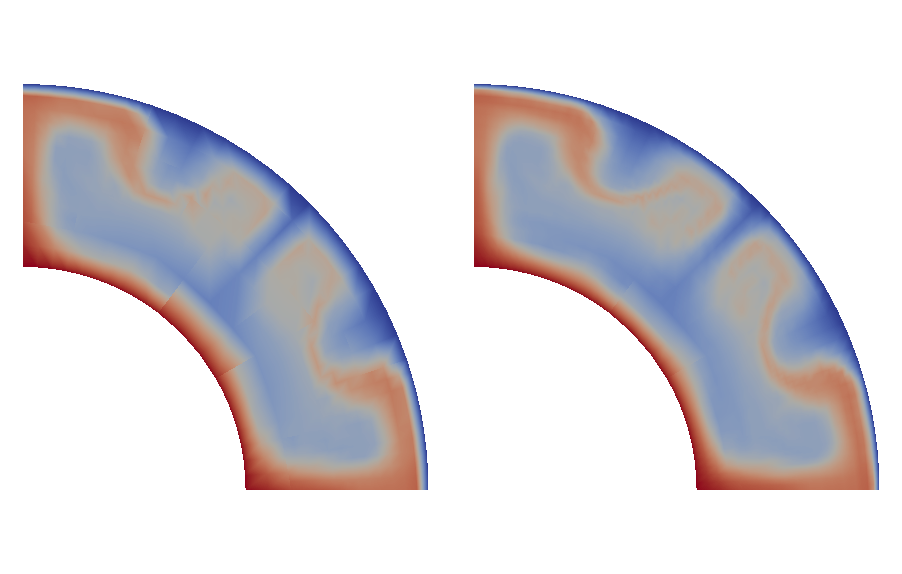
\includegraphics[width=0.5\textwidth]{viz/parameters/build-patches}\end{center}Here, the left picture shows one visualization cell per computational cell (i.e., the option is switch off, as is the default), and the right picture shows the same simulation with the option switched on. The images show the same data, demonstrating that interpolating the solution onto bilinear shape functions as is commonly done in visualizing data loses information.

Of course, activating this option also greatly increases the amount of data \aspect{} will write to disk: approximately by a factor of 4 in 2d, and a factor of 8 in 3d, when using quadratic elements for the velocity, and correspondingly more for even higher order elements.


{\it Possible values:} [Bool]
\item {\it Parameter name:} {\tt List of output variables}
\phantomsection\label{parameters:Postprocess/Visualization/List of output variables}


\index[prmindex]{List of output variables}
\index[prmindexfull]{Postprocess!Visualization!List of output variables}
{\it Value:} density, dynamic topography, strain rate, viscosity, shear stress, stress


{\it Default:} 


{\it Description:} A comma separated list of visualization objects that should be run whenever writing graphical output. By default, the graphical output files will always contain the primary variables velocity, pressure, and temperature. However, one frequently wants to also visualize derived quantities, such as the thermodynamic phase that corresponds to a given temperature-pressure value, or the corresponding seismic wave speeds. The visualization objects do exactly this: they compute such derived quantities and place them into the output file. The current parameter is the place where you decide which of these additional output variables you want to have in your output file.

The following postprocessors are available:

`Vp anomaly': A visualization output object that generates output showing the anomaly in the seismic compression wave speed $V_p$ as a spatially variable function with one value per cell. This anomaly is shown as a percentage change relative to the average value of $V_p$ at the depth of this cell.

`Vs anomaly': A visualization output object that generates output showing the anomaly in the seismic shear wave speed $V_s$ as a spatially variable function with one value per cell. This anomaly is shown as a percentage change relative to the average value of $V_s$ at the depth of this cell.

`artificial viscosity': A visualization output object that generates output showing the value of the artificial viscosity on each cell.

`density': A visualization output object that generates output for the density.

`dynamic topography': A visualization output object that generates output for the dynamic topography. The approach to determine the dynamic topography requires us to compute the stress tensor and evaluate the component of it in the direction in which gravity acts. In other words, we compute $\sigma_{rr}={\hat g}^T(2 \eta \varepsilon(\mathbf u)-\frac 13 (\textrm{div}\;\mathbf u)I)\hat g - p_d$ where $\hat g = \mathbf g/\|\mathbf g\|$ is the direction of the gravity vector $\mathbf g$ and $p_d=p-p_a$ is the dynamic pressure computed by subtracting the adiabatic pressure $p_a$ from the total pressure $p$ computed as part of the Stokes solve. From this, the dynamic topography is computed using the formula $h=\frac{\sigma_{rr}}{\|\mathbf g\| \rho}$ where $\rho$ is the density at the cell center.

Strictly speaking, the dynamic topography is of course a quantity that is only of interest at the surface. However, we compute it everywhere to make things fit into the framework within which we produce data for visualization. You probably only want to visualize whatever data this postprocessor generates at the surface of your domain and simply ignore the rest of the data generated.

`error indicator': A visualization output object that generates output showing the estimated error or other mesh refinement indicator as a spatially variable function with one value per cell.

`friction heating': A visualization output object that generates output for the amount of friction heating often referred to as $\tau:\epsilon$. More concisely, in the incompressible case, the quantity that is output is defined as $\eta \varepsilon(\mathbf u):\varepsilon(\mathbf u)$ where $\eta$ is itself a function of temperature, pressure and strain rate. In the compressible case, the quantity that's computed is $\eta [\varepsilon(\mathbf u)-\tfrac 13(\textrm{tr}\;\varepsilon(\mathbf u))\mathbf I]:[\varepsilon(\mathbf u)-\tfrac 13(\textrm{tr}\;\varepsilon(\mathbf u))\mathbf I]$.

`gravity': A visualization output object that outputs the gravity vector.

`internal heating': A visualization output object that generates output for the internal heating rate. Units: W/kg

`material properties': A visualization output object that generates output for the material properties given by the material model.There are a number of other visualization postprocessors that offer to write individual material properties. However, they all individually have to evaluate the material model. This is inefficient if one wants to output more than just one or two of the fields provided by the material model. The current postprocessor allows to output a (potentially large) subsets of all of the information provided by material models at once, with just a single material model evaluation per output point.

`melt fraction': A visualization output object that generates output for the melt fraction at the temperature and pressure of the current point (batch melting). Does not take into account latent heat. If there are no compositional fields, this postprocessor will visualize the melt fraction of peridotite (calculated using the anhydrous model of Katz, 2003). If there is at least one compositional field, the postprocessor assumes that the  first compositional field is the content of pyroxenite, and will visualize the melt fraction for a mixture of peridotite and pyroxenite (using the melting model of Sobolev, 2011 for pyroxenite). All the parameters that were used in these calculations can be changed in the input file, the most relevant maybe being the mass fraction of Cpx in peridotite in the Katz melting model (Mass fraction cpx), which right now has a default of 15\%. The corresponding p-T-diagrams can be generated by running the tests melt\_postprocessor\_peridotite and melt\_postprocessor\_pyroxenite.

`nonadiabatic pressure': A visualization output object that generates output for the non-adiabatic component of the pressure.

`nonadiabatic temperature': A visualization output object that generates output for the non-adiabatic component of the pressure.

`partition': A visualization output object that generates output for the parallel partition that every cell of the mesh is associated with.

`seismic vp': A visualization output object that generates output for the seismic P-wave speed.

`seismic vs': A visualization output object that generates output for the seismic S-wave speed.

`shear stress': A visualization output object that generates output for the 3 (in 2d) or 6 (in 3d) components of the shear stress tensor, i.e., for the components of the tensor $2\eta\varepsilon(\mathbf u)$ in the incompressible case and $2\eta\left[\varepsilon(\mathbf u)-\tfrac 13(\textrm{tr}\;\varepsilon(\mathbf u))\mathbf I\right]$ in the compressible case. The shear stress differs from the full stress tensor by the absence of the pressure.

`specific heat': A visualization output object that generates output for the specific heat $C_p$.

`strain rate': A visualization output object that generates output for the norm of the strain rate, i.e., for the quantity $\sqrt{\varepsilon(\mathbf u):\varepsilon(\mathbf u)}$ in the incompressible case and $\sqrt{[\varepsilon(\mathbf u)-\tfrac 13(\textrm{tr}\;\varepsilon(\mathbf u))\mathbf I]:[\varepsilon(\mathbf u)-\tfrac 13(\textrm{tr}\;\varepsilon(\mathbf u))\mathbf I]}$ in the compressible case.

`stress': A visualization output object that generates output for the 3 (in 2d) or 6 (in 3d) components of the stress tensor, i.e., for the components of the tensor $2\eta\varepsilon(\mathbf u)+pI$ in the incompressible case and $2\eta\left[\varepsilon(\mathbf u)-\tfrac 13(\textrm{tr}\;\varepsilon(\mathbf u))\mathbf I\right]+pI$ in the compressible case.

`thermal expansivity': A visualization output object that generates output for the thermal expansivity.

`thermodynamic phase': A visualization output object that generates output for the integer number of the phase that is thermodynamically stable at the temperature and pressure of the current point.

`viscosity': A visualization output object that generates output for the viscosity.

`viscosity ratio': A visualization output object that generates output for the ratio between dislocation viscosity and diffusion viscosity.


{\it Possible values:} [MultipleSelection Vp anomaly|Vs anomaly|artificial viscosity|density|dynamic topography|error indicator|friction heating|gravity|internal heating|material properties|melt fraction|nonadiabatic pressure|nonadiabatic temperature|partition|seismic vp|seismic vs|shear stress|specific heat|strain rate|stress|thermal expansivity|thermodynamic phase|viscosity|viscosity ratio ]
\item {\it Parameter name:} {\tt Number of grouped files}
\phantomsection\label{parameters:Postprocess/Visualization/Number of grouped files}


\index[prmindex]{Number of grouped files}
\index[prmindexfull]{Postprocess!Visualization!Number of grouped files}
{\it Value:} 0


{\it Default:} 0


{\it Description:} VTU file output supports grouping files from several CPUs into a given number of files using MPI I/O when writing on a parallel filesystem. Select 0 for no grouping. This will disable parallel file output and instead write one file per processor in a background thread. A value of 1 will generate one big file containing the whole solution, while a larger value will create that many files (at most as many as there are mpi ranks).


{\it Possible values:} [Integer range 0...2147483647 (inclusive)]
\item {\it Parameter name:} {\tt Output format}
\phantomsection\label{parameters:Postprocess/Visualization/Output format}


\index[prmindex]{Output format}
\index[prmindexfull]{Postprocess!Visualization!Output format}
{\it Value:} vtu


{\it Default:} vtu


{\it Description:} The file format to be used for graphical output.


{\it Possible values:} [Selection none|dx|ucd|gnuplot|povray|eps|gmv|tecplot|tecplot_binary|vtk|vtu|hdf5|svg|deal.II intermediate ]
\item {\it Parameter name:} {\tt Time between graphical output}
\phantomsection\label{parameters:Postprocess/Visualization/Time between graphical output}


\index[prmindex]{Time between graphical output}
\index[prmindexfull]{Postprocess!Visualization!Time between graphical output}
{\it Value:} 1.0


{\it Default:} 1e8


{\it Description:} The time interval between each generation of graphical output files. A value of zero indicates that output should be generated in each time step. Units: years if the 'Use years in output instead of seconds' parameter is set; seconds otherwise.


{\it Possible values:} [Double 0...1.79769e+308 (inclusive)]
\end{itemize}



\subsection{Parameters in section \tt Postprocess/Visualization/Dynamic Topography}
\label{parameters:Postprocess/Visualization/Dynamic_20Topography}

\begin{itemize}
\item {\it Parameter name:} {\tt Subtract mean of dynamic topography}
\phantomsection\label{parameters:Postprocess/Visualization/Dynamic Topography/Subtract mean of dynamic topography}


\index[prmindex]{Subtract mean of dynamic topography}
\index[prmindexfull]{Postprocess!Visualization!Dynamic Topography!Subtract mean of dynamic topography}
{\it Value:} false


{\it Default:} false


{\it Description:} Option to remove the mean dynamic topography in the outputted data file (not visualization). 'true' subtracts the mean, 'false' leaves the calculated dynamic topography as is. 


{\it Possible values:} [Bool]
\end{itemize}

\subsection{Parameters in section \tt Postprocess/Visualization/Material properties}
\label{parameters:Postprocess/Visualization/Material_20properties}

\begin{itemize}
\item {\it Parameter name:} {\tt List of material properties}
\phantomsection\label{parameters:Postprocess/Visualization/Material properties/List of material properties}


\index[prmindex]{List of material properties}
\index[prmindexfull]{Postprocess!Visualization!Material properties!List of material properties}
{\it Value:} density,thermal expansivity,specific heat,viscosity


{\it Default:} density,thermal expansivity,specific heat,viscosity


{\it Description:} A comma separated list of material properties that should be written whenever writing graphical output. By default, the material properties will always contain the density, thermal expansivity, specific heat and viscosity. The following material properties are available:

viscosity|density|thermal expansivity|specific heat|thermal conductivity|compressibility|entropy derivative temperature|entropy derivative pressure|reaction terms


{\it Possible values:} [MultipleSelection viscosity|density|thermal expansivity|specific heat|thermal conductivity|compressibility|entropy derivative temperature|entropy derivative pressure|reaction terms ]
\end{itemize}

\subsection{Parameters in section \tt Postprocess/Visualization/Melt fraction}
\label{parameters:Postprocess/Visualization/Melt_20fraction}

\begin{itemize}
\item {\it Parameter name:} {\tt A1}
\phantomsection\label{parameters:Postprocess/Visualization/Melt fraction/A1}


\index[prmindex]{A1}
\index[prmindexfull]{Postprocess!Visualization!Melt fraction!A1}
{\it Value:} 1085.7


{\it Default:} 1085.7


{\it Description:} Constant parameter in the quadratic function that approximates the solidus of peridotite. Units: $°C$.


{\it Possible values:} [Double -1.79769e+308...1.79769e+308 (inclusive)]
\item {\it Parameter name:} {\tt A2}
\phantomsection\label{parameters:Postprocess/Visualization/Melt fraction/A2}


\index[prmindex]{A2}
\index[prmindexfull]{Postprocess!Visualization!Melt fraction!A2}
{\it Value:} 1.329e-7


{\it Default:} 1.329e-7


{\it Description:} Prefactor of the linear pressure term in the quadratic function that approximates the solidus of peridotite. Units: $°C/Pa$.


{\it Possible values:} [Double -1.79769e+308...1.79769e+308 (inclusive)]
\item {\it Parameter name:} {\tt A3}
\phantomsection\label{parameters:Postprocess/Visualization/Melt fraction/A3}


\index[prmindex]{A3}
\index[prmindexfull]{Postprocess!Visualization!Melt fraction!A3}
{\it Value:} -5.1e-18


{\it Default:} -5.1e-18


{\it Description:} Prefactor of the quadratic pressure term in the quadratic function that approximates the solidus of peridotite. Units: $°C/(Pa^2)$.


{\it Possible values:} [Double -1.79769e+308...1.79769e+308 (inclusive)]
\item {\it Parameter name:} {\tt B1}
\phantomsection\label{parameters:Postprocess/Visualization/Melt fraction/B1}


\index[prmindex]{B1}
\index[prmindexfull]{Postprocess!Visualization!Melt fraction!B1}
{\it Value:} 1475.0


{\it Default:} 1475.0


{\it Description:} Constant parameter in the quadratic function that approximates the lherzolite liquidus used for calculating the fraction of peridotite-derived melt. Units: $°C$.


{\it Possible values:} [Double -1.79769e+308...1.79769e+308 (inclusive)]
\item {\it Parameter name:} {\tt B2}
\phantomsection\label{parameters:Postprocess/Visualization/Melt fraction/B2}


\index[prmindex]{B2}
\index[prmindexfull]{Postprocess!Visualization!Melt fraction!B2}
{\it Value:} 8.0e-8


{\it Default:} 8.0e-8


{\it Description:} Prefactor of the linear pressure term in the quadratic function that approximates the  lherzolite liquidus used for calculating the fraction of peridotite-derived melt. Units: $°C/Pa$.


{\it Possible values:} [Double -1.79769e+308...1.79769e+308 (inclusive)]
\item {\it Parameter name:} {\tt B3}
\phantomsection\label{parameters:Postprocess/Visualization/Melt fraction/B3}


\index[prmindex]{B3}
\index[prmindexfull]{Postprocess!Visualization!Melt fraction!B3}
{\it Value:} -3.2e-18


{\it Default:} -3.2e-18


{\it Description:} Prefactor of the quadratic pressure term in the quadratic function that approximates the  lherzolite liquidus used for calculating the fraction of peridotite-derived melt. Units: $°C/(Pa^2)$.


{\it Possible values:} [Double -1.79769e+308...1.79769e+308 (inclusive)]
\item {\it Parameter name:} {\tt C1}
\phantomsection\label{parameters:Postprocess/Visualization/Melt fraction/C1}


\index[prmindex]{C1}
\index[prmindexfull]{Postprocess!Visualization!Melt fraction!C1}
{\it Value:} 1780.0


{\it Default:} 1780.0


{\it Description:} Constant parameter in the quadratic function that approximates the liquidus of peridotite. Units: $°C$.


{\it Possible values:} [Double -1.79769e+308...1.79769e+308 (inclusive)]
\item {\it Parameter name:} {\tt C2}
\phantomsection\label{parameters:Postprocess/Visualization/Melt fraction/C2}


\index[prmindex]{C2}
\index[prmindexfull]{Postprocess!Visualization!Melt fraction!C2}
{\it Value:} 4.50e-8


{\it Default:} 4.50e-8


{\it Description:} Prefactor of the linear pressure term in the quadratic function that approximates the liquidus of peridotite. Units: $°C/Pa$.


{\it Possible values:} [Double -1.79769e+308...1.79769e+308 (inclusive)]
\item {\it Parameter name:} {\tt C3}
\phantomsection\label{parameters:Postprocess/Visualization/Melt fraction/C3}


\index[prmindex]{C3}
\index[prmindexfull]{Postprocess!Visualization!Melt fraction!C3}
{\it Value:} -2.0e-18


{\it Default:} -2.0e-18


{\it Description:} Prefactor of the quadratic pressure term in the quadratic function that approximates the liquidus of peridotite. Units: $°C/(Pa^2)$.


{\it Possible values:} [Double -1.79769e+308...1.79769e+308 (inclusive)]
\item {\it Parameter name:} {\tt D1}
\phantomsection\label{parameters:Postprocess/Visualization/Melt fraction/D1}


\index[prmindex]{D1}
\index[prmindexfull]{Postprocess!Visualization!Melt fraction!D1}
{\it Value:} 976.0


{\it Default:} 976.0


{\it Description:} Constant parameter in the quadratic function that approximates the solidus of pyroxenite. Units: $°C$.


{\it Possible values:} [Double -1.79769e+308...1.79769e+308 (inclusive)]
\item {\it Parameter name:} {\tt D2}
\phantomsection\label{parameters:Postprocess/Visualization/Melt fraction/D2}


\index[prmindex]{D2}
\index[prmindexfull]{Postprocess!Visualization!Melt fraction!D2}
{\it Value:} 1.329e-7


{\it Default:} 1.329e-7


{\it Description:} Prefactor of the linear pressure term in the quadratic function that approximates the solidus of pyroxenite. Note that this factor is different from the value given in Sobolev, 2011, because they use the potential temperature whereas we use the absolute temperature. Units: $°C/Pa$.


{\it Possible values:} [Double -1.79769e+308...1.79769e+308 (inclusive)]
\item {\it Parameter name:} {\tt D3}
\phantomsection\label{parameters:Postprocess/Visualization/Melt fraction/D3}


\index[prmindex]{D3}
\index[prmindexfull]{Postprocess!Visualization!Melt fraction!D3}
{\it Value:} -5.1e-18


{\it Default:} -5.1e-18


{\it Description:} Prefactor of the quadratic pressure term in the quadratic function that approximates the solidus of pyroxenite. Units: $°C/(Pa^2)$.


{\it Possible values:} [Double -1.79769e+308...1.79769e+308 (inclusive)]
\item {\it Parameter name:} {\tt E1}
\phantomsection\label{parameters:Postprocess/Visualization/Melt fraction/E1}


\index[prmindex]{E1}
\index[prmindexfull]{Postprocess!Visualization!Melt fraction!E1}
{\it Value:} 663.8


{\it Default:} 663.8


{\it Description:} Prefactor of the linear depletion term in the quadratic function that approximates the melt fraction of pyroxenite. Units: $°C/Pa$.


{\it Possible values:} [Double -1.79769e+308...1.79769e+308 (inclusive)]
\item {\it Parameter name:} {\tt E2}
\phantomsection\label{parameters:Postprocess/Visualization/Melt fraction/E2}


\index[prmindex]{E2}
\index[prmindexfull]{Postprocess!Visualization!Melt fraction!E2}
{\it Value:} -611.4


{\it Default:} -611.4


{\it Description:} Prefactor of the quadratic depletion term in the quadratic function that approximates the melt fraction of pyroxenite. Units: $°C/(Pa^2)$.


{\it Possible values:} [Double -1.79769e+308...1.79769e+308 (inclusive)]
\item {\it Parameter name:} {\tt Mass fraction cpx}
\phantomsection\label{parameters:Postprocess/Visualization/Melt fraction/Mass fraction cpx}


\index[prmindex]{Mass fraction cpx}
\index[prmindexfull]{Postprocess!Visualization!Melt fraction!Mass fraction cpx}
{\it Value:} 0.15


{\it Default:} 0.15


{\it Description:} Mass fraction of clinopyroxene in the peridotite to be molten. Units: non-dimensional.


{\it Possible values:} [Double -1.79769e+308...1.79769e+308 (inclusive)]
\item {\it Parameter name:} {\tt beta}
\phantomsection\label{parameters:Postprocess/Visualization/Melt fraction/beta}


\index[prmindex]{beta}
\index[prmindexfull]{Postprocess!Visualization!Melt fraction!beta}
{\it Value:} 1.5


{\it Default:} 1.5


{\it Description:} Exponent of the melting temperature in the melt fraction calculation. Units: non-dimensional.


{\it Possible values:} [Double -1.79769e+308...1.79769e+308 (inclusive)]
\item {\it Parameter name:} {\tt r1}
\phantomsection\label{parameters:Postprocess/Visualization/Melt fraction/r1}


\index[prmindex]{r1}
\index[prmindexfull]{Postprocess!Visualization!Melt fraction!r1}
{\it Value:} 0.5


{\it Default:} 0.5


{\it Description:} Constant in the linear function that approximates the clinopyroxene reaction coefficient. Units: non-dimensional.


{\it Possible values:} [Double -1.79769e+308...1.79769e+308 (inclusive)]
\item {\it Parameter name:} {\tt r2}
\phantomsection\label{parameters:Postprocess/Visualization/Melt fraction/r2}


\index[prmindex]{r2}
\index[prmindexfull]{Postprocess!Visualization!Melt fraction!r2}
{\it Value:} 8e-11


{\it Default:} 8e-11


{\it Description:} Prefactor of the linear pressure term in the linear function that approximates the clinopyroxene reaction coefficient. Units: $1/Pa$.


{\it Possible values:} [Double -1.79769e+308...1.79769e+308 (inclusive)]
\end{itemize}

\subsection{Parameters in section \tt Prescribed Stokes solution}
\label{parameters:Prescribed_20Stokes_20solution}

\begin{itemize}
\item {\it Parameter name:} {\tt Model name}
\phantomsection\label{parameters:Prescribed Stokes solution/Model name}


\index[prmindex]{Model name}
\index[prmindexfull]{Prescribed Stokes solution!Model name}
{\it Value:} 


{\it Default:} 


{\it Description:} Select one of the following models:

`circle': This value describes a vector field that rotates around the z-axis with constant angular velocity (i.e., with a velocity that increases with distance from the axis). The pressure is set to zero.


{\it Possible values:} [Selection circle ]
\end{itemize}

\subsection{Parameters in section \tt Termination criteria}
\label{parameters:Termination_20criteria}

\begin{itemize}
\item {\it Parameter name:} {\tt Checkpoint on termination}
\phantomsection\label{parameters:Termination criteria/Checkpoint on termination}


\index[prmindex]{Checkpoint on termination}
\index[prmindexfull]{Termination criteria!Checkpoint on termination}
{\it Value:} false


{\it Default:} false


{\it Description:} Whether to checkpoint the simulation right before termination.


{\it Possible values:} [Bool]
\item {\it Parameter name:} {\tt End step}
\phantomsection\label{parameters:Termination criteria/End step}


\index[prmindex]{End step}
\index[prmindexfull]{Termination criteria!End step}
{\it Value:} 100


{\it Default:} 100


{\it Description:} Terminate the simulation once the specified timestep has been reached.


{\it Possible values:} [Integer range 0...2147483647 (inclusive)]
\item {\it Parameter name:} {\tt Termination criteria}
\phantomsection\label{parameters:Termination criteria/Termination criteria}


\index[prmindex]{Termination criteria}
\index[prmindexfull]{Termination criteria!Termination criteria}
{\it Value:} end time


{\it Default:} end time


{\it Description:} A comma separated list of termination criteria that will determine when the simulation should end. Whether explicitly stated or not, the ``end time'' termination criterion will always be used.The following termination criteria are available:

`end step': Terminate the simulation once the specified timestep has been reached. 

`end time': Terminate the simulation once the end time specified in the input file has been reached. Unlike all other termination criteria, this criterion is \textit{always} active, whether it has been explicitly selected or not in the input file (this is done to preserve historical behavior of \aspect{}, but it also likely does not inconvenience anyone since it is what would be selected in most cases anyway).

`steady state velocity': A criterion that terminates the simulation when the RMS of the velocity field stays within a certain range for a specified period of time.

`user request': Terminate the simulation gracefully when a file with a specified name appears in the output directory. This allows the user to gracefully exit the simulation at any time by simply creating such a file using, for example, \texttt{touch output/terminate}. The file's location is chosen to be in the output directory, rather than in a generic location such as the Aspect directory, so that one can run multiple simulations at the same time (which presumably write to different output directories) and can selectively terminate a particular one.


{\it Possible values:} [MultipleSelection end step|end time|steady state velocity|user request ]
\end{itemize}



\subsection{Parameters in section \tt Termination criteria/Steady state velocity}
\label{parameters:Termination_20criteria/Steady_20state_20velocity}

\begin{itemize}
\item {\it Parameter name:} {\tt Maximum relative deviation}
\phantomsection\label{parameters:Termination criteria/Steady state velocity/Maximum relative deviation}


\index[prmindex]{Maximum relative deviation}
\index[prmindexfull]{Termination criteria!Steady state velocity!Maximum relative deviation}
{\it Value:} 0.05


{\it Default:} 0.05


{\it Description:} The maximum relative deviation of the RMS in recent simulation time for the system to be considered in steady state. If the actual deviation is smaller than this number, then the simulation will be terminated.


{\it Possible values:} [Double 0...1.79769e+308 (inclusive)]
\item {\it Parameter name:} {\tt Time in steady state}
\phantomsection\label{parameters:Termination criteria/Steady state velocity/Time in steady state}


\index[prmindex]{Time in steady state}
\index[prmindexfull]{Termination criteria!Steady state velocity!Time in steady state}
{\it Value:} 1e7


{\it Default:} 1e7


{\it Description:} The minimum length of simulation time that the system should be in steady state before termination.Units: years if the 'Use years in output instead of seconds' parameter is set; seconds otherwise.


{\it Possible values:} [Double 0...1.79769e+308 (inclusive)]
\end{itemize}

\subsection{Parameters in section \tt Termination criteria/User request}
\label{parameters:Termination_20criteria/User_20request}

\begin{itemize}
\item {\it Parameter name:} {\tt File name}
\phantomsection\label{parameters:Termination criteria/User request/File name}


\index[prmindex]{File name}
\index[prmindexfull]{Termination criteria!User request!File name}
{\it Value:} terminate-aspect


{\it Default:} terminate-aspect


{\it Description:} The name of a file that, if it exists in the output directory (whose name is also specified in the input file) will lead to termination of the simulation. The file's location is chosen to be in the output directory, rather than in a generic location such as the Aspect directory, so that one can run multiple simulations at the same time (which presumably write to different output directories) and can selectively terminate a particular one.


{\it Possible values:} [FileName (Type: input)]
\end{itemize}
